\documentclass{puthesis}

\usepackage{epsfig}
\usepackage{amsfonts}
\usepackage{amssymb}
\usepackage{amsmath}   
\usepackage{amsthm}
\usepackage{latexsym}

\usepackage{nohyperref}
\usepackage{url}
\usepackage{bm}
\usepackage{xparse}
\usepackage{placeins}
\usepackage{float}
\usepackage{booktabs}
\usepackage{longtable}
\usepackage{colortbl}
\usepackage{epigraph}

\renewcommand{\epigraphsize}{\small}

\setlength{\epigraphwidth}{0.8\textwidth}

\renewcommand{\textflush}{flushright} \renewcommand{\sourceflush}{flushright}

\let\originalepigraph\epigraph 
\renewcommand\epigraph[2]{\originalepigraph{#1}{\textsc{#2}}}

% set font
\usepackage[T1]{fontenc}
\usepackage[utf8]{inputenc}
\usepackage{pifont}
\usepackage{newunicodechar}
\newunicodechar{✓}{\ding{51}}
\newunicodechar{✗}{\ding{55}}

% argmax/argmin
\DeclareMathOperator*{\argmax}{arg\,max}
\DeclareMathOperator*{\argmin}{arg\,min}

% add ubar command
\usepackage{accents}
\DeclareRobustCommand{\ubar}[1]{\underaccent{\bar}{#1}}

% Expectation, Variance, Covariance
\newcommand{\E}{\mathrm{E}}
\newcommand{\Var}{\mathrm{Var}}
\newcommand{\Cov}{\mathrm{Cov}}

% https://github.com/rstudio/rmarkdown/issues/1649
\newlength{\cslhangindent}
\setlength{\cslhangindent}{1.5em}
\newenvironment{cslreferences}%
  {\setlength{\parindent}{0pt}%
  \everypar{\setlength{\hangindent}{\cslhangindent}}\ignorespaces}%
  {\par}

\NewDocumentCommand{\evalat}{sO{\big}mm}{%
  \IfBooleanTF{#1}
   {\mleft. #3 \mright|_{#4}}
   {#3#2|_{#4}}%
}

\makeatletter\def\Hy@xspace@end{}\makeatother

\title{Trade Policy in the Shadow of Power\\
\tiny \hfill\\
\Large Theory and Evidence on Economic Openness and Coercive Diplomacy}
\submitted{November 2020}  %graduation date
\author{Brendan Michael Cooley}
\abstract{This dissertation studies military coercion in the
international political economy. I develop a framework to study how
power politics affects the international economy and how conflicts of
interest over economic policy affect states' propensity to fight wars
with one another. I begin by building a theoretical model of ``gunboat
diplomacy,'' in which wars can be fought in order to open markets
abroad. The shadow of military power liberalizes trade policy, and more
protectionist governments are more likely to experience war. I then
introduce an empirical model to measure the magnitude of policy-induced
trade frictions, which I estimate on data describing trade flows, price
levels, and freight costs in 2011. Finally, I rationalize the emergence
of these barriers as the outcome of an \(N\)-country coercive bargaining
game, in order to quantify empirically the effect of military coercion
on international trade. In the aggregate, military coercion increases
the value of global trade by 63 percent, suggesting that international
power politics exerts substantial influence on the workings of the
international economy.}
\adviser{Kristopher W. Ramsay}
\acknowledgements{I learned I wanted to become a political scientist as
a junior at the University of North Carolina at Chapel Hill. Stephen
Gent and Navin Bapat quickly taught me enough about the discipline to
enable me convince one graduate admissions committee that I deserved a
shot at a Ph.D.~

\par

When I arrived at Princeton, Saurabh Pant and Ted Enamorado introduced
me to mathematical analysis and were models of competence and
professionalism as graduate student instructors. Every course I took at
Princeton -- in Politics, Economics, or Operations Research -- sparked
new ideas or equipped me with tools I needed to do my research. The set
of things that I knew I did not know continually expanded throughout my
time in graduate school, even as I took courses well into my fourth year
of graduate school in futile hope of reducing the number of these
things.

\par

The Politics Department maintained a culture that encouraged
intellectual curiosity and collegiality. Corwin 127 was never a
particularly functional classroom or seminar room yet I will remember it
fondly as the embodiment of this culture. Richard Jordan, Ryan Brutger,
and Austin Wright gave practice job talks there in my first year that
served as exemplars for what I hoped to achieve in a dissertation for
the rest of my time in graduate school.

\par

In addition to engaging courses and a supportive culture, Princeton
University provided substantial material support that faciliated the
completion of this dissertation. The Fellowship of Woodrow Wilson
Scholars relieved me of the responsibility to teach in my fourth and
fifth years. The Program in Quantitative and Analytical Political
Science and the Niehaus Center provided me with office space. The
Research Program in Political Economy helped me purchase data. I did not
anticipate needing to purchase Australian customs records when I started
graduate school. The papers embedded in this dissertation also benefited
from the feedback of audiences at many conferences: the American
Political Science Association's annual meeting (2019, 2020), the Midwest
Political Science Association's annual meeting (2018, 2019), the
Southern Political Science Association's annual meeting (2019, 2020) the
International Studies Association's annual meeting (2019) and Midwest
meeting (2019), the Online Peace Science Colloquium (2019), and the
Formal Models of International Relations conference at Vanderbilt
(2020).

\par

Learning how to do research often involved chaotic spurts of searching
the internet for solutions to some thankless data analysis problem. This
turned out to be a remarkably effective problem solving method, thanks
to the public goods provision of a small army of programmers and
researchers active on Github and Stack Exchange. I could not have
completed this dissertation without the enormous ecosystem of open
source software developed by this army and others. I have done my best
to cite the software packages I used to produce this dissertation at the
end of the manuscript. These are the but the tip of an incredibly useful
iceberg.

\par

I pitched the skeleton of the idea that would turn into this
dissertation to Kris Ramsay at the beginning of my second year. Kris,
who would become my adviser, encouraged me to take a course
international trade in the Economics Department despite my reservations.
I was extraordinarily fortunate to receive this guidance in retrospect.
I quickly learned that trade was a far richer subfield than my training
in political science had led me to believe, and trade models became the
engines underneath my entire dissertation project. Matias Iaryczower
taught me a new way to think about empirical social science. Helen
Milner retained a healthy skepticism toward my ideas, pushed me to
defend my assumptions, and continually referred me to others' research
that made my work better. Melissa Lee did not serve on my dissertation
committee but was nevertheless a constant sorce of encouragement and
welcome diversionary chats about baseball.

\par

My research ended up being somewhat strange by the standards of the
discipline and sometimes struggled to find an academic community to call
home. Several faculty members outside of Princeton went out of their way
to support me nevertheless. Rob Carroll, Brenton Kenkel, Mike Gibilisco,
Brad Smith, and Scott Abramson took interest in my work and served as
helpful sounding boards for my ideas.

\par

I was blessed to matriculate at Princeton with a cohort full of good
people. Noam Reich, Mike Kistner, Elsa Voytas, Dan Gibbs, and Will Horne
in particular made life outside of writing, coding, and coursework
enjoyable. Poker games, barbequeues, and late night trips to the batting
cages were always welcome distractions from work. Korhan Koçak and
Naijia Liu made me happy to show up to the office every morning.

\par

Despite all of this support, completing a dissertation remains a largely
solitary endeavor. My friends and family outside of Princeton helped
make it feel less so. The highlight of every year I spent in graduate
school was a summer trip into the woods of California, Colorado, or
upstate New York with Shawn, Joe, and Andy. Someday we will manage to
implement all of the exceptional business ideas hatched on those trips.
Central New Jersey was an ideal launch pad to visit my family, most of
whom were dispersed between Boston and Washington, DC. My brothers
remain my best friends. My parents, trained in science and engineering,
were nothing but supportive of my decision to study a ``soft'' science.

\par

I met Sarah for dinner on the Delaware River in New Hope, PA in on a
cold February night in my second year and she quickly became the most
important person in my life. I got turned around in the parking lot that
night but have been headed in the right direction ever since.}

\begin{document}

\addcontentsline{toc}{chapter}{Introduction}

\chapter*{Introduction}

\epigraph{The relationship between economics and politics...is a reciprocal one. On the one hand, politics largely determines the framework of economic activity and chanels it in directions intended to serve the interests of dominant groups; the exercise of power in all its forms is a major determinant of the nature of an economic system. On the other hand, the economic process itself tends to redistribute power and wealth; it transforms the power relationships among groups.}{Robert Gilpin, \textit{U.S. Power and the Multinational Corporation}}

Why does war recur? The field of international relations has remained
preoccupied with this question since its genesis. This preoccupation is
well-justified. Warfare's costs -- measured in lives lost, property
destroyed, and productive resources reallocated -- are immense (Lacina
and Gleditsch 2005; Coe 2011). Wars also reshape the international
political order, redistributing political power and economic resources
among states and affecting the material welfare of belligerents and
non-belligerents alike (Gilpin 1981). The Second World War, for example,
not only revealed mankind's destructive potential but also shaped the
world that came after it, dividing it into distinct political orders and
circumscribing the opportunities available to those living within each
for decades thereafter (Ikenberry 2011).

Contemporary international relations theory conceptualizes war as an
outcome of a bargaining process between governments (Schelling 1960;
Fearon 1995). Wars recur because of \emph{bargaining frictions},
information asymmetries or time consistency problems, that prevent the
governments from finding a peaceful resolution to the conflict at hand.
Diagnosing the cause of a given war requires identifying the bargaining
friction that prevented the belligerents from settling their dispute
peacefully (Lake 2010). Systematic variation in the intensity of these
bargaining frictions explains variation in governments' propensity to
experience war (Lemke and Werner 1996; Schultz 1999; Reed 2003; Reed et
al. 2008).

The bargaining model is agnostic on the ends governments seek in
international bargaining interactions. The existence of some conflict of
interest, a disagreement about optimal joint behavior, is assumed by the
model. Territory, or some other rival good, is often assumed to be the
object of contention between governments. Yet states often forgo the
opportunity to seize territory, even when doing so is costless (Schultz
and Goemans 2019). This ``territorial peace'' (Gibler and Tir 2014) has
not obviated international conflicts of interest. Diplomats remain
engaged with one another on issues of trade, investment, monetary
policy, and migration due to the externalities that governments' actions
in these issue areas impose on other governments. Contemporary
U.S.-China relations are plagued by hostility and the spectre of war
between the two countries structures defense planning on both sides of
the Pacific Ocean. However, neither Beijing nor Washington makes claims
on the other's territory. Despite this territorial peace, conflicts over
commercial policy, manifesting in a trade war in 2018, complicate
Sino-U.S. diplomatic rapprochement.\footnote{Taplin, Nathaniel. ``Meet
  the New Trade War. It's Not the Same as the Old Trade War.'' \emph{The
  Wall Street Journal}. 7 May 2020.}

Negotiations over such economic issues are often relegated practically
and analytically to the realm of ``low politics.'' Ministries of foreign
affairs maintain separate offices for the ``high'' political issues of
territorial integrity and national security and the ``low'' political
issues of international economics. The scholarly field of international
relations enforces a division of labor between Security Studies and
International Political Economy (IPE). These divisions suggest that high
and low politics are largely separable -- negotiations over trade,
investment, monetary, and migration policy depend little on arms and
military alliances.

The primary purpose of this dissertation is to demonstrate theoretically
and empirically that the analytical distinction between high and low
politics is unproductive. I provide a framework to study how
international power politics affects the international economy and how
conflicts of interest over economic policy affect states' propensity to
fight wars with one another. High and low politics are inextricably
intertwined.

I focus my attention on trade policy conflicts of interest in
particular. There are practical and substantive reasons for doing so.
Practically, dramatic advances in empirical trade economics have enabled
researchers to study the effects of counterfactual trade policy regimes.
I use these tools to measure the magnitude of aggregate trade policy
distortions and rationalize their emergence as the outcome of a coercive
bargaining process between governments. Substantively, patterns of
international economic exchange dramatically affect human welfare.
Aforementioned empirical trade models suggest that, for the average
country, international exchange increases consumer welfare between 4 and
40 percent, relative to global autarky (Costinot and Rodríguez-Clare
2015). Perhaps more importantly, trade policy dramatically affects the
distribution of welfare across individuals and firms within the same
country (Autor, Dorn, and Hanson 2013; Fajgelbaum and Khandelwal 2016;
Waugh 2019; Caliendo, Dvorkin, and Parro 2019). As a result, commercial
policy at home and abroad attracts the attention of special interest
groups, which seek to influence governments' policy choices (Mayer 1984;
Rogowski 1987; Grossman and Helpman 1994; Osgood 2016; Kim 2017; Gulotty
2020). For firms and individuals alike, trade policy can be an
existential question. Burgess and Donaldson (2010) document a
relationship between trade costs and the prevalence of famine. For
firms, tariff liberalizations affect the probability of market exit
(Baggs 2005). The stakes of trade policy are high.

The ``Wisconsin School'' of diplomatic history places the domestic and
international distributional effects of trade policy at the center of an
account of U.S. foreign policy from the late 19th century through the
Cold War (Williams 1959; LaFeber 1963; McCormick 1967; Fordham 1998,
2019). American foreign policy -- the arms it procured and the wars it
prosecuted -- was designed largely to ensure U.S. trade policy autonomy
against foreign influence or open markets abroad. Those influencing and
crafting U.S. foreign policy did so at the behest of economic interests
that stood to benefit from protectionist tariffs or reductions in
barriers to enter foreign markets. Foreign policy served the ends of a
broader commercial policy. Different combinations of organized interests
enjoy access to governments outside the United States, but trade policy
shapes their welfare in much the same way. Lake (2014) argues that the
trade policy orientations of dominant interest groups in the United
States and China will determine the tenor of Sino-U.S. relations in the
21st century.

Channeled through political institutions, economic interests affect
foreign policy (Lake 2009). Governments' joint foreign policies in turn
shape the international economy. The victors of World War II exploited
their military position to impose rival sets of economic institutions,
rules governing international trade, on other governments within their
political orbits (McKenzie 2008). These economic institutions shaped the
flow of world trade throughout the Cold War and the development
prospects of the economies embedded within each regime (Gowa and
Mansfield 1993).

The dissertation's first chapter connects low politics to high politics
theoretically. I build a model of ``gunboat diplomacy'' in which wars
can be fought in order to open markets abroad. Political economic
incentives affect governments' incentives to fight wars -- governments
that place greater weight on firm profits relative to consumer welfare
are more belligerent in their foreign policy orientation. Even when
peace prevails, the shadow of military power affects trade policy.
Militarily powerful governments need not succumb to foreign threats,
resulting in more protectionist trade policies. The high politics of
coercive diplomacy affects trade policy. The low politics of market
access affects governments' incentives to prosecute wars.

Connecting high and low politics empirically requires first
operationalizing the explicandum -- trade policy. Tariffs levels are
widely used as a measure of protectionism, but tariffs are but one
method through which governments distort the flow of trade. In the
dissertation's second chapter, I produce estimates of the magnitude of
aggregate policy-induced trade distortions between pairs of countries.
This measurement exercise involves developing a model of the
international economy that connects latent trade policy distortions to
cross-national price levels, trade flows, and freight costs between
pairs of countries. With data on the latter quantities, the model can be
used to quantify the magnitude of latent trade policy frictions. I find
that policy barriers to trade are an order of magnitude larger than
tariffs in ad valorem terms on average, and that market access
conditions vary dramatically across the sample of countries studied. A
subset of developed countries enjoy far lower barriers to their exports
than do their developing peers.

I proceed to measure empirically the exercise of military power in
international relations and quantify its effects on the international
economy in the dissertation's final chapter. To borrow the definition of
Dahl (1957), a government has power over another to the extent that it
can get that government to do something it otherwise would not do.
Attributing trade policy to the exercise of power requires knowledge of
this counterfactual -- what policy would the government enact in power's
absence? Liberal trade policies might reflect domestic political
economic incentives for openness. Alternatively, they may reflect the
military constraints of the anarchic international system. To
disentangle these competing explanations, I model observed trade
policies as the outcome of an \(N\)-country coercive bargaining game.
Trade policy favoritism -- which countries are granted preferential
market access -- identify parameters governing the costs of war. I find
that military power confers bargaining advantage by reducing the costs
of war, promoting trade liberalization. In the aggregate, military
coercion increases the value of global trade by 63 percent.

Calculating this change in the value of global trade requires conducting
a counterfactual experiment, asking the model what would happen if
coercion was impossible. Once estimated, the model allows me to answer
this question and many others that empirically connect high and low
politics. How would changing governments' underlying preferences for
protectionism affect the probability of war? How would changing the
distribution of military power in the international system affect trade
policy and the international economy?

Answering these questions using quasi-experimental methods would be
extremely challenging. Random variation in governments' preferences or
military capabilities is difficult to come by. Even where such variation
exists, the local effects of this variation may not generalize globally.
My approach to these questions relies on theory to fill in gaps in the
data. Taking this approach means that the answers I give to these
questions take on a conditional form. If the assumptions embedded in the
model obtain, then changes to model primitives (power or preferences)
can be connected to changes in model output (trade policy and trade
flows). This ``structural'' econometric approach has the virtue of
transparency. Other researchers can examine the predictions made by my
model, evaluate their fidelity to the data, and compare them to the
predictions of alternative models. This process may highlight new
empirical puzzles and shortcomings of existing theories, furthering the
collective scholarly process of aligning theory and data.

War remains a rare event in contemporary international politics.
However, as relations between the world's largest economies (China and
the United States) demonstrate, antagonistic and militarized
international relations persist. While governments actively design
institutions to manage these conflicts short of war, our existing
understanding of international conflict highlights how fragile such
arrangements are -- small changes to governments' information sets or
their expected future strengths can trigger war. Achieving ``perpetual
peace'' requires not only eliminating warfare, but the abolition of
standing armies and international agreements that entertain the
possibility of future conflict. In other words, achieving the Kantian
ideal requires the elimination of conflicts of interest. Clearly, the
peace we enjoy in the 21st century remains far from this Kantian ideal.
This dissertation studies the conflicts of interest that undergird
international antagonisms, in hopes of progress toward understanding the
conditions that encourage their termination.

\chapter[Gunboat Diplomacy: Political Bias, Trade Policy, and War]{Gunboat Diplomacy \\ \Large Political Bias, Trade Policy, and War}

\section{Introduction}

Countries with deep trading relationships rarely fight wars with one
another. Some argue this ``commercial peace'' is due to the pacifying
effect of trade --- trade causes peace.\footnote{This literature is
  vast. See Gartzke and Zhang (2015) for a complete survey. Angell
  (1911), Polachek (1980), and Philippe, Mayer, and Thoenig (2008) are
  representative of this view.} Others say amicable political relations
cause trade.\footnote{See, for example, Pollins (1989b), Barbieri and
  Levy (1999), Benson and Niou (2007)} Trade is usually considered to be
exogenous to conflicts of interest in international relations.
Governments are posited to fight wars over territorial, ideological, or
other non-economic conflicts of interest. Preexisting trade relations
make these conflicts more costly, and less likely as a result.

Yet, trade policy is itself a central object of contention in
international relations. Governments are mercantilist to some extent
(Gawande, Krishna, and Olarreaga 2009). They desire some degree of
protection at home and ``open doors'' abroad and have historically been
willing to fight wars to compel market openness abroad.\footnote{See
  Findlay and O'Rourke (2007) for a chronicle of trade conflicts over
  the past millennium.} In the 1850s, the U.S. gunboats compelled an
autarkic Japanese government to open its markets. Britain and France
prosecuted the Opium Wars (1839-1842; 1856-1860) to compel a
recalcitrant Chinese government to reform its trade policies. Recently,
a proposal to integrate the economies of Ukraine and the European Union
led to war between Ukraine and Russia.\footnote{In this case, Moscow
  conditioned its coercion on the trade policy choices of Kiev, see
  James Marson and Naftali Bendavid,
  \href{https://www.wsj.com/articles/poroshenko-says-eu-agreement-to-be-ratified-next-week-1410519009}{``Ukraine
  to Delay Part of EU Pact Opposed by Russia,''} \emph{The Wall Street
  Journal}, 12 September 2014.} These episodes highlight linkages
between trade policy and war. But such linkages may be more common, as
the absence of war need not imply the absence of coercive bargaining
(Fearon 1995).

Here, I develop a theory of trade policy bargaining in the shadow of
military power, or ``gunboat diplomacy.'' The value of international
trade flows and the probability of peace are positively correlated in
equilibrium. This correlation emerges not because trade causes peace.
Rather, liberal trade policy preferences generate incentives for both
trade and peace. When peace prevails, latent military threats influence
equilibrium trade policies, which balance domestic political-economic
interests against military threats from abroad. Militarily weak
countries are more open to trade than powerful ones, all else equal.

The model considers the interaction between two governments (home and
foreign), which each value a weighted average of consumer welfare and
firm profits. These components of government utility themselves depend
on the workings of an underlying ``new trade'' international economy
(Krugman 1980; Venables 1987). Governments differ in how much influence
consumers have over policymaking.\footnote{This setup mirrors Grossman
  and Helpman (1994).} I refer to this variation as the governments'
degree of political \emph{bias}.\footnote{This phraseology borrows from
  Jackson and Morelli (2007). In their model, political bias determines
  the extent to which the pivotal decision maker internalizes the costs
  of war. Conceptually, bias is similar to the size of the selectorate
  in the model of Bueno De Mesquita et al. (2003).} Tariffs help firms
by shielding them from competition, but raise prices for consumers.
\emph{Low bias} or \emph{liberal} governments prefer lower tariffs.

Governments care about trade policy choices abroad because of market
access externalities (Ossa 2011, 2012). Firms' profits depend on their
ability to access foreign markets. High tariffs shift profits from
foreign to home firms. Therefore, firms on opposite sides of a border
experience a conflict of interest over trade policy. Firms desire
protection at home and liberalization abroad. The greater their bias,
the more the governments internalize these interests.

As a consequence, governments themselves experience conflicts of
interest over trade policy, which vary as a function of the governments'
bias. When governments value consumer welfare, they prefer to adopt low
barriers to trade. In doing so, they impose small market access
externalities on their trading partners. When both governments hold
liberal policy preferences, their relations are harmonious -- there is
no incentive for conflict, militarized or otherwise. As governments
become less liberal, conflicts of interest become more severe.

If a government wins a war, it earns the right to impose regime change
and install a ``puppet'' government abroad.\footnote{See Owen IV (2002)
  for an empirical study of regime change.} Puppets open their markets
to foreign firms, allowing victorious governments to impose their trade
policy preferences by force. This is the threat point governments
leverage in bilateral trade policy negotiations. War sometimes occurs
due to information frictions.

Two primary insights emerge from this environment. First, governments'
degree of bias affects their propensity to trade and fight wars. When
both governments are liberal, the costs of regime change never exceed
its policy benefits. As a result, highly liberal governments never fight
wars with one another. Their liberal preferences also result in liberal
equilibrium trade policies. Naturally, lowering barriers to trade
increases trade itself. The governments' preference compatibility
produces a relationship between trade and peace, but this relationship
is spurious --- trade itself has no pacifying effect. Second, even when
governments avoid conflict, trade policies reflect the balance of
military power between the governments. Powerful countries can credibly
threaten to impose regime change. They leverage this power to extract
trade policy concessions and resist liberalization. After bargaining,
powerful countries are more protectionist than weaker ones.

The model rationalizes several well-established empirical facts in
international relations. Bilateral trade tends to decrease before wars
and rebound thereafter.\footnote{This relationship is shown in Figure
  \ref{fig:tradeRD} in the Appendix.} In the model, protectionist
preference shocks decrease trade, but also increase the likelihood of
war. As a consequence, periods of depressed trade correlate with war
onset. Conversely, regime change following war causes a liberal
preference shock to the losing country's government. Trade increases
after wars, as in the data.

Some argue democracies have more liberal trade policy preferences than
autocracies (Milner and Kubota 2005). Because consumers (voters) prefer
free trade, they punish protectionist politicians (Mayer 1984; Grossman
and Helpman 1996).\footnote{For a skeptical take on this mechanism, see
  Guisinger (2009) and Betz and Pond (2019).} This provides a check on
the protectionist influence of special interest groups. Translated into
this framework, these theories deem democracies less biased than
autocracies. If this ``liberal democracy'' hypothesis holds, the
analysis of low bias governments extends to democratic dyads. The model
then jointly rationalizes the democratic peace and democracies'
propensity for trade openness.\footnote{These facts are depicted in
  Figure \ref{fig:comdempeace} in the Appendix. For a recent review on
  the relationship between democracy and peace, see Reiter (2017).
  Milner and Kubota (2005) show democratization tends to lead to
  decreased protectionism.}

The theory's implications about power and protectionism are, as far as I
know, novel. I consider these empirical implications in more detail in
the Discussion section. There, I also relate the theory to militarism,
imperialism, and territorial conflict.

Antràs and Padró i Miquel (2011) and Carroll (2018) are two closely
related papers that merit some discussion. Antràs and Padró i Miquel
(2011) consider a similar model, in which foreign governments can
interfere in the domestic political economy of trade. As in this model,
foreign influence has a liberalizing effect. In the anarchy of world
politics, however such influence can always -\/-- in principle -\/--
take the form of threats, displays, or uses of military force (Fearon
1997). Analyzing this form of influence allows me to relate the domestic
political economy of trade to military power and conflict propensity.
Carroll (2018) unifies militarized competition and economic exchange in
a more general setting. There, countries' convert commodities into
military power, which can in turn be employed to seize others'
commodities. Military power itself is endogenous to the general
equilibrium of the international economy. I take power as exogenous and
focus on competition over trade \emph{policy}. This more narrow focus
allows me to incorporate domestic political economy considerations and
make empirical predictions about power, trade policy, and war.

Others have considered policy competition in the shadow of power more
generally. Bils and Spaniel (2017) study a model of coercive bargaining
over the location of a spatial policy. Like the model studied here,
governments vary in the location of their ideal points. They study how
uncertainty over the states' ideal points affects conflict propensity.
Here, I microfound governments' preferences with a political economy of
trade policy and explore how domestic political economic shocks affect
the international bargaining environment. This generates unique
comparative statics and empirical implications.

\section{Environment}

Here and in the Analysis section, I relegate proofs and derivations of
key quantities to the Appendix, in order to ease exposition. I first
present the context in which governments bargain, followed by the
international economy. The general equilibrium of the economy determines
how trade policies affect prices, wages, and trade flows. These in turn
determine the welfare of consumers, firms, and the governments that
represent them. Proposition \texttt{1}, presented in this section,
states that given our assumptions, an \emph{economic equilibrium}
(Definition \texttt{2}) will exist for any feasible trade policy
choices. This economy allows us to write government preferences as an
indirect function of trade policy choices. As governments become more
liberal, they prefer to adopt low barriers to trade. This variation
affects how governments behave in the coercive bargaining game that
follows.

\subsection{International Bargaining}

Two governments, home (\(i\)) and foreign (\(j\)) bargain over their
joint trade policies
\(\bm{\tau} = \left( \tau_i, \tau_j \right) \in [1, \bar{\tau}]^2\).\footnote{Here,
  \(\bar{\tau}\) is an arbitrary prohibitively high tariff that shuts
  down bilateral trade.} By controlling the degree of market access
afforded to foreign firms, governments' trade policies impose
externalities on one another. Government preferences depend on an
exogenous parameter \(a_i \in [\ubar{a}, \bar{a}]\), which controls the
value these governments place on consumer welfare, relative to firm
profits.\footnote{\(\bar{a}\) is defined below.} Government utility is
denoted \(G_i( \bm{\tau} | a_i)\).\footnote{I develop the international
  economy from the home country's perspective, but analogous primitives
  exist for the foreign country.} Higher tariffs increase firm profits
by shifting market share to local firms. This comes at the expense of
consumers, however, who benefit from having access to a variety of
products, home and foreign. Higher tariffs also harm foreign firms and
the foreign government. This is the model's core conflict of interest.
Each government would like to implement some degree of protectionism at
home, while maintaining access to markets abroad.

Bargaining occurs in the shadow of power. Government \(i\) makes a
take-it-or-leave-it (TIOLI) offer
\(\tilde{\bm{\tau}} = \left( \tilde{\tau}_i, \tilde{\tau}_j \right)\) to
Government \(j\). Government \(j\) can either accept the offer or
declare war, a choice denoted with
\(\omega \in \left\{ \text{accept}, \text{war} \right\}\). This is a
simple coercive bargaining framework following Fearon (1995).\footnote{While
  this bargaining protocol is restrictive, Fey and Kenkel (2019) show
  more complex bargaining processes are equivalent to a TIOLI offer in
  terms of their associated payoffs and probability of war.} Here,
however, war results in \emph{regime change}, rather than a simple
costly division of a fixed surplus. Regime change is modeled as a change
in a vanquished government's \emph{preferences}. If government \(i\)
wins a war, it replaces the government of its counterpart, fixing its
preference parameter at \(a^\star\). \(\rho\) denotes the probability
that Government \(i\) is successful in a war for regime
change.\footnote{With complementary probability, the initiating
  government is overthrown. A more realistic formulation might allow for
  the possibility that no regime change occurs, with
  \(\rho_i + \rho_j \leq 1\). While this ``all or nothing'' conception
  of war is stark, it simplifies the analysis and highlights the forces
  at play.} \(c_i\) is the cost that government \(i\) must pay if a war
occurs. \(c_j > 0\) is held as private information. Government \(i\)
believes \(c_j\) is distributed according to \(F\) where \(F\) is the
uniform c.d.f. on \([\ubar{c}_j, \bar{c}_j]\).

As is standard in bargaining models of war, the costs of war must be
bounded, or the proposing country will never risk conflict. Assumption
\texttt{1} formalizes this intuition.

\textbf{Assumption 1:} \(\bar{c}_j \leq \kappa_j\) and
\(c_i < \kappa_i(\bar{c}_j)\) where \(\kappa_j\) and
\(\kappa_i(\bar{c}_j)\) are positive constants defined in the Appendix.

A strategy for Government \(i\) is an offer,
\(\tilde{\bm{\tau}}(a_i, c_i, \rho)\). A strategy for Government \(j\),
denoted \(\omega(\tilde{\bm{\tau}}; a_j, c_j, \rho)\) is a mapping
between this offer and a choice of whether or not to attempt regime
change \[
\omega : \tilde{\bm{\tau}} \rightarrow \left\{ \text{accept}, \text{war} \right\} .
\] Let \(\tilde{G}_k(\tilde{\bm{\tau}}, \omega | a_k, c_k, \rho)\)
denote government \(k\)'s utility as a function of these choices. From
these objects we can define a subgame perfect bargaining equilibrium.

\textbf{Definition 1:} A subgame perfect \emph{bargaining equilibrium}
is pair of strategies, \(\tilde{\bm{\tau}}^\star(a_i, c_i)\) and
\(\omega^\star(\tilde{\bm{\tau}}; a_j, c_j)\) such that \[
\omega^\star(\tilde{\bm{\tau}}; a_j, c_j, \rho) = \argmax_{\omega \in \left\{\text{accept}, \text{war} \right\}} \tilde{G}_j \left(\tilde{\bm{\tau}}, \omega; a_j, c_j, \rho \right)
\] and \[
\tilde{\bm{\tau}}^\star(a_i, c_i, \rho) \in \argmax_{\bm{\tau} \in [1, \bar{\tau}]^2} \mathbb{E}_{f(c_j)} \left[ \tilde{G}_i \left(\tilde{\bm{\tau}}, \omega^\star(\tilde{\bm{\tau}}; a_j, c_j, \rho); a_i, c_i, \rho \right) \right] .
\]

\subsection{International Economy}

Government preferences in the game described above depend on the
mechanics of the international economy. To simplify the presentation and
focus on the dynamics of coercive bargaining in this political economy,
I consider the special case in which countries are mirror images of one
another in terms of their economic primitives. Each country is inhabited
by a representative consumer with labor endowment \(L_i = L_j = L\).
Consumers value varieties of manufactured goods and goods from an
undifferentiated outside sector, which I'll call agriculture. By
providing their labor to local producers of these goods, they earn an
endogenous wage \(w_i\). Consumers' income inclusive of tariff revenues
\(r_i(\tau_i)\) is \(I_i(\tau_i) = w_i L_i + r_i(\tau_i)\). A unit of
labor can produce one unit of both differentiated goods and agricultural
goods. There is a mass of firms of measure 1 in each economy which
produce differentiated manufactured goods, indexed \(\nu_i\).\footnote{In
  a completely general equilibrium, this quantity would also be an
  endogenous object. Fixing the number of firms allows each firm to
  derive positive profits, providing biased governments with an
  incentive to implement a positive tariff. In this sense, the model is
  in a ``short run'' equilibrium in which profits have not yet been
  competed away.} Agricultural goods are produced competitively. The
setup borrows from Venables (1987) and Ossa (2012).

\subsubsection{Tariffs and Prices}

Firms engage in monopolistic competition, setting prices in each market
to maximize profits, given consumer demand. Governments can shift the
prices that consumers pay for foreign goods by charging a uniform import
tariff on manufactured goods, \(\tau_i - 1\). This drives a wedge
between the price set by foreign firms, \(p_j(\nu_j)\), and the price
paid by consumers for foreign goods. The price of foreign manufactured
goods in the home market is \(p_{ij}(\nu_j) = \tau_i p_j(\nu_j)\). The
price in the agricultural sector serves as the numeraire, \(p_i^y = 1\).
The government collects the revenue raised from tariffs.

\subsubsection{Consumption}

Consumer preferences over agricultural goods \(Y_i\) and aggregated
differentiated varieties \(X_i\) are Cobb-Douglas, where an exogenous
parameter \(\alpha \in [0,1]\) controls the consumers' relative
preference for differentiated varieties. Consumers therefore solve the
following problem \begin{equation} \label{eq:cMax}
\begin{split}
\max_{X_i, Y_i} & \quad X_i^\alpha Y_i^{1 - \alpha} \\
\text{subject to} & \quad P_i X_i + Y_i \leq w_i L
\end{split}
\end{equation} where \(X_i\) is a CES aggregate of manufactured goods
\(x\), à la Dixit and Stiglitz (1977). Consumers value each
differentiated good equally. Home and foreign goods are distinguished
only by their price. Let \(x_{ij}(\nu_j)\) denote the quantity of
differentiated goods produced in country \(j\) that are consumed in
country \(i\). Consumer's utility over differentiated goods is
\begin{equation} \label{eq:CES}
X_i = \left( \int_{\nu_i} x_{ii}(\nu_i)^{\frac{\sigma - 1}{\sigma}} d \nu_i + \int_{\nu_j} x_{ij}(\nu_j)^{\frac{\sigma - 1}{\sigma}} d \nu_j \right)^{\frac{\sigma}{\sigma - 1}}
\end{equation} where \(\sigma > 1\) is the elasticity of substitution
between varieties. The real price level of differentiated goods in each
country is described by the CES exact price index
\begin{equation} \label{eq:P}
P_i(\tau_i) = \left( \int_{\nu_i} p_{ii}(\nu_i)^{1-\sigma} d \nu_i + \int_{\nu_j} p_{ij}(\nu_j)^{1-\sigma} d \nu_j \right)^{\frac{1}{1 - \sigma}} .
\end{equation}

Equilibrium demand for manufactured goods from \(j\) in \(i\) is
\begin{equation} \label{eq:demand}
x_{ij}^\star(\nu_j) = p_{ij}(\nu_j)^{-\sigma} P_i(\tau_i)^{\sigma - 1} \alpha I_i(\tau_i) .
\end{equation}

With prices of agricultural goods serving as numeraire,
\(Y_i = (1 - \alpha) I_i(\tau_i)\) and consumer indirect utility is
\begin{equation} \label{eq:V}
V_i(\tau_i) = \alpha^\alpha (1 - \alpha)^{1 - \alpha} \frac{I_i(\tau_i)}{P_i(\tau_i)^\alpha} .
\end{equation}

\subsubsection{Production}

Firms set prices to maximize profits across home and foreign markets,
given consumer demand. Because all firms in country \(i\) face the same
demand curves at home and abroad, they all set the same factory-gate
price. The quantity that each firm \(i\) produces for market \(j\) is
equal to the demand for \(i\)'s goods in \(j\), \(x_{ij}^\star(\nu_j)\).
It takes one unit of labor to produce each unit of a manufactured good.
The firms' problem is given by \begin{equation} \label{eq:Pi}
\begin{split}
\max_{p_i(\nu_i)} & \quad \Pi_i \left( p_i(\nu_i) \right) = \left( p_i(\nu_i) - w_i \right) \left( x_{ii}^\star(\nu_i) + x_{ji}^\star(\nu_i) \right) \\
\text{subject to} & \quad x_{ii}^\star(\nu_i) = p_i(\nu_i)^{-\sigma} P_i(\tau_i)^{\sigma - 1} \alpha I_i(\tau_i) \\
& \quad x_{ji}^\star(\nu_i) = (\tau_j p_i(\nu_i))^{-\sigma} P_j(\tau_j)^{\sigma - 1} \alpha I_i(\tau_j) .
\end{split}
\end{equation}

This problem yields equilibrium prices
\begin{equation} \label{eq:prices}
p_i^\star(\nu_i) = \frac{\sigma}{\sigma - 1} w_i .
\end{equation} Since prices are constant across firms, I suppress the
variety indices and write \(p_i^\star(\nu_i) = p_i^\star\). Total
consumption of manufactured goods from \(i\) in \(j\) is \[
x_{ji}^\star(\tau_j) = \int_{\nu_i} x_{ji}^\star(\nu_i) d \nu_i .
\]

Total profits for all firms in country \(i\) can then be computed as
\begin{equation} \label{eq:PiStar}
\Pi_i(\tau_i, \tau_j) = \int_{v_i} \Pi_i(p_i(\nu_i)) = (p_i^\star - w_i) \left( x_{ii}^\star(\tau_i) + x_{ji}^\star(\tau_j) \right) .
\end{equation}

By raising the price of foreign varieties, tariffs shift profits from
foreign to home producers. As tariffs get large
(\(\tau_j \rightarrow \bar{\tau}\)), demand for imported manufactured
goods contracts (\(x_{ji}^\star(\tau_j) \rightarrow 0\)). Consumers
substitute toward home varieties
(\(p_j^\star x_{jj}^\star(\tau_j) \rightarrow \alpha I_j(\tau_j)\)),
increasing local profits. While consumers are harmed by the imposition
of tariffs (\(\frac{\partial V_j}{\partial \tau_j} < 0\)), local
producers benefit. The preferences of home consumers are aligned with
those of \emph{foreign} firms, both of which desire liberal trade
policies from the home government.

I assume that firms' welfare is dependent only on their profits, and not
influenced by the aggregate price level (\(P_i(\tau_i)\)) within the
economy. This is consistent with the special case of Grossman and
Helpman (1994) in which firm owners are ``small'' in the broader
population. A more complex preference structure would emerge if this
assumption were violated, or if firms employed intermediate goods in
production.

\subsubsection{Tariff Revenue}

For every unit of manufactured goods imported, the government collects
\((\tau_{i} - 1) p_j^\star\) in tariff revenue. Total tariff revenue can
be written \begin{equation} \label{eq:revenue}
r_i(\tau_i) = (\tau_i - 1) p_j^\star x_{ij}^\star(\tau_i p_j^\star) .
\end{equation}

\subsubsection{Economic Equilibrium}

Consumers lend their labor endowment to the manufacturing and
agricultural sectors in order to maximize their income. If both sectors
are active, then \(w_i = 1\) because the agricultural sector is
competitive and serves as numeraire. Let \(L_i^x\) denote the amount of
labor \(i\) allocates toward manufacturing and \(L_i^y\) the amount of
labor \(i\) allocates toward agriculture. Let
\(\bm{w} = \left( w_i, w_j \right)\) and
\(\bm{L} = \left( L_i^x, L_i^y \right)_{ i \in \left\{ i, j \right\} }\).

\textbf{Definition 2:} An \emph{economic equilibrium} is a function
\(h : \bm{\tau} \rightarrow \left( \bm{w}, \bm{L} \right)\) mapping
trade policy choices to endogenous wages and labor allocations such that
goods and factor markets clear given equilibrium prices and
corresponding demands.

If the agricultural sector is active, it pins down wages and nullifies
incentives for governments to employ tariffs for purposes of
manipulating the terms of trade. Assumption 2 guarantees that the
agricultural sector will remain active regardless of the governments'
choices of trade policies. Substantively, it requires that consumers
spend a large enough proportion of their income on agricultural goods to
prevent the specialization of either country in the production of
manufactured goods. This allows me to focus analysis on profit shifting
incentives for trade policy, as in Ossa (2012).

\textbf{Assumption 2:} \[
\alpha < \frac{2}{3} \frac{\sigma}{\sigma - 1} .
\]

\textbf{Proposition 1:} If Assumption 2 is satisfied, then a unique
economic equilibrium exists with \(L_i^x, L_i^y, L_j^x, L_j^y > 0\) and
\(w_i = w_j = 1\) for all \(\bm{\tau} \in [1, \bar{\tau}]^2\).

\subsubsection{Government Preferences}

Governments value a combination of consumer welfare and producer
profits. With these quantities derived, we can write
\begin{equation} \label{eq:G}
G_i(\bm{\tau} | a_i) = a_i V_i(\tau_i) + \Pi_i(\tau_i, \tau_j) .
\end{equation}

The exogenous parameter \(a_i\) controls the relative weight the
government places on consumer welfare, relative to profits and revenue.
This conception of government preferences follows Grossman and Helpman
(1994), in which \(a_i\) represents the value the government places on
campaign contributions relative to consumer welfare.\footnote{In their
  model, firms lobby for protective tariffs (or export subsidies),
  promising campaign contributions in exchange for policy deviations
  from the consumer welfare-maximizing ideal. Grossman and Helpman
  (1996) provide additional microfoundations for this objective function
  in a model of electoral competition, in which the government can
  employ campaign contributions to influence the vote choice of
  ``uneducated'' voters.}

I take \(a_i\) as a measure of the representativeness of \(i\)'s
government. When \(a_i\) is small (high bias), the government privileges
the narrow interests of firms and its own revenue. As \(a_i\) gets
larger (low bias), the welfare of consumers plays a larger role in
determining the governments' preferences. If democracies are more
sensitive to the interests of consumers, then we would expect them to
have higher values of \(a_i\) than autocracies.

Assumption \texttt{3} guarantees that the government prefers an interior
tariff (\(\tau_i < \bar{\tau}\)). This requires that the government's
weight on consumer welfare be sufficiently large.

\textbf{Assumption 3:} \(a_i \in (\ubar{a}, \bar{a}]\) for all \(i\)
where \(\ubar{a}\) is a positive constant defined in Appendix C and
\(\bar{a}\) is an arbitrarily large but finite number.

Notably, \(\ubar{a}\) depends positively on the consumers' elasticity of
substitution, \(\sigma\). As \(\sigma\) increases, manufactured
varieties become more substitutable, and foreign varieties become less
valuable to consumers. Governments therefore prefer higher tariffs, all
else equal. \(\ubar{a}\) increases with \(\sigma\) in order to ensure
that no government prefers prohibitive tariffs.

Lemma 1 formalizes the claims that ideal points, denoted
\(\tau_i^\star(a_i)\), are interior to the policy space.

\textbf{Lemma 1:} \(\tau_i^\star(a_i) \in (1, \bar{\tau})\) .

\section{Analysis}

Recall from Definition \texttt{1} that a bargaining equilibrium is a
trade policy offer from the home country, and a decision of whether or
not to declare war, given this offer, from the foreign country. This
section analyzes how these equilibrium choices vary as a function of the
governments' bias types.

The results can be summarized as follows. Because they internalize the
welfare of consumers, liberal governments prefer to adopt lower tariffs
(Lemma \texttt{2}). If governments were unable to bargain, a
non-cooperative equilibrium (Definition \texttt{3}) would emerge in
which governments simply implemented their ideal tariffs. This
non-cooperative equilibrium serves as a baseline from which governments
compare offers in a bargaining equilibrium (Definition \texttt{1}). As
governments' degree of bias increases, they impose larger and larger
externalities on one another in a non-cooperative equilibrium. This
increases the degree of conflict of interest between the governments
(Definition \texttt{4}), and makes regime change relatively more
appealing. Liberal governments experience smaller conflicts of interest
with one another (Proposition \texttt{3}) which makes them unwilling to
initiate wars (Proposition \texttt{4}). Because they prefer lower trade
barriers, trade also increases as governments become more liberal so
long as the shadow of war is absent (Proposition \texttt{5}). Finally,
militarily powerful governments adopt higher barriers to trade in
equilibrium (Proposition \texttt{6})

\subsection{Preferences}

\begin{figure}
\centering
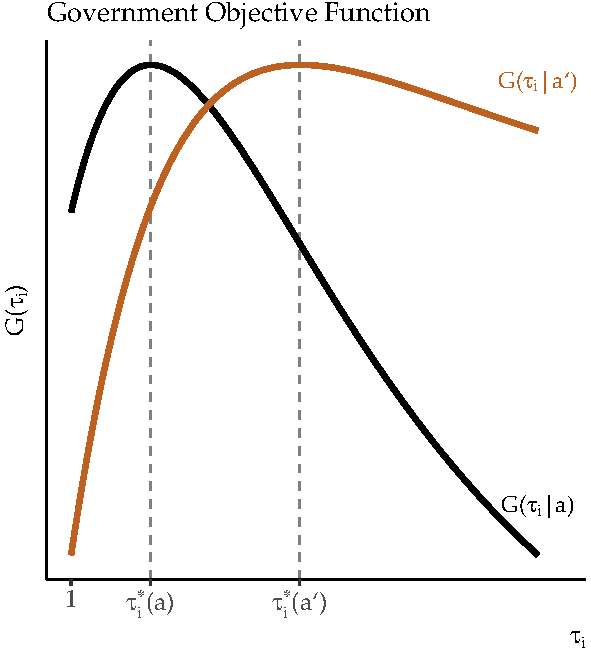
\includegraphics{figure/G-1.pdf}
\caption{Government preferences over own tariff rates with
\(a > a^\prime\) \label{fig:G}}
\end{figure}

Figure \ref{fig:G} depicts the governments' objective functions as a
function of their own tariff choice, \(\tau_i\). As the government
becomes more representative, the peak of the curve shifts to the left,
indicating that the government prefers a lower tariff. This is a natural
result. As the government becomes more representative, it values the
welfare of the consumer more and more. This pushes the government to
adopt a policy that is closer to the consumer's ideal.

\begin{figure}
\centering
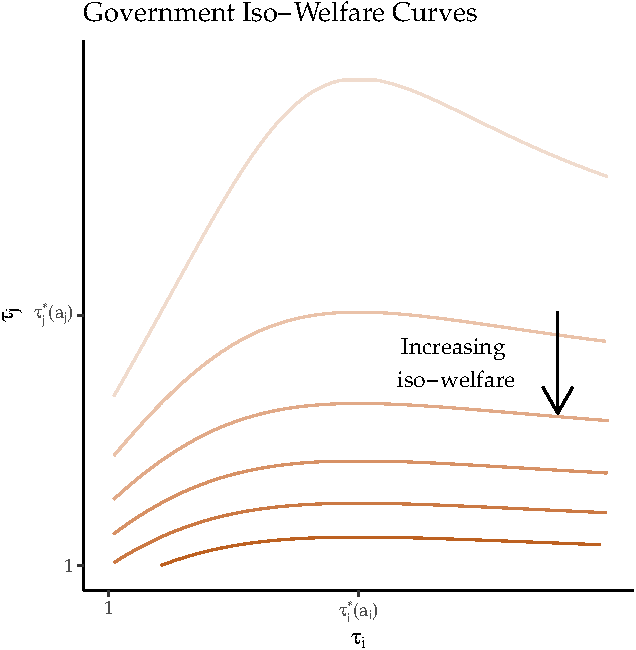
\includegraphics{figure/iso-1.pdf}
\caption{Government iso-welfare curve over home and foreign tariff rates
\label{fig:iso}}
\end{figure}

Figure \ref{fig:iso} depicts the government's welfare in
\(\left( \tau_i, \tau_j \right)\) space. By decreasing the market access
afforded to firms in \(i\), non-zero tariffs in \(j\) strictly decrease
the government's welfare. For any given \(\tau_i\), the government's
welfare is increasing as \(\tau_j\) decreases.

\textbf{Lemma 2:} \(G_i(\tau_j)\) is strictly decreasing in \(\tau_j\).

If the governments were prohibited from bargaining, they would each
simply choose the policy that maximized their utility, taking the other
country's policy choice as given.

\textbf{Definition 3:} A \emph{noncooperative equilibrium} is a pair of
policies \(\left( \tau_i^\star(a_i), \tau_j^\star(a_j) \right)\) such
that \[
\tau_i^\star(a_i) = \argmax_{\tau_i \in [1, \bar{\tau}]} G_i(\tau_i; a_i)
\] and \[
\tau_j^\star(a_j) = \argmax_{\tau_j \in [1, \bar{\tau}]} G_j(\tau_j; a_j) .
\]

Our next result shows that as governments become more liberal, their
optimal tariffs fall.

\textbf{Lemma 3:} \(\tau_i^\star(a_i)\) is strictly decreasing in
\(a_i\).

\begin{figure}
\centering
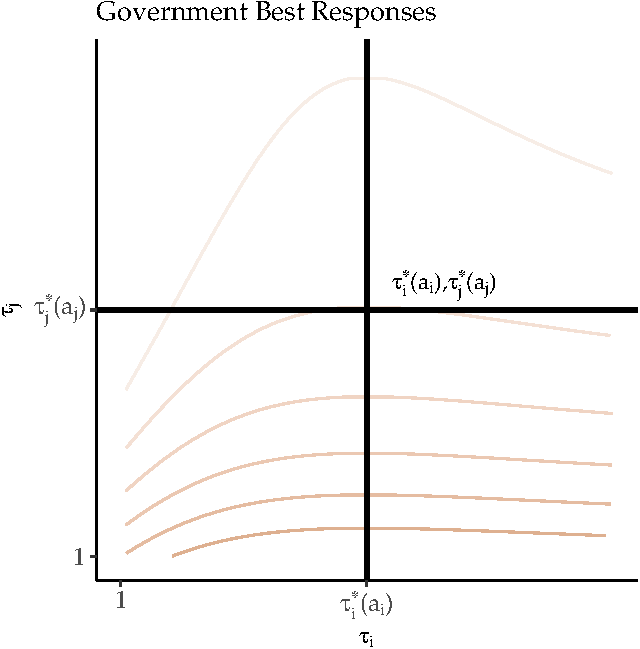
\includegraphics{figure/br-1.pdf}
\caption{Government best response functions \label{fig:br}}
\end{figure}

Figure \ref{fig:br} depicts each governments' best response curves
through the policy space. Because the governments' optimal choices do
not depend on one another's policy choice, their best response curves
are straight lines. Their intersection constitutes the noncooperative
equilibrium. As the governments' preferences become more biased, these
curves shift outward, resulting in a more autarkic noncooperative
equilibrium.

\subsection{Regime Change}

It is now clear that each government cares indirectly about the
preferences of its bargaining partner. More welfare-conscious
governments adopt lower barriers to trade (Lemma 3) in a non-cooperative
equilibrium, which benefits governments abroad by providing greater
market access to their firms. If each government were able to choose the
preferences of their negotiating partner, they would do so in order to
minimize trade barriers. This is the purpose of regime change in this
model. If a government wins a war, it earns the right to replace the
government with a puppet with more ``dovish'' preferences. Regime change
is therefore used instrumentally to pry open international markets. Let
\(a^\star \in (\ubar{a}, \bar{a}]\) denote the type of the optimal
puppet government.

The optimal puppet's type solves \[
\max_{a_j \in (\ubar{a}, \bar{a}]} G_i( \tau_i^\star(a_i), \tau_j^\star(a_j); a_i ) .
\]

\textbf{Proposition 2:} \(a^\star = \bar{a}\) .

If a government wins a war, it will replace the vanquished government
with a maximally-responsive puppet. This government will adopt no trade
barriers, providing maximal market access for the victorious country's
firms. This is the threat point that governments leverage in
international coercive bargaining.

\subsection{Conflicts of Interest}

If a government wins a war it adopts its optimal policy and enjoys
complete access to the markets of its trading partner. This best case
scenario yields the government utility \begin{equation*} \label{eq:Gbar}
\bar{G}_i(a_i) = G_i(\tau_i^\star(a_i), \tau_j^\star(\bar{a}); a_i) .
\end{equation*}

If a government loses a war, it is replaced by a puppet and must suffer
under the policies implemented by the puppet regime. This is consistent
with a notion of the government as a particular amalgamation of social
actors that continues to exist at the conclusion of a war. The
vanquished government yields utility \begin{equation*} \label{eq:Gubar}
\ubar{G}_i(a_i, a_j) = G_i(\tau_i^\star(\bar{a}), \tau_j^\star(a_j); a_i) .
\end{equation*}

These outcomes represent upper and lower utility bounds on the outcome
of any coercive negotiation. Each government can be made no worse off
than if it were to lose a war. And each government can secure no better
bargaining outcome than if they were to (costlessly) win a war for
regime change. The welfare difference between these two scenarios is
taken to be \(i\)'s \emph{conflict of interest} with \(j\). Note that
this conflict of interest, unlike standard models of bargaining and war,
need not be symmetric. The ``pie'' at stake in the negotiation over
trade policies may be valued differently by each government --- \(i\)'s
preference intensity may be stronger than \(j\)'s or vice versa. This
variation in preference intensity, combined with variable military
power, determines bargaining outcomes.

\textbf{Definition 4:} The magnitude of government \(i\)'s
\emph{conflict of interest} with government \(j\) is
\begin{equation} \label{eq:Gamma}
\Gamma_i(a_i, a_j) = \bar{G}_i(a_i) - \ubar{G}_i(a_i, a_j) .
\end{equation}

\textbf{Proposition 3:} \(\Gamma_i(a_i, a_j)\) is decreasing in \(a_i\)
and \(a_j\) .

Proposition 3 states that as government \(i\) becomes more
welfare-conscious, the magnitude of its conflict of interest decreases.
Likewise, as government \(j\) becomes more welfare-conscious, \(i\)'s
conflict of interest with it decreases. As government \(i\) becomes more
welfare-conscious, it prefers less protectionism. This decreases the
difference between \(i\)'s ideal policy and the (free trading) policy
that will be imposed upon it if \(j\) is victorious in a war. As \(j\)
becomes more welfare-conscious, it imposes smaller market access
externalities on \(i\). Regime change becomes relatively less appealing,
because the distance between \(j\)'s preferred policy and the policy
that a puppet would impose shrinks. In the corner case where
\(a_i = a_j = \bar{a}\), the conflict of interest evaporates -- puppets
would implement the exact same policies as the sitting governments.

\subsection{Bargaining}

These conflicts of interest structure what sets of policies \(i\) will
offer and what offers \(j\) will prefer to war. Working backward, recall
from Definition 1 that
\(\omega^\star(\tilde{\bm{\tau}}; a_j, c_j, \rho)\) is a function that
takes an offer from \(i\) and returns a choice of whether or not to
declare war. \(j\)'s utility for war is given by
\begin{equation*} \label{eq:Ghatj}
\hat{G}_j(a_j, a_i) = \underbrace{(1 - \rho) \bar{G}_j(a_j) + \rho \ubar{G}_j(a_j, a_i)}_{W_j(a_j, a_i)} - c_j = (1 - \rho) \Gamma_j(a_j, a_i) + \ubar{G}_j(a_j, a_i) - c_j .
\end{equation*}

Note that \(j\)'s utility can be written in terms of its conflict of
interest with \(i\). \(j\) will prefer war to \(i\)'s offer whenever \[
\hat{G}_j(a_j, a_i) \geq G_j(\tilde{\bm{\tau}}; a_j) .
\] This condition allows us to characterize
\(\omega^\star(\tilde{\bm{\tau}}; a_j, c_j, \rho)\).

\textbf{Lemma 4:} \[
\omega^\star(\tilde{\bm{\tau}}; a_j, c_j, \rho) = \begin{cases}
\text{war} & \text{if } \hat{G}_j(a_j, a_i) \geq G_j(\tilde{\bm{\tau}}; a_j) \\
\text{accept} & \text{otherwise}
\end{cases}
\]

If \(j\)'s conflict of interest with \(i\) is small enough, then \(i\)
can simply offer its ideal point and all cost types of \(j\) will
accept.

\textbf{Lemma 5:} If \[
W_j(a_j, a_i) - G_j(\tau_j^\star(\bar{a}), \tau_i^\star(a_i); a_j) = \Gamma_j(a_j, a_i) \leq \ubar{c}_j
\] then \[
\tilde{\bm{\tau}}^\star = \left( \tau_i^\star(a_i), \tau_i^\star(\bar{a}) \right)
\] and \[
\omega^\star(\tau_i^\star(a_i), \tau_j^\star(\bar{a}); a_j, c_j, \rho) = \text{accept}
\] for all \(c_j \in [\ubar{c}_j, \bar{c}_j]\).

Given our assumptions on the costs of war, we can always find a cutpoint
bias type for the foreign country such that all types more liberal than
the cutpoint accept \(i\)'s ideal point.

\textbf{Lemma 6 (Zone of Peace):} For every
\(\ubar{c}_j \in [ 0, \bar{c}_j )\) there exists a
\(a_j(\ubar{c}_j, a_i)\) such that for all
\(a_j \in [ a_j(\ubar{c}_j, a_i), \bar{a} )\) the probability of war is
0.

Lemma 6 proves the existence of a ``Zone of Peace'' -- a set of foreign
bias types that never fight in equilibrium. Combining this observation
with the fact that \(j\)'s conflict of interest with \(i\) is decreasing
in \(i\)'s bias type yields our first core result. Namely, that the size
of this zone of peace is increasing as \(i\) becomes more liberal in its
policy preferences. Figure \ref{fig:zop} depicts this result.

\begin{figure}
\centering
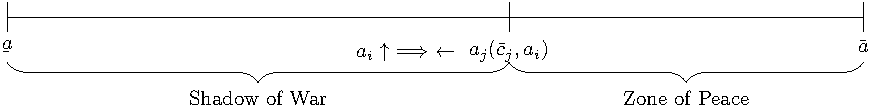
\includegraphics{figure/aLine.pdf}
\caption{As the home government becomes more liberal, the set of foreign
types that accept its ideal point expands. \label{fig:zop}}
\end{figure}

\textbf{Proposition 4 (Liberal Peace):} \(a_j(\ubar{c}_j, a_i)\) is
weakly decreasing in \(a_i\).

Whenever \(a_j \geq a_j(\ubar{c}_j, a_i)\), \(i\) offers its ideal point
which is accepted by \(j\). This guarantees peace. \(j\) is more willing
to accept \(i\)'s ideal point as it becomes more liberal, because
\(i\)'s ideal policy imposes smaller and smaller externalities on \(j\).
This generates a ``Liberal Peace.'' When peace prevails, liberal
governments also settle on more open trade policy regimes overall.
Naturally, reducing trade costs increases trade between the governments.

\textbf{Proposition 5 (Liberal Trade):} If
\(a_j \geq a_j(\ubar{c}_j, a_i)\) then trade in manufactured goods is
increasing in \(a_i\).

If \(a_j < a_j(\ubar{c}_j, a_i)\), however, then \(i\) faces a
risk-return tradeoff (Powell 1999). Offers closer to \(i\)'s ideal point
yield higher utility conditional on acceptance, but also generate a
higher risk of war. Here, the shadow of power affects equilibrium
policies.

For any offer, the probability that \(j\) will declare war is given by
\begin{equation} \label{eq:prwar}
\begin{split}
\text{Pr} \left( c_j \leq W_j(a_j, a_i) - G_j(\tilde{\bm{\tau}}; a_j) | \tilde{\bm{\tau}}, a_i, a_j \right) = F \left( W_j(a_j, a_i) - G_j(\tilde{\bm{\tau}}; a_j)  \right) .
\end{split}
\end{equation}

With this quantity known, we can work to characterize \(i\)'s offer
function, \(\tilde{\bm{\tau}}^\star(a_i)\). If war occurs, \(i\)
receives utility \begin{equation*} \label{eq:Ghati}
\hat{G}_i(a_i, a_j) = \rho \Gamma_i(a_i, a_j) + \ubar{G}_i(a_i, a_j) - c_i .
\end{equation*}

With the probability of war given in Equation \ref{eq:prwar}, we can
write \(i\)'s utility for any offer as
\begin{equation} \label{eq:Gtildei}
\begin{split}
\tilde{G}_i \left( \tilde{\bm{\tau}}, \omega^\star(\tilde{\bm{\tau}}; a_j, c_j, \rho); a_i, c_i, \rho \right) = \underbrace{\left( 1 - F \left( W_j(a_j, a_i) - G_j( \tilde{\bm{\tau}}; a_j ) \right) \right) \left( G_i( \tilde{\bm{\tau}}; a_i ) \right)}_{\neg \text{war}} + \\
\underbrace{F \left( W_j(a_j, a_i) - G_j(\tilde{\bm{\tau}}; a_j) \right) \left( \hat{G}_i(a_i, a_j) \right)}_{\text{war}} .
\end{split}
\end{equation}

By Definition 1, \(i\)'s equilibrium offer will maximize this objective
function. Lemmas \texttt{7} and \texttt{8} state that an offer will lie
inside the pareto set and that proposed trade policies will be weakly
more liberal than those in a noncooperative equilibrium (Definition 3).

\textbf{Definition 5:} The \emph{pareto set} is given by \[
\mathcal{P} = \left\{ \tilde{\bm{\tau}} \in [1, \bar{\tau}]^2 | \tilde{\bm{\tau}} \in \argmax_{\tilde{\bm{\tau}} \in [1, \bar{\tau}]^2} \lambda G_i(\tilde{\bm{\tau}}; a_i) + (1 - \lambda) G_j(\tilde{\bm{\tau}}; a_j) \right\}
\] for some \(\lambda \in [0, 1]\).

\textbf{Lemma 7:}
\(\tilde{\bm{\tau}}^\star(a_i, c_i, \rho) \in \mathcal{P}\) .

\textbf{Lemma 8:}
\(\tilde{\bm{\tau}} = \left( \tilde{\tau}_i^\star, \tilde{\tau}_j^\star \right) \leq \left( \tau_i^\star(a_i, c_i, \rho), \tau_j^\star(a_i, c_i, \rho) \right)\)
with \(\leq\) the natural vector order.

These Lemmas establish that any policy proposal is efficient and that
tariffs are weakly lower than those in the noncooperative equilibrium.
How \(i\) chooses to resolve the risk-return tradeoff depends on its
military power. Relatively powerful governments can implement their
ideal point with high probability through war. They run little risk that
the foreign government would reject an offer close to their ideal point.
Conversely, weak governments are likely to lose a war over market
access, and therefore must concede more to their counterpart. Military
power therefore affects trade policy. Because \(i\)'s ideal point
features more protection of its own market than \(j\)'s ideal point, as
\(i\) becomes more powerful, it proposes higher levels of protection for
itself. If this offer is accepted and peace prevails, powerful countries
will be more closed to international trade.

\textbf{Proposition 6 (Power and Protection):} If
\(a_j < a_j(\ubar{c}_j, a_i)\) and peace prevails, government \(i\)'s
trade barriers are increasing in its military strength,
i.e.~\(\tilde{\tau}_i^\star(a_i, c_i, \rho)\) is increasing in \(\rho\).

\section{Discussion}

Jointly, Propositions 4 and 5 establish that the most liberal
governments never fight and also trade more than illiberal governments.
Contra the commercial peace framework, trade is endogenously determined
by governments trade policy choices. These endogenous trade policies
determine trade flows and generate conflicts between governments.
Economic integration is not exogenously given. Rather, participation in
the international economy is a choice. Even in today's globalized era,
such policy frictions persist (Anderson and Van Wincoop 2004; Cooley
2019a).

These policy choices are the object of contention between governments in
the model. Protectionist barriers cause conflicts of interest between
market access-motivated governments. McDonald (2004) shows that measures
of protection are better predictors of conflict than trade.\footnote{His
  analysis covers the years 1960-2000.} Trade can persist in the
presence of trade barriers. For example, World War I broke out during an
era of rapid globalization. McDonald and Sweeney (2007) show that the
great powers maintained high protective tariffs during this era, which
provided a rationale for conflict over market access conditions, despite
high trade volumes. Chatagnier and Kavakli (2015) examine governments
whose firms compete in the same export markets. They show these
governments are more likely to experience international conflicts.

Firms are the source of belligerent foreign policies in the theory. In
Imperial Germany, ``iron and rye'' advocated for protectionism and
expansionist foreign policies (Gerschenkron 1943). Similar domestic
political coalitions emerged in the United States. Fordham (2019) traces
the development of the United States as a naval power in the 19th
century. He finds protectionist interests were the strongest advocates
for the nascent U.S. fleet. At the time, U.S. trade policy was
protectionist. Washington also sought preferential market access in
developing countries, particularly in Latin America. The fleet served to
protect these objectives against military interference from Europe.
Commercial objectives also motivated Washington at the dawn of the Cold
War (Fordham 1998). Under Soviet influence, Eastern Europe became closed
to trade with the United States. Congressmen representing
export-oriented districts tended to support an aggressive military
posture toward the Soviet Union. The goal of export-oriented firms,
argues Fordham, was to secure market access in Europe and Japan. In the
post-Cold War era, Congressmen representing import-exposed districts
have tended to support hostile foreign policies toward China, whose
exports (plausibly) harm their constituent firms (Kleinberg and Fordham
2013).

Domestic political institutions connect these underlying economic
interests to government preferences. I treat these institutions in
reduced form, focusing on variation in consumers' ability to influence
policy. Consumers pacify foreign policy preferences. If democratic
political institutions privilege the interests of consumers, then
Propositions 4 and 5 support a commercial-democratic peace.
Observational analyses uncover positive correlations between democracy,
trade, and peace because of the trade policy preferences of
democracies.\footnote{See Oneal and Russett (1999) for a representative
  study.} Liberal preferences increase trade and reduce conflict.

Observed trade policies are not a sufficient statistic for government
preferences, however. Proposition 6 states that relative military power
effects trade policy in peacetime. Governments' trade policies reflect
their preferences only up to a war constraint. Liberal \emph{policies}
do not imply liberal \emph{preferences}. Several studies have employed
Grossman and Helpman (1994) and Grossman and Helpman (1995) to
structurally estimate governments' welfare-consciousness (Goldberg and
Maggi 1999; Mitra, Thomakos, and Ulubasoglu 2006; Gawande, Krishna, and
Olarreaga 2009, 2012, 2015; Ossa 2014). International strategic
considerations are effectively absent from these models. The domestic
political economy determines outcomes. Therefore, a simple inversion on
the policy function recovers preferences. The model developed here
highlights the importance of the war constraint. Militarily weak,
illiberal governments adopt the same policies as liberal governments.

Territory plays a central role in theories and empirical studies of
interstate conflict.\footnote{The ``pie'' at stake in bargaining models
  of war is often motivated as the distribution of territory between the
  countries. Empirical studies of territorial conflict often
  conceptualize territorial control as a consumption good, rather than a
  means to implement policy. See, for example, Caselli, Morelli, and
  Rohner (2015). For a review of this literature, see Schultz (2015).}
Wars often redraw international borders. In doing so, they also relocate
customs barriers and modify the trade policies of captured regions.
Gunboat diplomacy and territorial conflict are plausibly substitutes for
one another. Governments can acquire foreign market access through
territorial annexation or regime change. Territory and trade policy are
not exclusive realms of international conflict.

\section{Conclusion}

The model envisions a stylized world. Two governments preside over
identical economies exogenous military capacities and political bias
types. If the countries were heterogeneous in market size (\(L_i\)), the
economically larger country would possess an additional source of
bargaining power. Whether this outside option affects bargaining
outcomes would depend on the distribution of economic and military
strength. This analysis might shed light the substitutability of
economic and military coercion (Hirschman 1945).

Military power (\(\rho\)) is also treated as exogenous here. If military
investment was possible, \(\rho\) would depend on economic and political
primitives.\footnote{See, for example, Jackson and Morelli (2009a).}
Because they have more at stake in bargaining, illiberal governments
might invest more in their militaries. This result would hold especially
if the costs of militarization are borne by consumers (Jackson and
Morelli 2007; Chapman, McDonald, and Moser 2015). This variant might
explain why democracies spend less on their militaries (Fordham and
Walker 2005).

If the game developed here was dynamic, regime type itself would be an
endogenous object. Wars impose puppet governments more liberal than
those that preceded them. The world would democratize over time, as
conquering powers installed liberal governments abroad. (McDonald 2015).

While imperial powers sometimes seek to democratize defeated countries,
they often instead install allied strongmen or colonial administrations.
If the liberal democracy hypothesis holds, these actions are puzzling.
Controlling these governments presents agency problems absent in
relations with liberal regimes. Liberal regimes adopt liberal trade
policies of their own accord. Conquerors must incentivize their agents
to adopt these policies.

A multi-country variant of this framework might provide a rationale for
this behavior. Consider a world populated with three countries --- A, B,
and C. For firms in A, an ideal policy for B is one that is open to
trade with A but closed to trade from C. This allows A's firms to
maximize their share of B's market.\footnote{This assumes, of course,
  that B cannot tax its own firms.} In other words, firms seek
\emph{preferential} access to foreign markets. It is immediate that a
low bias government would not provide such preferential access. Coercing
governments might be willing to suffer the agency costs of obtaining
preferential access to B if B's market was valuable enough. This
framework might be profitably applied to the study of imperialism
(Gallagher and Robinson 1953).

Finally, the theory highlights an underappreciated prerequisite for
international conflict. For governments to war with one another, they
must both 1) possess conflicts of interest large enough to justify the
costs of conflict and 2) be unable to resolve these conflicts peacefully
(Jackson and Morelli 2009b). Theoretical research on international
conflict has focused on the latter. In abstracting away from the exact
nature of the dispute at hand, these models direct our attention away
from the question of why international disputes emerge in the first
place. What do governments want, and why do their objectives bring them
into conflict with one another (Moravcsik 1997; Coe, n.d.)? While war is
rare in international politics, antagonistic and militarized political
relations are common. Focusing attention on the conflicts of interest
underlying these antagonisms might help explain their emergence and
termination.

\clearpage

\section{Appendix}

\subsection{A: Trade, War, and Democracy: Empirical Facts}

\begin{figure}
\centering
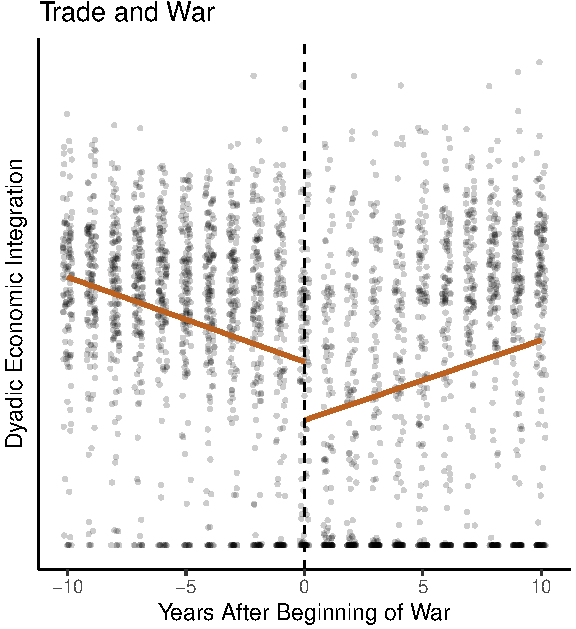
\includegraphics{figure/tradeRD-1.pdf}
\caption{Plot depicts trade relations between dyads that experienced
wars, 10 years prior to and 10 years following the outbreak of
hostilities. Economic integration is measured as the average of the
countries' directed imports to gdp ratio. An inverse hyperbolic sine
transformation was applied to normalize this measure. Data from
Barbieri, Keshk, and Pollins (2008), Barbieri, Keshk, and Pollins
(2009), Sarkees and Wayman (2010), Bolt et al. (2018).
\label{fig:tradeRD}}
\end{figure}

\begin{figure}
\centering
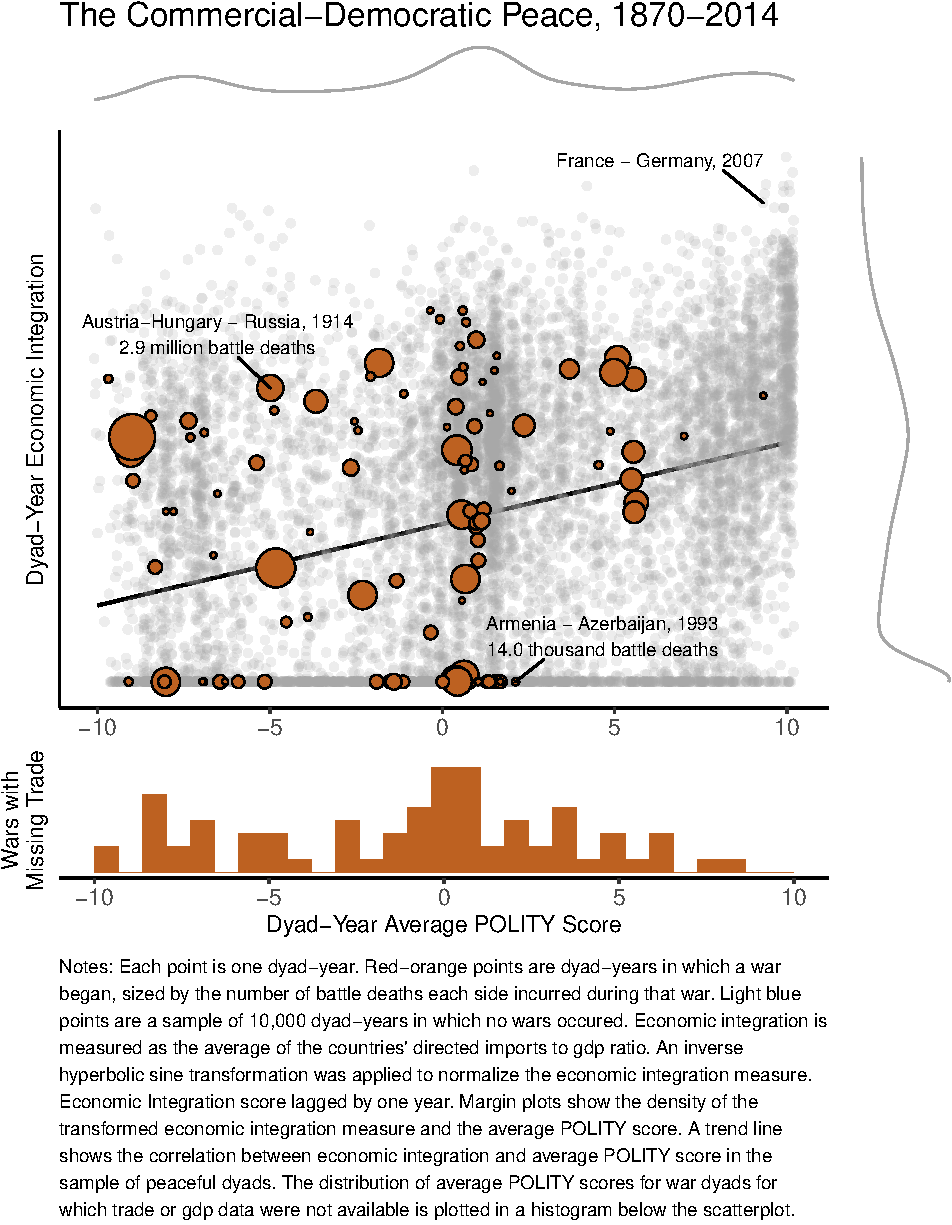
\includegraphics{figure/comdempeace-1.pdf}
\caption{Data from Marshall, Jaggers, and Gurr (2002), Barbieri, Keshk,
and Pollins (2008), Barbieri, Keshk, and Pollins (2009), Sarkees and
Wayman (2010), Bolt et al. (2018). \label{fig:comdempeace}}
\end{figure}

\clearpage

\subsection{B: International Economy}

\textbf{Demand for Manufactured Goods:} Total expenditure on
manufactured goods is \(\alpha I_i = P_i X_i\). Cobb Douglas preferences
ensure that consumers will spend an \(\alpha\)-share of their income on
manufactured goods. We can derive Equation \ref{eq:demand} by solving
Equation \ref{eq:CES} subject to the constraint
\begin{equation} \label{eq:CESconstraint}
\int_{\nu_i} p_{ii}(\nu_i) x_{ii}(\nu_i) d \nu_i + \int_{\nu_j} p_{ij}(\nu_j) x_{ij}(\nu_j) \leq \alpha w_i L .
\end{equation} For any two domestic varieties, \(\nu_i\) and
\(\nu_i^\prime\), we must have \begin{align*}
x_{ii}^\star(\nu_i) p_{ii}(\nu_i)^{\sigma} p_{ii}(\nu_i^\prime)^{1 - \sigma} &= p_{ii}(\nu_i^\prime) x_{ii}^\star(\nu_i^\prime) \\
x_{ii}^\star(\nu_i) p_{ii}(\nu_i)^{\sigma} \int_{\nu_i^\prime} p_{ii}(\nu_i^\prime)^{1 - \sigma} d \nu_i^\prime &= \int_{\nu_i^\prime} p_{ii}(\nu_i^\prime) x_{ii}^\star(\nu_i^\prime) d \nu_i^\prime .
\end{align*}

The same must hold for foreign varieties: \[
x_{ij}^\star(\nu_j) p_{ij}(\nu_j)^{\sigma} \int_{\nu_j^\prime} p_{ij}(\nu_j^\prime)^{1 - \sigma} d \nu_j^\prime = \int_{\nu_j^\prime} p_{ij}(\nu_j^\prime) x_{ij}^\star(\nu_j^\prime) d \nu_j^\prime .
\] Summing these conditions and noting
\(x_{ij}^\star(\nu_j) p_{ij}(\nu_j)^{\sigma} = x_{ii}^\star(\nu_i) p_{ii}(\nu_i)^{\sigma}\)
at equilibrium consumption gives \begin{align*}
x_{ii}^\star(\nu_i) p_{ii}(\nu_i)^{\sigma} \left( \int_{\nu_i^\prime} p_{ii}(\nu_i^\prime)^{1 - \sigma} d \nu_i^\prime + \int_{\nu_j^\prime} p_{ij}(\nu_j^\prime)^{1 - \sigma} d \nu_j^\prime \right) &= \int_{\nu_i^\prime} p_{ii}(\nu_i^\prime) x_{ii}^\star(\nu_i^\prime) d \nu_i^\prime + \int_{\nu_j^\prime} p_{ij}(\nu_j^\prime) x_{ij}^\star(\nu_j^\prime) d \nu_j^\prime \\
x_{ii}^\star(\nu_i) p_{ii}(\nu_i)^{\sigma} P_i(\tau_i)^{1 - \sigma} &= \alpha I_i(\tau_i) \\
x_{ii}^\star(\nu_i) &= p_{ii}(\nu_i)^{-\sigma} P_i(\tau_i)^{\sigma - 1} \alpha I_i(\tau_i) .
\end{align*}

\textbf{Indirect Utility:} Indirect utility is \(X_i^\alpha Y_i^\alpha\)
evaluated at equilibrium consumption. Substituting our demand equations
\ref{eq:demand} into Equation \ref{eq:CES} gives \begin{align*}
X_i^\star &= \left( \int_{\nu_i} x_{ii}^\star(\nu_i)^{\frac{\sigma - 1}{\sigma}} d \nu_i + \int_{\nu_j} x_{ij}^\star(\nu_j)^{\frac{\sigma - 1}{\sigma}} d \nu_j \right)^{\frac{\sigma}{\sigma - 1}} \\
&= P_i(\tau_i)^{\sigma - 1} I_i(\tau_i) \left( \int_{\nu_i} p_{ii}(\nu_i)^{1 - \sigma} + p_{ij}(\nu_j)^{1 - \sigma} \right)^{\frac{\sigma}{\sigma - 1}} \\
&= \alpha \frac{I_i(\tau_i)}{P_i(\tau_i)} .
\end{align*}

Because they serve as numeraire, equilibrium consumption of agricultural
goods is equivalent to expenditure:
\(Y_i^\star = (1 - \alpha) I_i(\tau_i)\). Substituting these into the
consumer's utility function yields Equation \ref{eq:V}.

\textbf{Prices:} The firms' first order condition is \[
\frac{\partial \Pi \left( p_i^\star(\nu_i) \right)}{\partial p_i^\star(\nu_i)} = \left( p_i^\star(\nu_i) - w_i \right) \left( \frac{\partial x_{ii}^\star(\nu_i)}{\partial p_i^\star(\nu_i)} + \frac{\partial x_{ji}(\nu_i)}{\partial p_i^\star(\nu_i)} \right) + x_{ii}^\star(\nu_i) + x_{ji}^\star(\nu_i) = 0
\] where \[
\frac{\partial x_{ii}(\nu_i)}{\partial p_i(\nu_i)} = - \sigma p_i^(\nu_i)^{- \sigma - 1} P_i^{\sigma - 1} \alpha I_i
\] and \[
\frac{\partial x_{ji}(\nu_i)}{\partial p_i(\nu_i)} = - \sigma \tau_j^{-\sigma} p_i^(\nu_i)^{- \sigma - 1} P_j^{\sigma - 1} \alpha I_i .
\] Note that \[
- \frac{\sigma}{p_i^\star(\nu_i)} \left( x_{ii}^\star(\nu_i) + x_{ji}^\star(\nu_i) \right) = \frac{\partial x_{ii}(\nu_i)}{\partial p_i^\star(\nu_i)} + \frac{\partial x_{ji}(\nu_i)}{\partial p_i^\star(\nu_i)} .
\] The first order condition then becomes \begin{align*}
\sigma \frac{w_i}{p_i^\star(\nu_i)} \left( x_{ii}^\star(\nu_i) + x_{ji}^\star(\nu_i) \right) - \sigma \left( x_{ii}^\star(\nu_i) + x_{ji}^\star(\nu_i) \right) + \left( x_{ii}^\star(\nu_i) + x_{ji}^\star(\nu_i) \right) &= 0 \\
\sigma \frac{w_i}{p_i^\star(\nu_i)} - \sigma + 1 &= 0 \\
\frac{\sigma}{\sigma - 1} w_i &=  p_i^\star(\nu_i) .
\end{align*}

\textbf{Economic Equilibrium:}

With unit costs of production in manufacturing and agriculture, goods
market clearing requires \begin{equation*}
\begin{split}
L_i^y + L_j^y = (1 - \alpha) \left( I_i(\tau_i) + I_j(\tau_j) \right) \\
L_i^x = \left( x_{ii}^\star(\tau_i) + x_{ji}^\star(\tau_j) \right) \\
L_j^x = \left( x_{ij}^\star(\tau_i) + x_{jj}^\star(\tau_j) \right) \\
L_i^x + L_j^x + \Pi_i(p_i^\star) + \Pi_j(p_j^\star) = \alpha \left( I_i(\tau_i) + I_j(\tau_j) \right) .
\end{split}
\end{equation*}

Domestic factor market clearing requires \begin{equation*}
\begin{split}
L_i^x + L_i^y = L \\
L_j^x + L_j^y = L .
\end{split}
\end{equation*}

\subsection{C: Constant Definitions}

\textbf{Assumption 1}

I restrict \(j\)'s costs of war such that there exists some government
\(j\) with \(a_j \in (\ubar{a}, \bar{a}]\) that would be willing to
fight if victory were certain and \(i\) offered its ideal point.
Formally, this requires \[
\kappa_j = \Gamma_j(\ubar{a}, a_i) .
\] I then restrict \(i\)'s costs of war to ensure that it never offers
\(j\)'s ideal point -- an interior solution exists outside of the zone
of peace. Formally, this requires \[
\kappa_i(\bar{c}_j, a_i) = \min_{\tilde{\bm{\tau}} \in \mathcal{P}} - \bar{c}_j \left( 1 - F \left( W_j(\ubar{a}, a_i) - G_j(\cdot, \tilde{\tau}_i; a_j) \right) \right) \frac{ \frac{\partial G_i(\tau_i, \cdot; a_i)}{\partial \tau_i} }{ \frac{\partial G_j(\cdot, \tau_i; a_i)}{\partial \tau_i} } .
\] Because
\(\frac{\partial G_j(\cdot, \tau_i; a_i)}{\partial \tau_i} < 0\), this
quantity is guaranteed to be positive.

\textbf{Assumption 3}

Let \[
\ubar{a} = (\sigma - 1) k(\alpha)^{-1} (p^\star)^{\alpha} (1 - (p^\star)^{-1})
\] where \[
k(\alpha) = \alpha^\alpha (1 - \alpha)^{1 - \alpha} .
\] This quantity is derived by letting \[
\ubar{a} = \left\{ a_i \,\middle|\, \lim_{\tau_i \rightarrow \infty} a_i V_i^\prime(\tau_i) + \Pi_i^\prime(\tau_i) = 0 \right\} .
\] Note that it is positive.

\subsection{D: Proofs}

Restatements of results from the main text proceed all proofs. Lemmas 2,
and 3 exploit the following definitions: \[
A(\tau_i) = p^\star x_{ij}^\star(\tau_i) (\alpha I(\tau_i))^{-1} = \left( 1 + \tau_i^{1-\sigma} \right)^{-1} \tau_i^{-\sigma}
\] \[
B(\tau_i) = (\sigma - 1) A(\tau_i) - \sigma \tau_i^{-1} .
\]

\textbf{Proposition 1:} If Assumption 2 is satisfied, then a unique
economic equilibrium exists with \(L_i^x, L_i^y, L_j^x, L_j^y > 0\) and
\(w_i = w_j = 1\) for all \(\bm{\tau} \in [1, \bar{\tau}]^2\).

\textbf{Proof:} A competitive agricultural sector guarantees that
agricultural producers make zero profits. This zero profit condition
implies \[
\left( 1 - w_i \right) Y_i = 0
\] which implies \(w_i = 1\) whenever the agricultural sector is active,
\(Y_i > 0\). From Equation \ref{eq:prices}, this implies
\(p_i^\star = p_j^\star = p^\star = \frac{\sigma}{\sigma - 1}\). Suppose
for now that the agricultural sector is active in both countries,
implying wages are equalized across countries and sectors. Below, we
verify that this is the case if Assumption 2 is satisfied.

Labor allocations to each sector depend on tariff levels. The labor
allocation in country \(i\) to sector \(k \in \left\{ x, y \right\}\)
can then be written \(L_i^k(\bm{\tau})\). The total labor allocation to
the manufacturing sector in country \(i\) is \[
L_i^x(\bm{\tau}) = x_{ii}^\star(\tau_i) + x_{ji}^\star(\tau_j) .
\] Because \(x_{ii}^\star(\tau_i)\) is increasing in \(\tau_i\) and
\(x_{ji}^\star(\tau_j)\) is decreasing in \(\tau_j\) (see Lemma 2.),
\(L_i^x(\bm{\tau})\) is monotone increasing in \(\tau_i\) and monotone
decreasing in \(\tau_j\). This implies \(L_i^x(\bm{\tau})\) attains its
maximum at \(\left( \bar{\tau}, 1 \right)\):\footnote{Here we note the
  dependence of the price index on the home tariff \(P_i(\tau_i)\).}
\begin{align*}
L_i^x(\bar{\tau}, 1) &= p^{-\sigma} P_i(\bar{\tau})^{\sigma - 1} \alpha L + (1 p)^{-\sigma} P_j(1)^{\sigma - 1} \alpha L \\
&= \frac{p^{-\sigma} \alpha L}{p^{1 - \sigma}} + \frac{p^{-\sigma} \alpha L}{2 p^{1 - \sigma}} \\
&= \frac{\alpha L}{p} + \frac{1}{2} \frac{\alpha L}{p} \\
&= \frac{3}{2} \frac{\sigma - 1}{\sigma} \alpha L .
\end{align*} Allocation to the agricultural sector is then, by the labor
market clearing condition, \[
L_i^y(\bar{\tau}, 1) = L - L_i^x(\bar{\tau}, 1) .
\] If \(\alpha < \frac{2}{3} \frac{\sigma}{\sigma - 1}\), then
\(L_i^y(\bar{\tau}, 1) > 0\). Because total labor allocation to the
manufacturing sector achieves its maximum at
\(\left( \bar{\tau}, 1 \right)\), \(L_i^y(\bm{\tau}) > 0\) for all
\(\bm{\tau} \in [1, \bar{\tau}]^2\). Moreover, \(L_i^x(\bm{\tau}) > 0\)
for all \(\bm{\tau} \in [1, \bar{\tau}]^2\).\footnote{This follows from
  the fact that \(L_i^x(1, \bar{\tau}) > 0\) and the monotonicities
  established above.} This demonstrates the proposition.
\(\blacksquare\)

\textbf{Lemma 1:} \(\tau_i^\star(a_i) \in (1, \bar{\tau})\) .

\textbf{Proof:} The first order condition is
\begin{equation} \label{eq:Gfoc}
0 = - \alpha a_i V_i(\tau_i) A(\tau_i) + a_i r_i^\prime(\tau_i) P_i(\tau_i)^{-\alpha} + \Pi_i^\prime(\tau_i) .
\end{equation}

By construction, \[
\lim_{\tau_i \rightarrow \infty} \frac{\partial G_i}{\partial \tau_i} < 0
\] for all \(a_i > \ubar{a}\). Additionally, \[
\evalat[\Big]{ \frac{\partial G_i}{\partial \tau_i} }{\tau_i=1} = \evalat[\Big]{ \frac{\partial \Pi(\tau_i)}{\partial \tau_i} }{\tau_i=1} > 0 .
\] This precludes \(\tau_i \in \left\{ 1, \bar{\tau} \right\}\) from
being optimal. From each corner point, the directional derivative toward
the interior of the policy space is positive. \(\blacksquare\)

\textbf{Lemma 2:} \(G_i(\tau_j)\) is strictly decreasing in \(\tau_j\).

\textbf{Proof:} It is sufficient to show that \[
\frac{\partial G_i(\tau_j)}{\partial \tau_{j}} < 0 .
\] Note that \[
\frac{\partial G_i(\tau_j)}{\partial \tau_{j}} = \frac{\partial \Pi_i(\tau_i, \tau_j)}{\partial \tau_j} = (p^\star - 1) x_{ji}^{\star \prime}(\tau_j) .
\] The derivative of home exports with respect to the foreign tariff is
\begin{align*}
x_{ji}^{\star \prime}(\tau_j) &= B(\tau_j) x_{ji}^\star(\tau_j) + \frac{x_{ji}^\star(\tau_j)}{I(\tau_j)} r_j^\prime(\tau_j) \\
&= B(\tau_j) x_{ji}^\star(\tau_j) + \frac{x_{ji}^\star(\tau_j)}{I(\tau_j)} \left( (\tau_j - 1) p^\star x_{ji}^{\star \prime}(\tau_j) + p^\star x_{ji}^\star(\tau_j) \right) \\
&= B(\tau_j) x_{ji}^\star(\tau_j) + \frac{x_{ji}^\star(\tau_j)}{I(\tau_j)} \left( \frac{r_j(\tau_j)}{x_{ji}^\star(\tau_j)} x_{ji}^{\star \prime}(\tau_j) + p^\star x_{ji}^\star(\tau_j) \right) \\
&= B(\tau_j) x_{ji}^\star(\tau_j) + \lambda(\tau_j) x_{ji}^{\star \prime}(\tau_j) + p^\star x_{ji}^\star(\tau_j) + \frac{x_{ji}^\star(\tau_j)}{I(\tau_j)} \\
(1 - \lambda(\tau_j)) x_{ji}^{\star \prime}(\tau_j)&= x_{ji}^\star(\tau_j) \left( B(\tau_j) + p^\star x_{ji}^\star(\tau_j) I(\tau_j)^{-1} \right) \\
&= x_{ji}^\star(\tau_j) \left( B(\tau_j) + \alpha A(\tau_j) \right) \\
&< x_{ji}^\star(\tau_j) \left( B(\tau_j) + A(\tau_j) \right) \\
&= \sigma \tau^{-1} \underbrace{\left( \left( 1 + \tau_j^{1-\sigma} \right)^{-1} \tau_j^{-\sigma - 1} - 1 \right)}_{<0} .
\end{align*} \(\blacksquare\)

\textbf{Lemma 3:} \(\tau_i^\star(a_i)\) is strictly decreasing in
\(a_i\).

\textbf{Proof:} Government \(i\)'s optimal policy does not depend on the
policy choice of \(j\). As such, it is sufficient to show that the
government's objective function has a negative cross partial with
respect to \(\tau_i\), \(a_i\), or \[
\frac{\partial^2 G_i}{\partial a_i \partial \tau_{i}} < 0 .
\] This can be written \begin{align*}
\frac{\partial^2 G_i}{\partial a_i \partial \tau_{ij}} &= V_i^\prime(\tau_i) \\
&= r^\prime(\tau_i) P_i(\tau_i)^{\alpha} - \alpha P_i(\tau_i)^{\alpha} I(\tau_i) A(\tau_i) \\
&= \alpha P_i(\tau_i)^{\alpha} I(\tau_i) \left( (\alpha I(\tau_i))^{-1} r^\prime(\tau_i) - A(\tau_i) \right) \\ 
&= \alpha P_i(\tau_i)^{\alpha} I(\tau_i) \left( (\alpha I(\tau_i))^{-1} \left( (\tau_i - 1) p^\star x_{ij}^{\star \prime}(\tau_i) + p^\star x_{ij}^\star(\tau_i) \right) - A(\tau_i) \right) \\
&= P_i(\tau_i)^{\alpha} I(\tau_i) \left( (\alpha I(\tau_i))^{-1} (\tau_i - 1) p^\star x_{ij}^{\star \prime}(\tau_i) + A(\tau)_i - A(\tau_i) \right) \\
&= P_i(\tau_i)^{\alpha} \alpha^{-1} (\tau_i - 1) p^\star \underbrace{x_{ij}^{\star \prime}(\tau_i)}_{<0}
\end{align*} where the final inequality follows from Lemma 2.
\(\blacksquare\)

\textbf{Proposition 2:} \(a^\star = \bar{a}\) .

\textbf{Proof:} Follows immediately from Lemma 2 and Lemma 3.
\(\blacksquare\)

\textbf{Proposition 3:} \(\Gamma_i(a_i, a_j)\) is decreasing in \(a_i\)
and \(a_j\) .

\textbf{Proof: } To establish that \(\Gamma_i(a_i, a_j)\) is decreasing
in \(a_i\), note that derivative of \(\Gamma_i(a_i, a_j)\) taken with
respect to \(a_i\) is \begin{align*}
\frac{\partial \Gamma_i(a_i, a_j)}{\partial a_i} =& \left. \frac{\partial G_i(\tau_i^\star(a_i), \tau_i^\star(\bar{a}); a_i)}{\partial a_i} \right|_{\left( \tau_i^\star(a_i), \tau_j^\star(\bar{a}) \right)} + \underbrace{\frac{\partial G_i(\tau_i^\star(a_i), \tau_j^\star(\bar{a}); a_i)}{\partial \tau_i^\star(a_i)}}_{=0} \frac{\partial \tau_i^\star(a_i)}{\partial a_i} - \\
& \left. \frac{\partial G_i(\tau_i^\star(\bar{a}), \tau_j^\star(a_j); a_i)}{\partial a_i} \right|_{\left( \tau_i^\star(\bar{a}), \tau_j^\star(a_j) \right)} \\
=& \underbrace{V_i(\tau_i^\star(a_i)) - V_i(\tau_i^\star(\bar{a}))}_{<0}
\end{align*} where the final inequality holds because
\(\tau_i^\star(a_i) > \tau_i^\star(\bar{a})\) for all \(a_i < \bar{a}\).
To see that \(\Gamma_i(a_i, a_j)\) is decreasing in \(a_j\), note
\begin{align*}
\frac{\partial \Gamma_i(a_i, a_j)}{\partial a_j} &= - \underbrace{\frac{\partial G_i(\tau_i^\star(\bar{a}), \tau_j^\star(a_j); a_i)}{\partial \tau_j^\star(a_j)}}_{<0} \underbrace{\frac{\partial \tau_j^\star(a_j)}{\partial a_j}}_{<0}
\end{align*} where the inequalities follow from Lemmas 2 and 3.
\(\blacksquare\)

\textbf{Lemma 5:} If \[
W_j(a_j, a_i) - G_j(\tau_j^\star(\bar{a}), \tau_i^\star(a_i); a_j) = \Gamma_j(a_j, a_i) \leq \ubar{c}_j
\] then \[
\tilde{\bm{\tau}}^\star = \left( \tau_i^\star(a_i), \tau_i^\star(\bar{a}) \right)
\] and \[
\omega^\star(\tau_i^\star(a_i), \tau_j^\star(\bar{a}); a_j, c_j, \rho) = \text{accept}
\] for all \(c_j \in [\ubar{c}_j, \bar{c}_j]\).

\textbf{Proof:} By Lemma 4,
\(\tilde{\bm{\tau}} = \left( \tau_i^\star(a_i), 1 \right)\) will be
accepted for all cost types
\(c_j \in \left[ \ubar{c}_j, \bar{c}_j \right]\). Since this offer
maximizes \(i\)'s utility conditional on peace, \[
\tilde{\bm{\tau}}^\star = \left( \tau_i^\star(a_i), \tau_j^\star(\bar{a}) \right) .
\] \(\blacksquare\)

\textbf{Lemma 6:} For every \(\ubar{c}_j \in [ 0, \bar{c}_j )\) there
exists a \(a_j(\ubar{c}_j, a_i)\) such that for all
\(a_j \in [ a_j(\ubar{c}_j, a_i), \bar{a} )\) the probability of war is
0.

\textbf{Proof:} Government \(j\) will accept \(i\)'s ideal point so long
as \[
W_j(a_j, a_i) - G_j(\tau_j^\star(\bar{a}), \tau_i^\star(a_i); a_j) \leq \ubar{c}_j .
\] Note that this condition can be rewritten as \[
\Gamma_j(a_j, a_i) \leq \ubar{c}_j .
\] If \(\Gamma_j(a_j, a_i) \leq \ubar{c}_j\) for all
\(a_j \in [0, \bar{a})\), set \(a_j(\ubar{c}_j, a_i) = 0\). Otherwise,
let \(a_j(\ubar{c}_j, a_i)\) solve \[
\Gamma_j(a_j(\ubar{c}_j, a_i), a_i) = \ubar{c}_j .
\] Recall from Proposition 3 that \(\Gamma_j(a_j, a_i)\) is decreasing
in both arguments. By Assumption 1, \[
\ubar{c}_j < \bar{c}_j \leq \kappa_j = \Gamma_j(\ubar{a}, a_i) .
\] Since \(\Gamma_j(a_j, a_i)\) is continuous and decreasing in \(a_j\),
a solution exists for \(\ubar{c}_j\) large enough. Then, by
construction, \[
\Gamma_j(a_j, a_i) \leq \ubar{c}_j
\] for all \(a_j \geq a_j(\ubar{c}_j, a_i)\) and \(j\) accepts \(i\)'s
ideal point. By Lemma 5, this guarantees peace. \(\blacksquare\)

\textbf{Proposition 4:} \(a_j(\ubar{c}_j, a_i)\) is weakly decreasing in
\(a_i\).

\textbf{Proof:} We have two cases, either
\(a_j(\ubar{c}, a_i) = \ubar{a}\) or \[
a_j(\ubar{c}, a_i) = \Gamma_j^{-1}(\ubar{c}; a_i) .
\] Since \(\Gamma_j(a_j, a_i)\) is decreasing in \(a_i\) (Proposition
3), so is its inverse. This is sufficient to guarantee that
\(a_j(\ubar{c}_j, a_i)\) is decreasing in \(a_i\). \(\blacksquare\)

\textbf{Lemma 7:}
\(\tilde{\bm{\tau}}^\star(a_i, c_i, \rho) \in \mathcal{P}\) .

\textbf{Proof:} Suppose
\(\tilde{\bm{\tau}}^\star(a_i) \notin \mathcal{P}\). It is
straightforward to show that this produces a contradiction, namely \[
\tilde{\bm{\tau}}^\star(a_i, c_i, \rho) \notin \argmax_{\tilde{\bm{\tau}} \in [1, \bar{\tau}^2]} \tilde{G}_i \left( \tilde{\bm{\tau}}, \omega^\star(\tilde{\bm{\tau}}; a_j, c_j, \rho); a_i, c_i, \rho \right) .
\]

First, if \(\tilde{\bm{\tau}}^\star \notin \mathcal{P}\), then there
exists \(\tilde{\bm{\tau}}^\prime \in [1, \bar{\tau}]^2\) such that
either 1)
\(G_i(\tilde{\bm{\tau}}^\prime) > G_i(\tilde{\bm{\tau}}^\star)\) and
\(G_j(\tilde{\bm{\tau}}^\prime) \geq G_j(\tilde{\bm{\tau}}^\star)\) or
2) \(G_j(\tilde{\bm{\tau}}^\prime) > G_j(\tilde{\bm{\tau}}^\star)\) and
\(G_i(\tilde{\bm{\tau}}^\prime) \geq G_i(\tilde{\bm{\tau}}^\star)\).

Take the first case and recall \begin{equation*}
\begin{split}
\tilde{G}_i \left( \tilde{\bm{\tau}}, \omega^\star(\tilde{\bm{\tau}}; a_j, c_j, \rho); a_i, c_i, \rho \right) = \left( 1 - F \left( W_j(a_j, a_i) - G_j( \tilde{\bm{\tau}}; a_j ) \right) \right) \left( G_i( \tilde{\bm{\tau}}; a_i ) \right) + \\
F \left( W_j(a_j, a_i) - G_j(\tilde{\bm{\tau}}; a_j) \right) \left( \hat{G}_i(a_i, a_j) \right) .
\end{split}
\end{equation*}

In the proof of Proposition 6 (below), I show
\(G_i(\tilde{\bm{\tau}}^\star) > W_i(a_i, a_j) \geq \hat{G}_i(a_i, a_j)\).
Also, \(F(\tilde{\bm{\tau}}^\star) \leq F(\tilde{\bm{\tau}}^\prime)\).
Then, if 1) or 2), then
\(\tilde{G}_i \left( \tilde{\bm{\tau}}^\prime, \omega^\star(\tilde{\bm{\tau}}; a_j, c_j, \rho) | a_i, c_i, \rho \right) > \tilde{G}_i \left( \tilde{\bm{\tau}}^\star, \omega^\star(\tilde{\bm{\tau}}; a_j, c_j, \rho); a_i, c_i, \rho \right)\),
producing the desired contradiction. \(\blacksquare\)

\textbf{Lemma 8:}
\(\tilde{\bm{\tau}} = \left( \tilde{\tau}_i^\star, \tilde{\tau}_j^\star \right) \leq \left( \tau_i^\star(a_i, c_i, \rho), \tau_j^\star(a_i, c_i, \rho) \right)\)
with \(\leq\) the natural vector order.

\textbf{Proof:} Suppose, for sake of contradiction, that for some
\(\tilde{\bm{\tau}}^\star\),
\(\tilde{\tau}_i^\star > \tau_i^\star(a_i)\). By Lemma 7,
\(\tilde{\bm{\tau}}^\star\) must lie in the pareto set. By the
definition of \(\tau_i^\star(a_i)\),
\(G_i(\tilde{\tau}_i^\star, \cdot; a_i) < G_i(\tau_i^\star(a_i), \cdot; a_i)\).
By Lemma 2,
\(G_j(\cdot, \tilde{\tau}_i^\star; a_j) < G_j(\cdot, \tau_i^\star(a_i); a_i)\).
Thus, a pareto improvement exists, contradicting the hypothesis that
\(\tilde{\bm{\tau}}^\star\) is an equilibrium offer. \(\blacksquare\)

\textbf{Proposition 6:} If \(a_j < a_j(\ubar{c}_j, a_i)\) and peace
prevails, government \(i\)'s trade barriers are increasing in its
military strength, i.e.~\(\tilde{\tau}_i^\star(a_i, c_i, \rho)\) is
increasing in \(\rho\).

\textbf{Proof:} By Assumption 1, \(i\)'s first order condition must
characterize \(\tilde{\tau}_i^\star\) when
\(a_j < a_j(\ubar{c}_j, a_i)\). Here, we have \[
\frac{\partial \tilde{G}_i(\tilde{\tau}_i)}{\partial \tilde{\tau}_i} = \left( 1 - F \left( W_j(a_j, a_i) - G_j(\cdot, \tilde{\tau}_i | a_j) \right) \right) \frac{\partial G_i(\tilde{\tau}_i)}{\partial \tau_i} + \frac{1}{\bar{c}_j - \ubar{c}_j} \frac{\partial G_j(\tilde{\tau}_i)}{\partial \tilde{\tau}_i} \left( G_i(\tilde{\tau}_i) - \hat{G}_i(a_i, a_j) \right) = 0 .
\] Rearranging, \begin{align*}
\left( 1 - F \left( W_j(a_j, a_i) - G_j(\cdot, \tilde{\tau}_i; a_j) \right) \right) \frac{\partial G_i(\tilde{\tau}_i)}{\partial \tau_i} &= \frac{1}{\bar{c}_j - \ubar{c}_j} \frac{\partial G_j(\tilde{\tau}_i)}{\partial \tilde{\tau}_i} \left( \hat{G}_i(a_i, a_j) - G_i(\tilde{\tau}_i) \right) \\
\left( 1 - F \left( W_j(a_j, a_i) - G_j(\cdot, \tilde{\tau}_i; a_j) \right) \right) \frac{\partial G_i(\tilde{\tau}_i)}{\partial \tau_i} &= \frac{1}{\bar{c}_j - \ubar{c}_j} \frac{\partial G_j(\tilde{\tau}_i)}{\partial \tilde{\tau}_i} \left( W_i(a_i, a_j) - c_i - G_i(\tilde{\tau}_i) \right) \\
\left( 1 - F \left( W_j(a_j, a_i) - G_j(\cdot, \tilde{\tau}_i; a_j) \right) \right) \frac{\partial G_i(\tilde{\tau}_i)}{\partial \tau_i} &= \frac{1}{\bar{c}_j - \ubar{c}_j} \frac{\partial G_j(\tilde{\tau}_i)}{\partial \tilde{\tau}_i} \left( W_i(a_i, a_j) - c_i - G_i(\tilde{\tau}_i) \right) \\
(\bar{c}_j - \ubar{c}_j) \left( 1 - F \left( W_j(0, a_i) - G_j(\cdot, \tilde{\tau}_i; a_j) \right) \right) \frac{ \frac{\partial G_i(\tau_i, \cdot; a_i)}{\partial \tau_i} }{ \frac{\partial G_j(\cdot, \tau_i; a_i)}{\partial \tau_i} } + c_i &= W_i(a_i, a_j) - G_i(\tilde{\tau}_i) .
\end{align*} By Assumption 1, the LHS of this expression must be
negative, this ensures that \(i\)'s payoff at the solution is higher
than its war value,\footnote{Note also that by applying the definition
  of \(W_i\), wwe see this condition implies \(G_i(\tilde{\bm{\tau}})\)
  is concave about the pareto set.} \[
W_i(a_i, a_j) < G_i(\tilde{\tau}_i) .
\] Now note that \[
\frac{\partial W_j}{\partial \rho} = \underline{G}_j - \bar{G}_j < 0
\] and \[
\frac{\partial \hat{G}_i}{\partial \rho} = \Gamma_i > 0 .
\] We have \[
\frac{\partial^2 \tilde{G}_i(\tilde{\tau}_i)}{\partial \tilde{\tau}_i \partial \rho} = - \frac{1}{\bar{c}_j - \ubar{c}_j} \underbrace{\frac{\partial G_i(\tilde{\tau}_i)}{\partial \tilde{\tau}_i}}_{>0} \underbrace{\frac{\partial W_j}{\partial \rho}}_{<0} - \frac{1}{\bar{c}_j - \ubar{c}_j} \underbrace{\frac{\partial G_j(\tilde{\tau}_i)}{\partial \tilde{\tau}_i}}_{<0} \underbrace{\frac{\partial \hat{G}_i}{\partial \rho}}_{>0} > 0
\] which implies \[
\frac{\partial \tilde{\tau}_i^\star(a_i)}{\partial \rho} > 0
\] as desired. \(\blacksquare\)

\textbf{Proposition 5:} If \(a_j \geq a_j(\ubar{c}_j, a_i)\) then trade
in manufactured goods is increasing in \(a_i\).

\textbf{Proof:} If \(a_j \geq a_j(\ubar{c}_j, a_i)\) then
\(\tilde{\bm{\tau}}^\star = \left( \tau_i^\star(a_i), \tau_j^\star(\bar{a}) \right)\)
by Lemma 5. Equilibrium trade in manufactured goods is then \[
x_{ij}^\star(\tau_i^\star(a_i)) + x_{ji}^\star(\tau_j^\star(\bar{a})) .
\] By Lemma 3, \(\tau_i^\star(a_i)\) is decreasing in \(a_i\) and
\(x_{ij}^\star(\tau_i)\) is decreasing in \(\tau_i\). Then, within the
zone of peace, equilibrium trade in manufactured goods is increasing in
\(a_i\). \(\blacksquare\)

\clearpage

\chapter{Estimating Policy Barriers to Trade}

\section{Introduction}

Is international trade free and fair? For trade to be free, firms must
not face government-imposed burdens to foreign market access. I refer to
these burdens as policy barriers to trade. For trade to be fair, any
policy barriers that do exist must treat products from all origin
countries equally.\footnote{Of course, there are many competing
  conceptions of what a free and fair international trading system
  should look like. These are the definitions of free and fair I use
  here.}

Examining tariff rates produces a qualified ``yes,'' on both counts.
Despite recent threats to the world trading system,\footnote{See Bown,
  Chad P.
  \href{https://piie.com/commentary/op-eds/global-trade-system-broken}{``Is
  the Global Trade System Broken?''} \emph{Peterson Institute for
  International Economics}. 8 May 2018.} tariffs remain at historically
low rates (less than five percent on most trade (Baldwin 2016)),
suggesting trade is relatively free. Moreover, World Trade Organization
(WTO) member countries, accounting for the vast majority of the world
economy, commit to the principle of nondiscrimination (or
most-favored-nation (MFN)) in tariff policy, applying the same tariff
rates to the imports of all member countries. At first glance, adherence
to this principle suggests international trade is also fair.

However, tariffs are but one instrument by which governments can
influence the flow of trade. \emph{Direct} barriers to trade are imposed
at national borders or ports of entry. In addition to tariffs,
governments also impose many non-tariff regulations on imports. Often
referred to collectively as nontariff measures (NTMs), these regulations
require that prospective importers comply with these price controls,
quotas, quality and safety requirements, and other rules in order to
access foreign markets.\footnote{For studies of these kinds of barriers,
  see Mansfield and Busch (1995); Lee and Swagel (1997); Gawande and
  Hansen (1999); Kono (2006); Rickard (2012); Maggi, Mrázová, and Neary
  (2018).}

\emph{Indirect}, or ``behind-the-border'', barriers are economic
policies not assessed at the border that nevertheless disproportionately
affect imported goods. Government procurement rules often explicitly
privilege domestic suppliers, resulting in increased domestic purchases
and reduced imports (Evenett and Hoekman 2004; Kono and Rickard 2014).
Excise taxes, while implemented uniformly on a single good, may
primarily fall on imports if targeted at goods with high foreign
content.\footnote{Sin taxes on alcohol and cigarettes might distort
  trade if these products are generally imported.} Subsidies and tax
credits made available to domestic firms allow less productive firms to
survive, supplanting importers in home markets and reducing trade. The
burden of complying with health, safety, and environmental regulations
may also fall disproportionately on foreign firms, reducing their sales
and distorting trade.

All of these instruments can in principle be targeted to generate
\emph{de facto} discrimation. For example, the MFN principle is enforced
at the tariff line level, allowing importers to target duties at
products exported by specific countries, without running afoul of WTO
rules. Through high agricultural duties, the United States, Europe, and
Japan effectively discriminate against the developing world, which
specializes in the production of these products (Anderson and Martin
2005). NTMs and behind-the-border barriers can produce effective
discrimination in the same manner.

Even armed with data on all such trade-distorting policy instruments,
estimating the magnitude of aggregate policy barriers to trade would be
challenging. Here, I propose and implement a new method to estimate
policy barriers to trade with minimal data requirements. I construct a
parsimonious model of international trade subject to frictions,
following Eaton and Kortum (2002).\footnote{In their technology-based
  model, trade frictions enter as variable costs, introducing a wedge
  between the price of a good when it leaves an exporting country and
  when it is sold in an importing country. Gulotty (2020) argues that
  many of the regulatory barriers discussed above are better
  conceptualized as fixed costs, applied on firms as a condition for
  market entry. Head and Mayer (2014) show that this distinction is
  important for modeling the effects of trade costs on trade flows.
  Namely, the elasticity of trade with respect to changes in fixed costs
  is different than the elasticity governing the responsiveness of trade
  to changes in variable costs (Melitz 2003; Chaney 2008; Arkolakis,
  Costinot, and Rodriguez-Clare 2012). The presence of fixed costs of
  exporting have also been used to rationalize the sparsity of the
  empirical trade flow matrix (Helpman, Melitz, and Rubinstein 2008).
  Methods developed in Helpman, Melitz, and Rubinstein (2008) could in
  principle be used to separately measure fixed and variable policy
  barriers to trade.} I show that the magnitude of trade frictions
between two countries \(i\) and \(j\) is related by the theoretical
model to price levels in both countries, trade flows between them, and
the market shares of domestic producers in home markets. I then
decompose these barriers into their economic (transportation costs) and
political (policy barriers) components. Finally, I calibrate this
relationship to the data on prices, trade, and freight costs in 2011.

The intuition underlying the model is straightforward. Cross-national
price gaps inform about the existence of arbitrage opportunities, and
imply that large trade flows should exist from countries with low prices
toward those with high prices. The extent to which these flows are
realized in the data informs about the magnitude of trade costs. If the
cost of freight between countries is known, then the component of these
costs that cannot be attributed to purely economic frictions can be
independently identified. The remaining ``missing trade'' is attributed
to the existence of policy distortions, broadly defined.

The logic behind the approach employed here is also articulated in
Leamer (1988). If consumers are homogenous across countries, they will
consume the same basket of goods when trade is frictionless (and prices
equalize across markets).\footnote{Empirical studies of trade rely
  heavily on the (dubious) assumption of consumer homogeneity. For a
  prominent counterexample, see Fajgelbaum and Khandelwal (2016). I hold
  consumers' preferences over tradable goods constant, but allow for
  heterogeneity in consumers' taste for tradable versus nontradable
  goods.} Observed heterogeneity in consumption baskets is then
informative about the magnitude of trade frictions. Leveraging advances
in the structural gravity literature, I am able to empirically connect
Leamer's basic insight more tightly to theory.

The results point to far more policy distortion and effective
discrimination than would be inferred from the tariff data. Tariff
equivalents of implied policy barriers are generically more than an
order of magnitude larger than observed tariffs. Moreover, exporters in
a subset of favored countries enjoy far superior market access
conditions than their peers in unfavored countries.

\begin{figure}
\centering
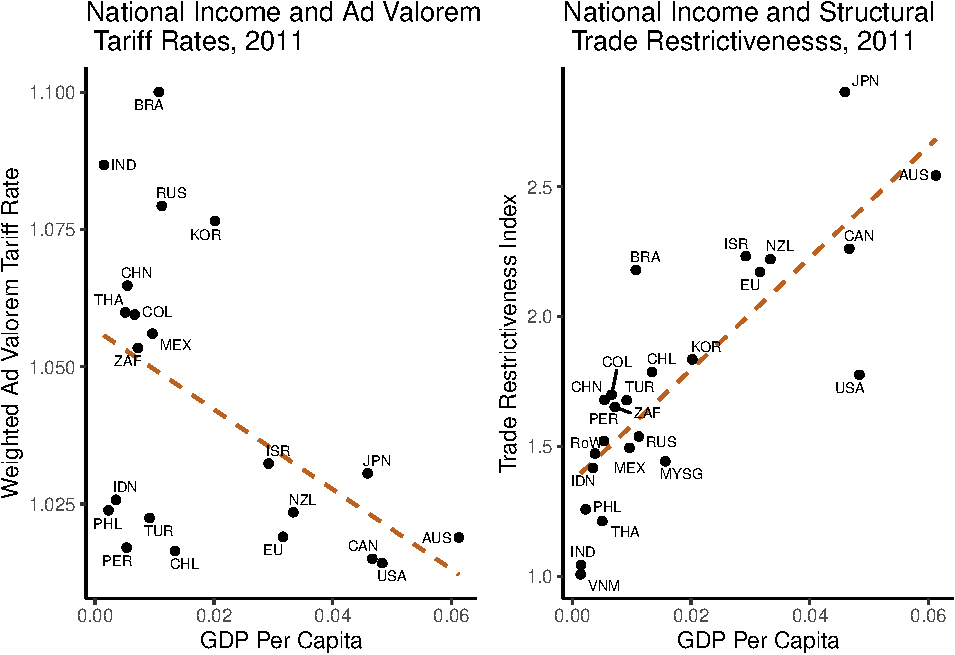
\includegraphics{figure/triIncome-1.pdf}
\caption{Tariff rates (left) and structural trade restrictiveness
(right) against GDP per capita \label{fig:triIncome}}
\end{figure}

The trade policy openness attributed to developed countries also depends
strongly on the metric used to evaluate openness.\footnote{See Rodríguez
  and Rodrik (2000), Dollar and Kraay (2004), and Tavares (2008) for
  discussions of this phenomenon.} As shown in Figure
\ref{fig:triIncome}, there is a negative association between economic
development (per capita GDP) and applied tariff rates. This relationship
is reversed if trade policy restrictiveness is measured as proposed
here. Countries with higher per capita incomes tend to have higher Trade
Restrictiveness Indices.\footnote{See Equation \ref{eq:tri}.} This is
consistent with Kono (2006) and Queralt (2015), which suggest that
developed countries offset tariff reductions with increases in
non-tariff direct barriers and (potentially distortionary) domestic
taxes.

This paper is most closely related to the international economics
literature on the estimation of trade costs, beginning with Anderson and
Van Wincoop (2004). The particular methodology adopted here draws on
several studies that link price gaps to these trade costs (Eaton and
Kortum 2002; Waugh 2010; Simonovska and Waugh 2014; Sposi 2015; Waugh
and Ravikumar 2016). I build on these studies by disentangling policy
barriers to trade and freight costs, and connecting the implied policy
barriers to observable trade policy instruments. A parallel literature
focuses on the estimation of trade costs under the assumption that they
are symmetric (Head and Ries 2001; Novy 2013).\footnote{Bergstrand,
  Egger, and Larch (2013) provide an alternative method to estimate the
  asymmetric barriers targeted here.} While transportation costs may be
nearly symmetric, policy barriers are less likely to be (Kono 2008;
Tavares 2008). Such estimates therefore average over meaningful policy
heterogeneity.

The paper is also related to efforts to use observable barriers to trade
to construct indices of trade openness (Sachs and Warner 1995; Anderson
and Neary 1996; Kee, Nicita, and Olarreaga 2009). These observable
barriers may be a non-random sample from the universe of protectionist
instruments, however. Here, I take advantage of the structure of the
theoretical model to infer the magnitude of policy barriers from the
price and trade data, rather than attempting to quantify observable
barriers. Hiscox and Kastner (2002) construct country-level measures of
aggregate trade openness using a fixed effects approach. Martini (2018)
constructs industry-level measures of trade restrictiveness, under the
assumption that policy barriers are nondiscriminatory within industry. I
sacrifice industry-level granularity in order to assess discrimination
in the international trade policy regime.

The fields of comparative and international political economy rely
heavily on imperfect measures of trade protectionism. Political economic
theories of protectionism generally relates primitives of the economic
and political environment to a government's choice of trade policy,
broadly construed. In evaluating these theories, however, researchers
generally resort to examining observable barriers to trade, such as
applied tariff rates, NTM coverage ratios, or simply the volume of
trade.\footnote{For a few examples, see Goldberg and Maggi (1999);
  Mansfield, Milner, and Rosendorff (2000); Milner and Kubota (2005);
  Tavares (2008); Kono (2009); Gawande, Krishna, and Olarreaga (2009);
  Betz (2017); Barari, Kim, and Wong (2019).} The measure constructed
here is arguably closer to the theoretical quantity of interest of many
of these studies.

The broad policy barriers recovered here are also the objects that
governments seek to influence in international negotiations,
particularly in today's era in which tariffs rates are historically
low.\footnote{For example, Trans Pacific Partnership (TPP) negotiations
  focused overwhelmingly on non-tariff liberalization efforts.
  Fergusson, Ian F. and Brock R. Williams.
  \href{https://fas.org/sgp/crs/row/R44489.pdf}{``The Trans-Pacific
  Partnership (TPP): Key Provisions and Issues for Congress.''} 14 June,
  2016. Congressional Research Service.} Governments desire foreign
market access for the firms whose interests they represent (Gawande,
Krishna, and Olarreaga 2009; Ossa 2011, 2012). Acquiring foreign market
access requires dismantling policy barriers to trade, direct and
indirect. This places governments in a complex multilateral bargaining
game that has attracted the attention of many studies.\footnote{See, for
  example, Hirschman (1945); Pollins (1989a); Gowa and Mansfield (1993);
  Milner (1997); Aghion, Antràs, and Helpman (2007); Head, Mayer, and
  Ries (2010); Antràs and Padró i Miquel (2011); Dube, Kaplan, and Naidu
  (2011); Berger et al. (2013); Ossa (2014).} Evaluating and assessing
the outcomes of this game requires measurement of its outcomes --
governments' trade policy choices.

Finally, many argue that international institutions, the WTO and its
predecessor General Agreements on Tariffs and Trade (GATT) in
particular, structure this bargaining game in important ways (Bagwell
and Staiger 1999; Maggi 1999; Steinberg 2002; Davis 2006; Carnegie 2014;
Bagwell, Staiger, and Yurukoglu 2018a). GATT signatories committed in
principle to convert protective policy measures into tariff-equivalents
and subsequently negotiated primarily over tariff barriers (Bagwell and
Staiger 2004). Theories of international trade institutions generally
take this commitment seriously, assuming commitments to reduce tariffs
cannot be subsequently ``undone'' through the implementation of
non-tariff or behind-the-border barriers to trade. Statements about the
efficacy of the principles of reciprocity and nondiscrimination in
achieving efficient outcomes rest on this premise.

I proceed in three steps. The next section specifies a model of
international trade and demonstrates how it relates observables to the
magnitude of trade policy distortions. I then discuss the data that I
use to calibrate the model. Finally, I present the results of this
exercise and discuss their implications for the question posed at the
beginning of this paper -- is international trade free and fair?

\section{Model}

In 2011, tradable goods were, on average, twice as expensive in Japan
than in Malaysia.\footnote{See The World Bank,
  \href{http://www.worldbank.org/en/programs/icp\#1}{International
  Comparison Program (ICP)}} If trade were frictionless, Malaysian
merchants could exploit this price difference by shipping goods to
Japan, making more than twice what they would be selling their goods in
their home market. Factually, however, Malaysian exporters made up less
than one percent of the market for tradables in Japan in 2011. The model
explicated below allows me to infer that these prospective exporters
must have faced high costs to sell in the Japanese market and to
quantify the exact magnitude of these costs. If freight costs are known,
then the component of these costs attributable to policy distortions can
be recovered separately.

Eaton and Kortum (2002) and Waugh (2010) show that these forces are
related in a simple equation. Let \(d_{ij} \geq 1\) denote the iceberg
cost of shipping goods from \(j\) to \(i\),\footnote{By the iceberg
  assumption, for every \(d_{ij}\) units shipped from \(j\) to \(i\), 1
  unit arrives. \(d_{ij} - 1\) is the ad valorem value of the aggregate
  tax firms in \(j\) face to export to \(i\).} \(\lambda_{ij}\) denote
\(j\)'s market share in \(i\), and \(P_i\) denote the aggregate price of
tradables in \(i\). Then, \begin{equation} \label{eq:Waugh}
d_{ij} = \left( \frac{\lambda_{ij}}{\lambda_{jj}} \right)^{-\frac{1}{\theta}} \frac{P_i}{P_j}
\end{equation} where \(\theta > 1\) is the trade elasticity.\footnote{Here,
  \(\lambda_{jj}\) is the share of \(j\)'s market for tradables that is
  captured by producers within \(j\).} If \(\theta\), price levels, and
market shares are known, then this equation can be used to measure trade
frictions exporters in \(j\) face when selling in market \(i\)
(\(d_{ij}\)). If aggregate prices are equal in both markets
(\(P_i=P_j\)), then \(j\)'s relative market penetration informs directly
about trade barriers. As \(\lambda_{ij}\) goes up, the implied barrier
\(d_{ij}\) goes down. When \(j\)'s share in \(i\)'s market is equivalent
to its share in its own market (\(\lambda_{ij}=\lambda_{jj})\), we infer
that \(j\) faces no barriers to export to \(i\)
(\(d_{ij}=1\)).\footnote{This is a natural result of the assumption of
  consumer homogeneity.} Now, assume that aggregate prices in \(i\) and
\(j\) differ. Specifically, let \(P_i > P_j\). In the absence of trade
costs, this would generate an arbitrage opportunity for
high-productivity producers in \(j\) -- they can profit by shipping
goods to \(i\) and taking advantage of higher prices. If trade were
frictionless, then we must have \((\lambda_{ij} > \lambda_{jj})\). The
extent to which this relationship holds in the data informs about the
magnitude of barriers to trade.

This relationship between cross national tradable prices, trade flows,
and trade costs follows from the competitive framework of Eaton and
Kortum (2002), adapted to the study of trade costs by Waugh (2010). In
the model presented below, I modify their underlying framework in order
to minimize the conceptual distance between the theory and the data.
However, the result is not unique to competitive international
economies. Quantitative trade models with market imperfections generate
related ``gravity'' equations that imply the same relationship between
prices, trade, and trade costs (Melitz 2003; Chaney 2008; Costinot and
Rodríguez-Clare 2015).

\subsection{Environment}

There are \(N\) countries in the international economy, indexed
\(i \in \left\{ 1, ..., N \right\}\). Within each country resides a
representative consumer, with labor endowment \(L_i\). The setup follows
closely Eaton and Kortum (2002), so I omit some derivations of the
quantities presented here and direct readers to their paper. To match
the data on consumer expenditure on tradable goods, I consider a variant
of their model which consumers value both tradable goods and nontradable
services. Then, gross consumption of tradables in the economy is simply
gross consumption (including final and intermediate goods) minus
consumer expenditure on services. This is the denominator I use in
calculating trade shares when calibrating the model.

\subsubsection{Consumption}

Each consumer values aggregate tradable goods \(Q_i\) and aggregate
nontradable services \(S_i\), which are combined in a Cobb-Douglas
utility function \begin{equation} \label{eq:CD}
U_i = Q_i^{\nu_i} S_i^{1 - \nu_i} .
\end{equation} A country-specific parameter \(\nu_i \in [0,1]\) governs
the consumer's relative preference for goods over services. Wages are
denoted \(w_i\), which implies country gross domestic products are given
by \[
I_i = w_i L_i .
\] Cobb-Douglas preferences imply consumers will spend a fraction
\(\nu_i\) of their income on tradable goods.\footnote{In calibrating the
  model, I choose \(\nu_i\) to match the factual expenditure shares on
  tradables in each country, as reported by the ICP.} Equilibrium
consumer expenditure on tradables is then \[
E_i^q = \nu_i I_i + D_i
\] where \(D_i\) is the value of exogenously given trade deficits.

There is a continuum of tradable varieties, indexed by
\(\omega \in [0, 1]\). There is a set \(\mathcal{K}\) of tradable good
categories indexed \(k \in \left\{ 0, ..., K - 1 \right\}\). Let \[
h : \Omega \rightarrow \mathcal{K}
\] be a function that associates varieties with good categories. The set
of goods in category \(k\) is \(\Omega_k\) where \[
\Omega_k = \left\{ \omega : h(\omega) = k \right\} .
\] The mass of each tradable good category is \(1 / K\).

Consumer utility over these varieties exhibits constant elasticity of
substitution (CES) \begin{equation} \label{eq:CES}
Q_i = \left( \int_{[0,1]} \tilde{\alpha}_{i, h(\omega)}^{\frac{1}{\sigma}} q_i(\omega)^{\frac{\sigma - 1}{\sigma}} d \omega \right)^{\frac{\sigma}{\sigma - 1}}
\end{equation} with \(\sigma > 0\).
\(\tilde{\alpha}_{ik} = \epsilon_{ik} \alpha_k\) is a stochastic
preference parameter that modulates country \(i\)'s consumer's relative
preference for goods in category \(i\). These preferences are constant
across consumers in different countries up to a shock,
\(\epsilon_{ik}\), with \(\E [ \epsilon_{ik} ] = 1\).

With expenditure on tradables fixed by the Cobb Douglas upper level
preference structure, consumers simply maximize \(Q_i\) subject to their
tradable budget constraint,
\(\int_{[0,1]} p_i(\omega) q_i(\omega) d \omega \leq E_i^q\), where
\(p_i(\omega)\) is the (endogenous) price of variety \(\omega\) in
country \(i\). The aggregate price of tradables in country \(i\) is as
in Dixit and Stiglitz (1977) \begin{equation} \label{eq:P}
P_i = \left( \int_{[0,1]} \tilde{\alpha}_{i, h(\omega)} p_i(\omega)^{1 - \sigma} d \omega \right)^{\frac{1}{1 - \sigma}} .
\end{equation}

\subsubsection{Production}

Every country can produce every tradable variety \(\omega\). Each
country has an underlying mean productivity level \(T_i\), but
\(\omega\)-specific productivities \(z_i(\omega)\) are modeled as the
realization of a random variable drawn from a Frechet distribution.
Production requires both labor and a composite intermediate good that is
exactly analogous to an aggregate consumption good \(Q_i\). The cost of
producing a unit of variety \(\omega\) is \begin{equation} \label{eq:c}
c_i(\omega) = \frac{1}{z_i(\omega)} w_i^{1 - \beta} P_i^{\beta}
\end{equation} where the global parameter \(\beta \in [0, 1]\) governs
the share of intermediates required in production.\footnote{Services are
  produced at cost \(c_i^s = \frac{w_i}{A_i}\), where \(A_i\) is a
  country-specific services productivity.} Let \(X_i\) denote the value
of tradable production in country \(i\). A constant share, \(\beta\), of
this value will be spent on intermediates \[
E_i^x = \beta X_i .
\]

Countries require \(1/z_i(\omega)\) labor-intermediate bundles to
produce one unit of variety \(\omega\). Markets are competitive, so
prices are equal to marginal costs. The local price (\(p_{ii}(\omega)\))
of variety \(\omega\) is therefore \begin{equation} \label{eq:pii}
p_{ii}(\omega) = c_i(\omega) .
\end{equation}

\(\omega\)-specific productivities are stochastic. Let \(F_i(z)\) denote
the probability that country \(i\)'s productivity is less than or equal
to \(z\), formally \[
F_i(z) = \text{Pr} \left( z_i(\omega) \leq z \right) .
\] When \(F_i(z)\) is distributed Frechet,
\begin{equation} \label{eq:Frechet}
F_i(z) = \exp \left( - T_i z^{-\theta} \right) .
\end{equation} The country-wide technology level \(T_i\) shifts country
\(i\)'s productivity distribution -- higher values of \(T_i\) imply
higher productivity values on average. \(\theta > 1\) is a global
parameter that governs the variance of the productivity
draws.\footnote{In equilibrium, it serves as the elasticity of trade
  flows to trade costs. As producers become more heterogeneous, trade
  becomes more sensitive to changes in costs.}

Exporters pay iceberg costs (\(d_{ji} \geq 1\)) to ship goods abroad.
The price in country \(j\) of varieties produced in \(i\) is therefore
\[
p_{ji}(\omega) = d_{ji} p_{ii}(\omega) .
\] These costs are affected by transportation infrastructure at home and
abroad, international freight costs, and policy distortions. Below, I
present a framework for disentangling these costs and isolating the
magnitude of distortions attributable to policy.

Domestic consumers and producers alike search around the world for the
cheapest source of each variety \(\omega\). The equilibrium price of
variety \(\omega\) in country \(i\) must satisfy \[
p_i^\star(\omega) = \min_{j \in \left\{ 1,...,N \right\}} \left\{ p_{ij} \right\} .
\]

\subsection{Equilibrium}

For national accounts to balance, gross output and gross consumption,
inclusive of trade deficits \(D_i\), must be equal.
\begin{equation} \label{eq:accounts}
I_i + \beta X_i + D_i = E_i^q + E_i^x + (1 - \nu_i) I_i
\end{equation} Total income is given by the sum of domestic payments for
services and labor payments from the global sales of tradables, \(X_i\),
or \[
I_i = w_i L_i = (1 - \beta) X_i + (1 - \nu_i) I_i .
\] Substituting into Equation \ref{eq:accounts} requires
\begin{equation} \label{eq:tIncome}
X_i = E_i^q + E_i^x - D_i
\end{equation} or that trade less deficits is balanced.

Total expenditure on tradables is the sum of expenditures from consumers
and producers\footnote{Note that expenditure on tradables can be written
  \[E_i = I_i + \beta X_i + D_i - (1 - \nu_i) I_i \] or gross
  consumption less consumer expenditure on services. This is the
  empirical quantity for \(E_i\) I use when calibrating the model.} \[
E_i = E_i^q + E_i^x .
\] Let \(\lambda_{ij}(\bm{w})\) denote the share of expenditure on
tradables country \(i\) spends on goods from \(j\) and \[
\Omega_{ij}^\star = \left\{ \omega \in [0,1] \left. \right\vert p_{ij}(\omega) \leq \min_{k \neq j} \left\{ p_{ik} \right\} \right\} .
\] Then \begin{equation} \label{eq:lambda}
\lambda_{ij}(\bm{w}) = \frac{1}{E_i} \int_{\Omega_{ij}^\star} p_{ij}(\omega) q_i \left( p_{ij} (\omega) \right) d \omega
\end{equation} where \(q_i \left( p_{ij} (\omega) \right)\) is
equilibrium consumption of variety \(\omega\) from both producers
(intermediates) and consumers (final goods).

This quantity depends on wages everywhere, stored in the vector
\(\bm{w} = \left\{ w_1, ..., w_N \right\}\). Note that given exogenous
labor endowments \((L_i)\), trade costs \((d_{ij})\), technologies
\((T_i)\), and parameters
\(\left\{ \sigma, \theta, \nu_i, \beta \right\}\), endogenous wages
completely determine the pattern of trade. Gross income in country \(i\)
from the sale of tradables can be written
\begin{equation} \label{eq:marketClearing}
X_i = \sum_{j=1}^N \lambda_{ji}(\bm{w}) E_j .
\end{equation}

\textbf{Definition:} An \emph{international equilibrium} is a vector of
wages \(\bm{w}\) such that Equations \ref{eq:tIncome}, \ref{eq:lambda},
and \ref{eq:marketClearing} hold for all
\(i \in \left\{1, ..., N \right\}\).

Alvarez and Lucas (2007) provide an argument for the existence and
uniqueness of such an equilibrium. In the unique equilibrium, trade
shares satisfy \begin{equation} \label{eq:Gravity}
\lambda_{ij}(\bm{w}) = \frac{ T_j \left( d_{ij} w_j^{1 - \beta} P_j^{\beta} \right)^{- \theta} }{\Phi_i}
\end{equation} where \[
\Phi_i =  \sum_j T_j \left( d_{ij} w_j^{1 - \beta} P_j^{\beta} \right)^{- \theta} .
\] The equilibrium price index in country \(i\) is
\begin{equation} \label{eq:eqP}
P_i = \gamma \Phi_i^{ - \frac{1}{\theta} }
\end{equation} where \(\gamma\) is a function of exogenous
parameters.\footnote{Specifically,
  \[\gamma = \Gamma \left( \frac{\theta + 1 - \sigma}{\theta} \right)^{ \frac{1}{1 - \sigma} }\]
  and \(\Gamma\) is the gamma function.}

The numerator of Equation \ref{eq:Gravity} is a measure of the overall
competitiveness of country \(j\). Naturally, increasing average
productivity increases \(j\)'s market penetration everywhere. Decreasing
wages in \(j\) has the same effect. Decreasing trade costs between \(i\)
and \(j\) \((d_{ij})\) also increases \(\lambda_{ij}\). The denominator
is a ``multilateral resistance'' (Anderson and Van Wincoop 2003) term
that captures the overall level of competitiveness in country \(i\). All
else equal, it is easier to penetrate the market in country \(i\) if
others struggle to penetrate it, due to inferior technology, high wages,
and/or high bilateral trade costs.

\subsection{Isolating Policy Barriers}

To get from the factory gates of a firm located in an exporting country
and the market located overseas, goods incur a bevy of costs, both
economic and political in nature. Our goal is to recover the proportion
of these costs attributable to \emph{policy} barriers to trade. I assume
that trade costs are multiplicatively decomposable into
exporter-specific costs,\footnote{This includes both costs associated
  with transportation within the exporting country and any taxes and
  regulatory costs that are common to all traders in the country (Limao
  and Venables (2001)).} international freight costs, and policy
barriers to trade. Note that I do not model heterogeneity in costs
common to all traders within \emph{importing} countries. This framework
yields \begin{equation} \label{eq:tcosts}
d_{ij} = \rho_j \delta_{ij}(\bm{Z}_{ij}) \tau_{ij}
\end{equation} where \(\rho_j\) denotes exporter-specific costs,
\(\delta_{ij}\) denotes international freight costs, and \(\tau_{ij}\)
denotes policy barriers. \(\delta_{ij}\) is a function, which takes a
vector of bilateral geographic covariates \(\bm{Z}_{ij}\) and outputs
bilateral freight costs.\footnote{I discuss how I model these costs in
  more detail in Appendix B.} I normalize
\(\delta_{ii} = \tau_{ii} = 1\).

\begin{figure}
\centering
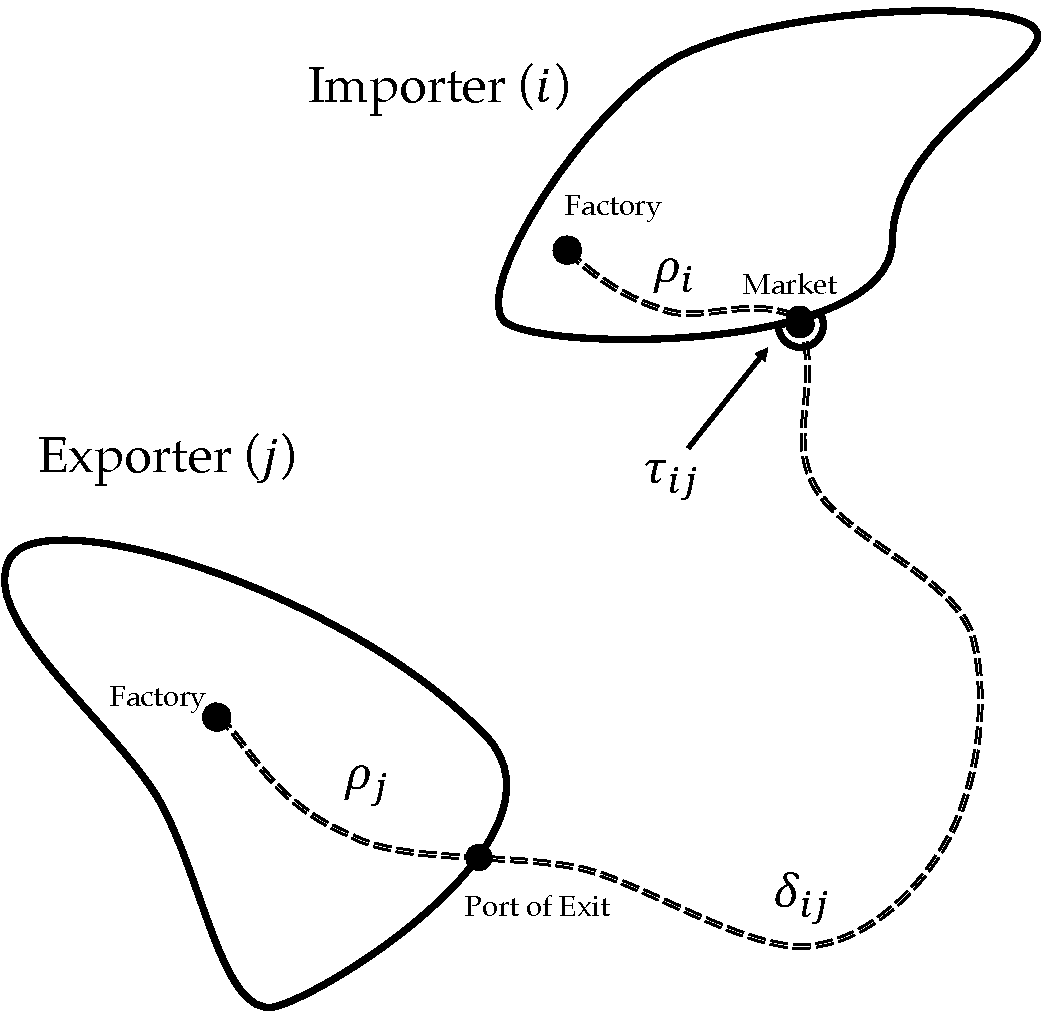
\includegraphics[width=4in,height=4in]{figure/tcosts.pdf}
\caption{Trade cost decomposition. \label{fig:tcostsMap}}
\end{figure}

Figure \ref{fig:tcostsMap} traces the path goods must travel from a
factory in country \(j\) to a market in country \(i\). Goods first
travel from the factory in \(j\) to \(j\)'s border. Upon reaching the
border (airport, port, or border crossing), goods must travel by land,
sea, or air to the border of their destination country. Along the way,
they incur freight costs \(\delta_{ij}\). The market in \(i\) is
protected by a policy barrier \(\tau_{ij}\) that can vary across
importers. Once goods cross this border, they arrive at the market and
are consumed at a price inclusive of the factory gate price
\(p_{jj}(\omega)\) and these transportation and policy costs.
Substituting Equation \ref{eq:tcosts} into the gravity equation
\ref{eq:Gravity} gives \[
\lambda_{ij} = \frac{ T_j \left( \rho_j \delta_{ij}(\bm{Z}_{ij}) \tau_{ij} w_j^{1 - \beta} P_j^{\beta} \right)^{- \theta} }{\Phi_i} .
\]

The problem with taking this equation straight to the data is that it
contains unobserved technologies and wages. This would also require
taking a stance on several structural parameters. Comparing \(j\)'s
import penetration in \(i\) to its share of the home market
\(\lambda_{jj}\) solves this problem, however. To see this, note \[
\frac{\lambda_{ij}}{\lambda_{jj}} = \left( \delta_{ij}(\bm{Z}_{ij}) \tau_{ij} \right)^{- \theta} \frac{\Phi_j}{\Phi_i} .
\] Rearranging and substituting from Equation \ref{eq:eqP} gives the
familiar relationship in Equation \ref{eq:Waugh} discussed above,
modified to separate trade barriers from freight costs:\footnote{Note
  that given prices, freight costs, and \(\lambda_{jj}\), trade flows
  are a ``sufficient statistic'' for the magnitude of policy barriers to
  trade. In the face of opaque policy instruments, this provides a
  rationale for simply demanding bilateral trade deficit reductions in
  trade negotiations, a tactic utilized by the Trump administration in
  negotiations with China. Wei, Lingling.
  \href{https://www.wsj.com/articles/u-s-wants-200-billion-cut-in-china-trade-imbalance-by-end-of-2020-1525419253}{``U.S.
  and China Make Scant Progress in Trade Talks.''} \emph{The Wall Street
  Journal}. 4 May, 2018.} \begin{equation} \label{eq:tau}
\tau_{ij} = \left( \frac{\lambda_{ij}}{\lambda_{jj}} \right)^{-\frac{1}{\theta}} \frac{P_i}{P_j} \frac{1}{\delta_{ij}(\bm{Z}_{ij})} .
\end{equation}

If the trade elasticity is known, data on trade shares, relative prices,
and freight costs are sufficient to calculate policy barriers to trade,
\(\tau_{ij}\). In the next section, I discuss how these data are
constructed to match the model presented here.

\section{Calibration and Estimation}

I present results from a calibration on a set of 24 of the world's
largest economies in 2011.\footnote{The list of the economies in the
  sample is included in Appendix E.} These in-sample countries
collectively made up 87 percent of world GDP. I treat the rest of the
world as an aggregate outside economy. The calibration requires me to
take a stance on a single structural parameter, the Frechét parameter,
\(\theta\). I set \(\theta =\) 6, in line with the estimates from the
structural gravity literature (Head and Mayer 2014).

Price indices and freight costs estimated below are measured with error.
I employ a nonparametric bootstrap to quantify the uncertainty
surrounding the implied magnitude of policy barriers. This entails
sampling product-level prices and observed freight costs with
replacement and recomputing \(\tau_{ij}\) many times.

\subsection{Prices and Consumer Expenditures}

In order to calculate policy barriers to trade, I require an empirical
analogue of the Equation \ref{eq:P}, the country-specific price index.
This quantity summarizes the overall level of competition in the
economy, summarized in the market price of tradable varieties. Data on
cross-national prices comes from the World Bank's International
Comparison Program, used to calculate Purchasing Power Parities
(PPP).\footnote{Rao (2013) details the underlying data and methodology.
  Deaton and Heston (2010) discusses challenges in working with these
  data.}

The ICP surveys prices of hundreds of products and services across 146
countries, and chooses product lists to maximize comparability across
markets. They also report the share of GDP that is allocated toward
purchases of different product categories, termed ``basic headings.''
After using the prevailing exchange rate to convert prices into U.S.
dollars, various (largely atheoretical) statistical methods are used to
compute internationally comparable price indices across basic
headings.\footnote{See Redding and Weinstein (2018) for a discussion of
  the conditions under which these price indices correspond to their
  theoretical counterparts.} I classify each basic heading as tradable
or nontradable and report the results of this classification in Appendix
F.\footnote{Simonovska and Waugh (2014) undertake the same exercise. My
  classification differs slightly from theirs.}

I take these basic headings as the empirical analogue to good categories
\(k\) in the model. I assume that the local price of each variety in
category \(k\) is constant,
\(p_i(\omega) = p_i(\omega^\prime) = p_{ik}\) for all
\(\omega, \omega^\prime \in \Omega_k\). Then, the price index in
Equation \ref{eq:P} can be written \[
P_i = \left( \int_\omega \tilde{\alpha}_{i, h(\omega)} p_i(\omega)^{1 - \sigma} \right)^{\frac{1}{1 - \sigma}} = \frac{1}{K} \left( \sum_k \tilde{\alpha}_{ik} p_{ik}^{1 - \sigma} \right)^{\frac{1}{1 - \sigma}} .
\] The ICP reports prices relative to their levels in the United States.
In Appendix A, I show consumers' demand for each good is a function
their preferences (\(\tilde{\alpha}_{ik}\)), the good's price
(\(p_{ik}\)), and the price level in the country (\(P_i\)). Differencing
this demand equation with respect to its analogue in the United States
eliminates the constant portion of the preference parameter,
\(\alpha_k\). Then, demand relative to the United States is a function
of the stochastic preference shocks (\(\epsilon_{ik}\)), the price of
the good, and the overall price level in the country. I estimate this
differenced equation on observed prices and relative expenditure shares
by minimizing the squared magnitudes of the preference shocks. This
generates estimates for the country-specific price indices,
\(\hat{P}_i\).

\begin{figure}
\centering
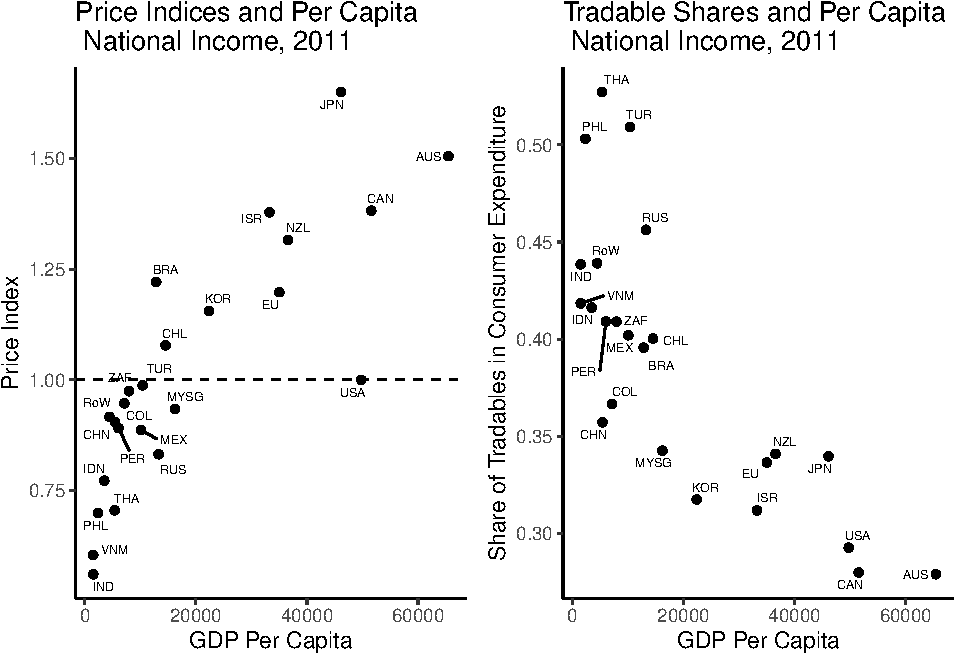
\includegraphics{figure/P-1.pdf}
\caption{Price index estimates and tradable expenditure shares
\label{fig:P}}
\end{figure}

I plot the distribution of estimated price indices and tradable
expenditure shares on tradables that emerge from this procedure against
per capita GDPs in Figure \ref{fig:P}. Within my sample, consumers in
wealthier countries tend to face higher prices. The total share of
consumer expenditure on tradable goods \((\sum_{k=0}^{K-1} x_{ik})\) is
the empirical analogue to \(\nu_i\). On average, consumers spend 40
percent of their income on tradable goods.

\subsection{Expenditure Shares}

The theory makes predictions about the share of consumer expenditure
that will be devoted to products from each country. In the data,
however, I only observe the value of imports \emph{at the border}. Price
distortions due to policy barriers to trade are not included in the
valuations of shipments. Let \(\lambda_{ij}^{\text{cif}}\) denote the
share of \(i\)'s expenditure on tradables spent on goods from \(j\),
inclusive of freight rates and exclusive of policy barriers.\footnote{While
  tariffs are usually assessed on the f.o.b. value of shipments,
  non-tariff barriers cannot be tailored in this manner. For this
  reason, I assume the costs of policy barriers are assessed on
  shipments' c.i.f. values.} We can then write
\(\lambda_{ij} = \tau_{ij} \lambda_{ij}^{\text{cif}}\) and
\begin{equation} \label{eq:lambda_jj}
\lambda_{jj}(\bm{\tau}_j) = \left( 1 - \sum_{i \neq j} \tau_{ji} \lambda_{ji}^{\text{cif}} \right) .
\end{equation} This formulation requires that policy barriers to trade
are assessed ``behind the border,'' as discussed in the introduction.

Substituting this relationship into \ref{eq:tau} gives a modified
equation relating observed trade flows, prices, and freight rates to
unobserved policy barriers to trade \begin{equation} \label{eq:tauCIF}
\tau_{ij} = \left( \frac{\lambda_{ij}^{\text{cif}}}{\lambda_{jj}(\bm{\tau}_j)} \right)^{-\frac{1}{\theta + 1}} \left( \frac{P_i}{P_j} \right)^{\frac{\theta}{\theta+1}} \left( \frac{1}{\delta_{ij}(\bm{Z}_{ij})} \right)^{\frac{\theta}{\theta+1}} .
\end{equation}

Then, to calculate \(\lambda_{ij}^{\text{cif}}\) and \(\lambda_{jj}\), I
need data on international trade flows as well as the market share of
domestic tradables producers in their home market. Data on trade flows
comes from the United Nations'
\href{https://comtrade.un.org/db/default.aspx}{COMTRADE}, cleaned and
harmonized by \href{http://www.cepii.fr/CEPII/en/welcome.asp}{CEPII}'s
\href{http://www.cepii.fr/cepii/en/bdd_modele/presentation.asp?id=1}{BACI}.
BACI denominates trade flows in free on board (f.o.b. or pre-shipment)
value, so predicted cost, insurance, and freight (c.i.f. or
post-shipment) values can be calculated simply by multiplying these
flows by \(\delta_{ij}\), estimated below. Total domestic consumption on
tradables can then be inferred from national accounts data, which report
gross output, gross consumption, and GDP.\footnote{Gross consumption
  includes consumer final expenditure as well as producers' expenditure
  on intermediates and is inclusive of trade deficits.} I simply
subtract the share of consumer expenditure on services implied by the
ICP data from each country's gross consumption, which provides a measure
of gross consumption on tradables, the empirical analogue to
\(E_i = \nu_i I_i\). These national accounts data are taken from the
\href{http://www.wiod.org/home}{World Input Output Database (WIOD)}
(Timmer et al. 2015) and the
\href{https://stats.oecd.org/Index.aspx?DataSetCode=IOTS}{OECD's
National Input Output Tables}.

Note that implicit domestic consumption in Equation \ref{eq:lambda_jj}
depends on the magnitude of policy barriers to trade. This is because
consumers' expenditure on foreign goods inclusive of policy barriers is
greater than the value of these purchases observed at the border.
Because \(\lambda_{jj}(\bm{\tau}_j)\) is a decreasing function, a unique
solution to Equation \ref{eq:tauCIF} is guaranteed to exist, so I simply
iterate on the values of \(\bm{\tau}\) and \(\bm{\lambda}\) until
convergence.

\subsection{Freight Costs}

Freight costs are observed for only a subset of my sample. As depicted
in Figure \ref{fig:tcosts}, all freight costs I observe cover the cost
of shipments from border-to-border. They do not include costs that are
incurred during intranational transit (\(\rho_i\)), which are
differenced out of Equation \ref{eq:tau}.

I build a simple model of the transportation sector in order to estimate
freight costs out of sample, using data on observed freight costs and
modes of transportation along with geographic covariates. I assume there
is a competitive transportation sector in each mode (generating constant
freight costs) and that the costs of transportation within a mode depend
on dyadic geography. Observing these costs, a continuum of exporters in
each country-sector choose the mode with which to ship their products to
market abroad. Exporter-specific shocks lead to utilization of all modes
by some exporters. This model generates a simple multinomial logistic
functional form for predicted mode shares (Mcfadden 1974), which can be
estimated given data on predicted freight costs. Predicted freight costs
and mode shares can be aggregated to predict total trade costs, which
serve as the \(\delta_{ij}\) in Equation \ref{eq:tau}. This model, and
the data used to estimate it, are discussed in more detail in Appendices
B and C, respectively.

There are two limitations of this simple model of the transportation
sector. First, Takahashi (2011), Behrens and Picard (2011), and
Brancaccio, Kalouptsidi, and Papageorgiou (2020) show that there are
significant scale economies in international shipping. This contradicts
the assumption of elastic supply of transportation services. Moreover,
non-freight trade costs may affect the attractiveness of different ports
and the prices demanded by transportation services providers. For
example, Brancaccio, Kalouptsidi, and Papageorgiou (2020) show that the
level of tariffs applied on a countries \emph{exports} affect its
desirability as a shipping destination, affecting the price of freight
to that country. This implies that \(\delta_{ij}\) depends on
\(\tau_{ij}\), a feature my framework is unable to capture.\footnote{These
  features also rationalize asymmetric freight costs. Because the
  bilateral covariates used to estimate my model are symmetric between
  any two countries, predicted freight costs are nearly symmetric as
  well (\(\delta_{ij} \approx \delta_{ji}\)). Differences in the
  product-level makeup of trade are the only asymmetry introduced in my
  framework.}

Accounting for these features of the market for transportation services
would add considerable complexity to the framework developed here.
Moreover, the simple model I consider produces reasonable out-of-sample
fit, and estimated freight costs are small relative to estimated policy
barriers. Figure \ref{fig:freight} depicts factual and predicted freight
costs for the United States, Australia, New Zealand, and Chile in 2011.
The observations for New Zealand and Chile are out of sample -- the
model was not trained on these data.\footnote{The model of aggregate
  freight costs relies on information on transportation mode shares,
  which were not available for these countries. They do report
  c.i.f.-f.o.b. ratios, however.} Chile and New Zealand's predicted
bilateral freight costs have a mean absolute error of 2 percentage
points. Overall, predicted freight costs average 7 percent the value of
shipments and are positively correlated with distance.

\begin{figure}
\centering
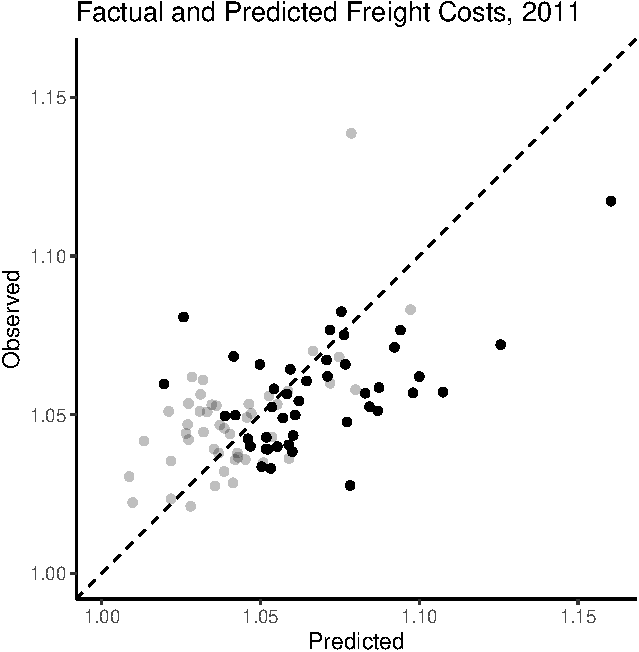
\includegraphics{figure/freight-1.pdf}
\caption{Factual versus predicted freight costs. In-sample observations
are shown in grey. Out-of-sample observations are shown in black.
\label{fig:freight}}
\end{figure}

\section{Results}

The results of this exercise reveal substantial unobserved policy
barriers to trade. In 2011, across all in-sample markets, exporters
faced an average \(\tau\) of 2.4, equivalent to a 140 percent import
tariff.\footnote{Of course, this result is sensitive to my stance on the
  trade elasticity. Doubling the trade elasticity to 12 cuts the average
  \(\tau\) to 1.62} The magnitude of these barriers dwarfs that of
applied aggregate tariffs, which average only 4 percent within my
sample. This result is consistent with Anderson and Van Wincoop (2003),
Bradford (2003), De Sousa, Mayer, and Zignago (2012), and Waugh and
Ravikumar (2016) which also uncover large implied trade costs using
indirect measurement methods. Figure \ref{fig:tcosts} shows the
distribution of implied policy barriers (panel A), relative to tariffs
and predicted freight costs.

\begin{figure}
\centering
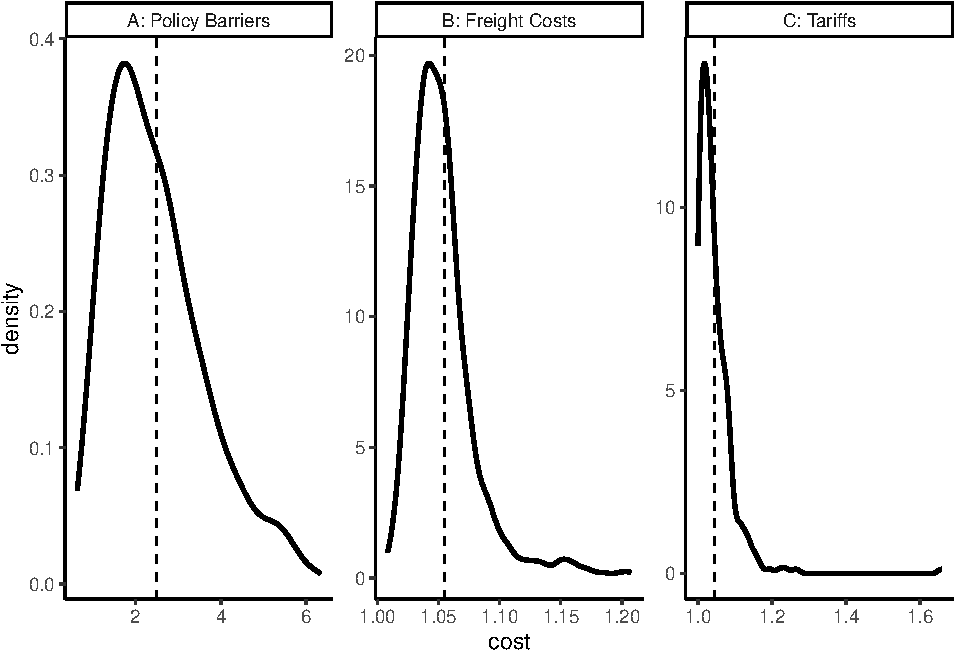
\includegraphics{figure/tcosts-1.pdf}
\caption{Distribution of freight costs, tariff barriers, and structural
policy barriers to trade (\(\tau_{ij}\)). Dashed lines show the mean of
each distribution. \label{fig:tcosts}}
\end{figure}

The model and data jointly suggest that international trade remains far
from free, even taking into account unavoidable freight costs. Returning
to Equation \ref{eq:tau}, this result suggests that the observed
international price gaps and trade flows are inconsistent with a trade
barrier-less world, given predicted freight costs. The model suggests
that if implied policy barriers were removed, some combination of
increases in trade flows and the reduction of price gaps would occur.

International trade is also far from fair. A fair international trading
system might allow for trade restrictions, but require that these
restrictions affect all trading partners equally. In fact, policy
barriers to trade are quite discriminatory. In 2011, the mean
within-country standard deviation of \(\tau_{ij}\) is 0.86, representing
a significant preferential margin for preferred trade partners. For
example, in 2011, U.S. trade with Canada (\(\tau_{ij} =\) 1.19), Japan
(1.21), and the European Union (1.4) was relatively unhindered.
Conversely, U.S. trade with Peru (3.11) and Vietnam (3.6) was highly
restricted.

\begin{figure}
\centering
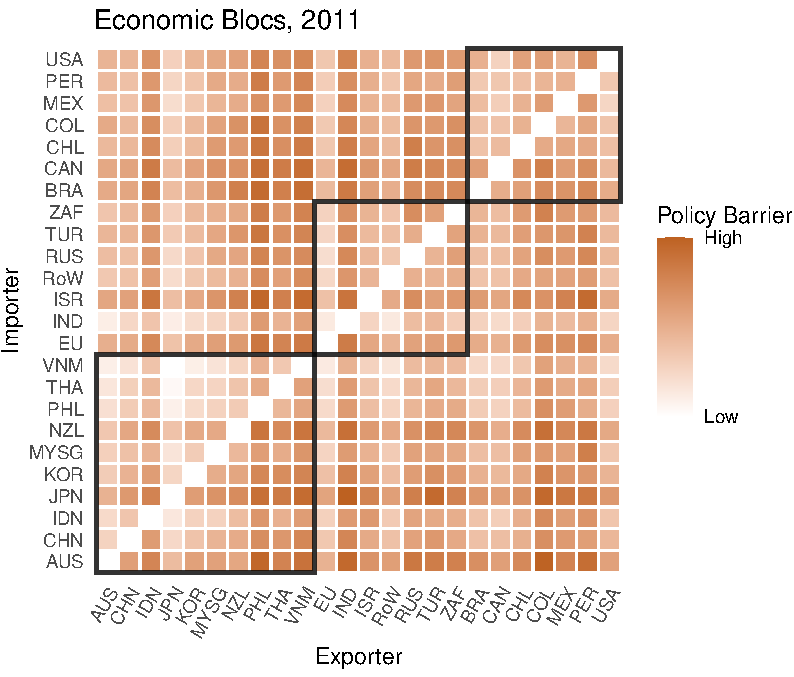
\includegraphics{figure/hm-1.pdf}
\caption{Distribution of policy barriers to trade. Each cell reports the
magnitude of the policy barrier each importing country (y-axis) imposes
on every exporting country (x-axis). Countries are partitioned into 3
groups through K-means clustering. Black rectangles enclose each
cluster. An interactive version of this plot is available at
\protect\url{https://brendancooley.shinyapps.io/epbt}. \label{fig:hm}}
\end{figure}

Figure \ref{fig:hm} shows the distribution of directed policy barriers
to trade in the data. The latent trade discrimination implemented by the
United States is not unique -- openness varies significantly at the
importer-exporter level. Clustering countries by the similarity of their
trade policy vectors uncovers regional biases in trade policy. I sort
countries into economic blocs through a K-means procedure with 3 groups.
Pacific countries (East and Southeast Asia and Australasia) are grouped
together, as are North and South American countries. The European Union
is grouped with Russia and Turkey. Because freight costs are not
included in these measures, these economic blocs are not the result of
mere geographic proximity. Rather, these countries have undergone
political-economic union by reducing policy barriers to trade on one
anothers' products.

Figure \ref{fig:tau_ci} plots uncertainty intervals surrounding the
magnitude of policy barriers for each importing country in the sample.
These intervals are asymmetric around the point estimates due to
nonlinearities in the estimating equation (\ref{eq:tau}).

\begin{figure}
\centering
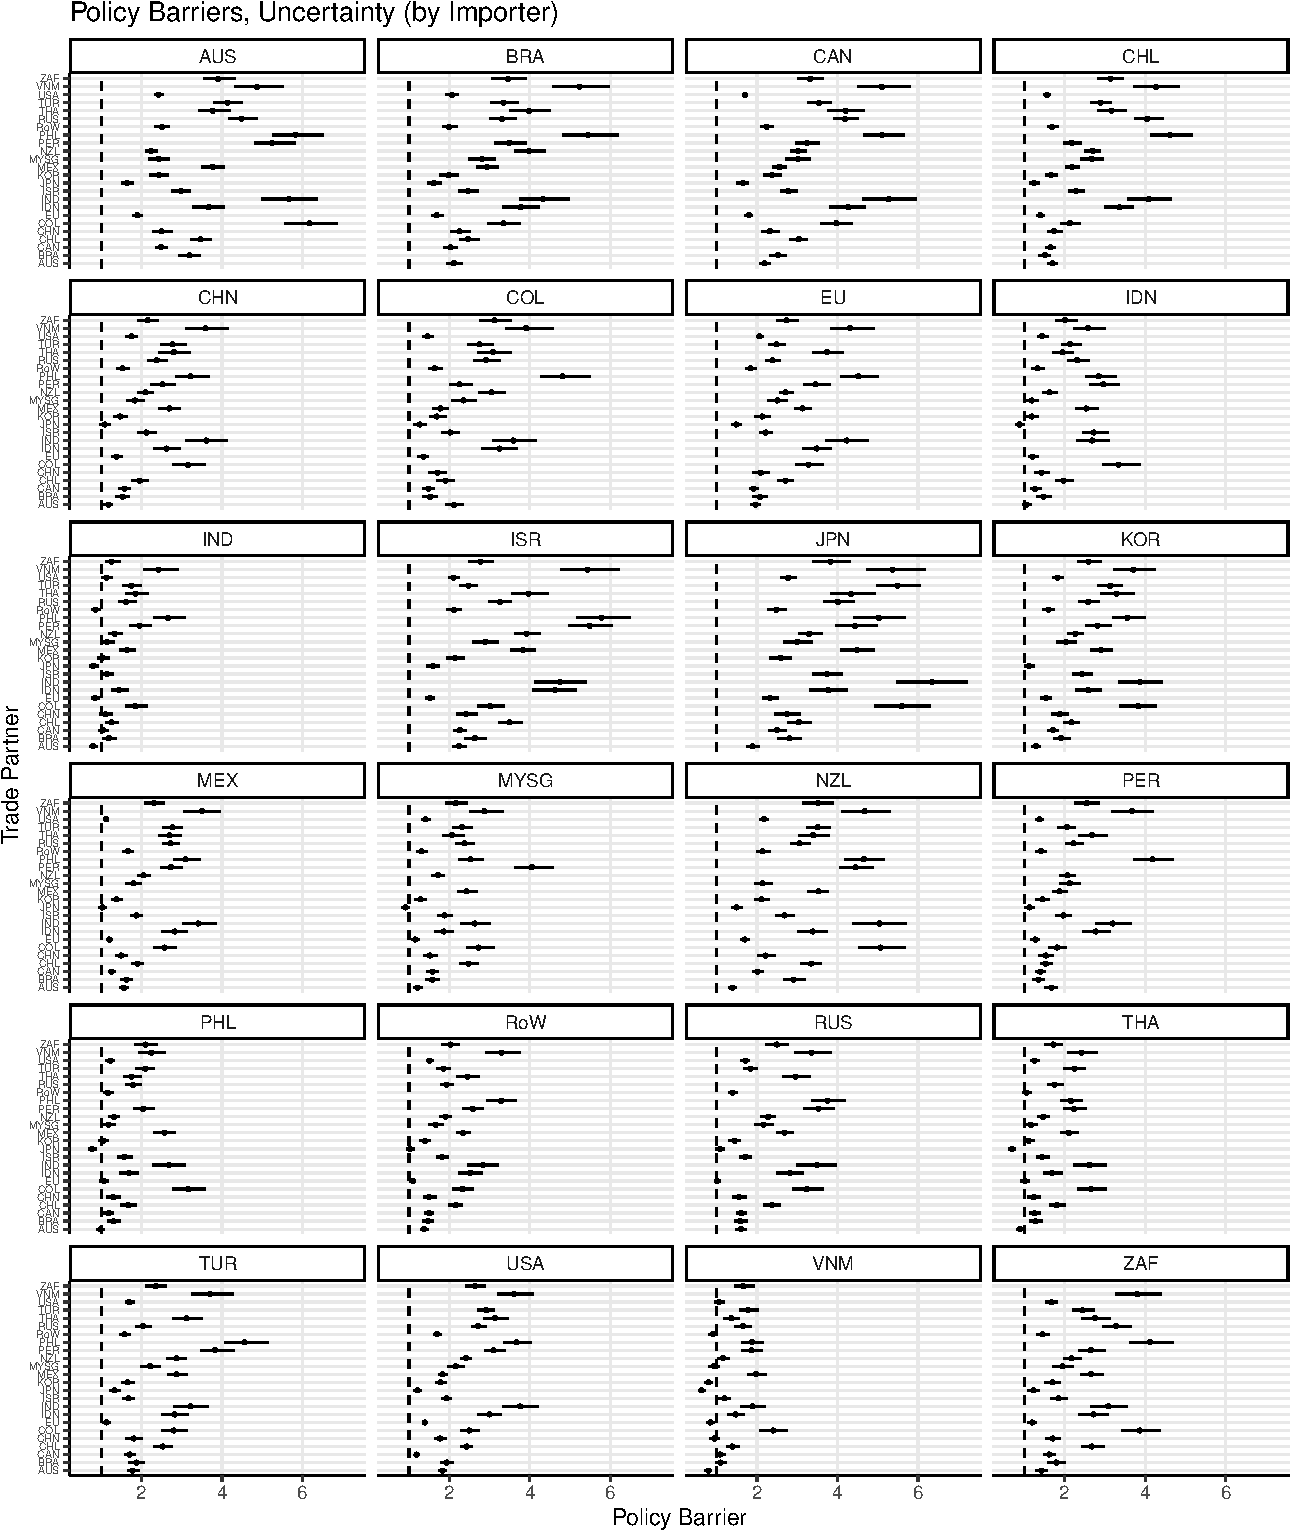
\includegraphics[width=6in,height=8in]{figure/tauq_ci.pdf}
\caption{Policy barrier estimates, magnitudes and uncertainty intervals.
Each panel displays the estimated policy barriers applied by an
importing country on products from every in-sample source country. An
interactive version of this plot is available at
\protect\url{https://brendancooley.shinyapps.io/epbt}.
\label{fig:tau_ci}}
\end{figure}

These barriers can be aggregated into two numbers -- a Trade
Restrictiveness Index (TRI) and a Market Access Index (MAI) -- that
summarize each country's import restrictiveness and international market
access conditions, respectively. The TRI is simply a weighted average of
the policy barriers an importing country imposes on all other countries,
where the weights are the gross tradable expenditures of these other
countries.\footnote{I use gross consumption, rather than observed flows,
  as weights for consistency with the theoretical framework. Trade flows
  are endogenous to each country's trade policy decisions. In a
  friction-less world, exporters would capture a constant share of every
  market's gross expenditure on tradables.}
\begin{equation} \label{eq:tri}
\text{TRI}_i = \frac{1}{\sum_{j \neq i} E_j} \sum_{j \neq i} \tau_{ij} E_j
\end{equation} Similarly, the market access index is an expenditure
weighted average of the barriers that all importing countries impose on
the exports of a given country. \begin{equation} \label{eq:mai}
\text{MAI}_j = \frac{1}{\sum_{i \neq j} E_i} \sum_{i \neq j} \tau_{ij} E_i
\end{equation} Higher values of the TRI correspond to higher aggregate
trade restrictiveness. Conversely, higher values of the MAI correspond
to lower aggregate market access (a high tax on a country's exports).

\begin{figure}
\centering
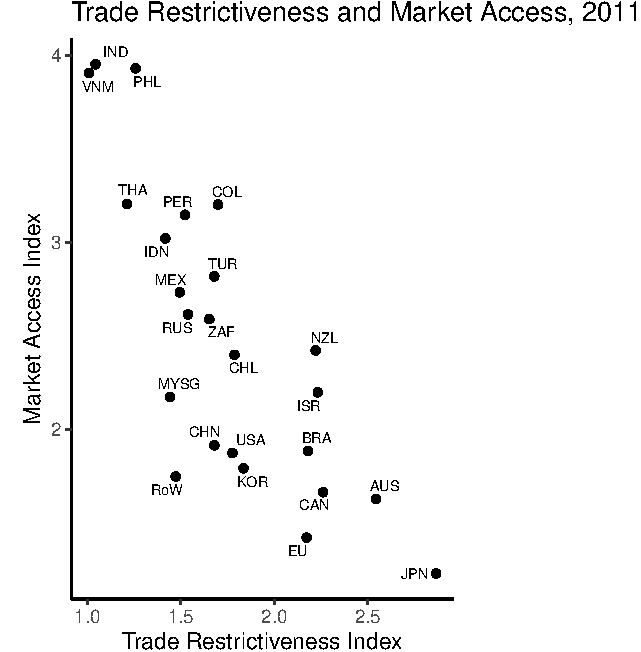
\includegraphics{figure/trimai-1.pdf}
\caption{Trade restrictiveness and market access conditions by country
\label{fig:trimai}}
\end{figure}

Figure \ref{fig:trimai} plots the TRIs and MAIs jointly. A negative
correlation between these indices emerges naturally from the structure
of the model. High domestic prices imply arbitrage opportunities,
raising the TRI. They also imply high opportunity costs for domestic
exporting firms that forgo these high prices. To rationalize these
flows, the model infers that these firms must face relatively friendly
market access conditions abroad, raising the MAI.

\subsection{Correlates of Unobserved Policy Barriers to Trade}

Figure \ref{fig:tcosts} shows that tariffs cannot account for the
magnitude of trade protection implied by the model. What, then, is the
source of these policy distortions? As discussed in the introduction,
governments have a dizzying slate of policy instruments at their
disposal which can have direct or indirect effects on trade. Existing
studies of trade protection generally leverage these observable proxies
of the broader, unobservable, aggregate policy barrier that is the
target of this study (Kee, Nicita, and Olarreaga 2009).

Such observable proxies include tariffs, but also NTMs and preferential
trade agreements (PTAs). NTMs are simply regulations that affect what
kinds of products can and cannot be imported. Some NTMs, such as quotas,
are rather blunt in their impact, while others, such as health and
safety regulations, are more subtle. PTAs usually lower tariff rates
beyond WTO commitments within a bloc of signatory countries.
Increasingly, these agreements also work to harmonize regulatory
environments and reduce ``behind-the-border'' barriers to trade (Baccini
2019). If in fact NTMs impede trade and PTAs facilitate trade, they
should be correlated with the aggregate policy barriers to trade
captured here.

To evaluate this proposition, I gather data on applied tariff rates,
NTMs, and PTAs, and run a simple regression to evaluate the correlation
between these observable indicators of trade restrictiveness and my
metric.

I measure aggregate tariff protection with a trade-weighted average of
applied tariff rates, taken from UN Conference on Trade and
Development's (UNCTAD)
\href{https://databank.worldbank.org/data/reports.aspx?source=UNCTAD-~-Trade-Analysis-Information-System-\%28TRAINS\%29\#}{TRAINS
database}.\footnote{This allows the measure to vary at the trade partner
  level, as exporters with different product portfolios are
  differentially exposed to tariff lines.} UNCTAD also tracks the
incidence of NTMs in governments official trade regulations. As is
standard in the literature on NTMs,\footnote{See, for example, Anderson
  and Van Wincoop (2004).} I employ NTM coverage ratios as a measure of
aggregate NTM protection. A coverage ratio is simply the proportion of
Harmonized System (HS) 6-digit tariff lines that are subject to an NTM.
I group NTMs into three categories, price/quota (core), health/safety,
and other, and calculate coverage ratios for each category.\footnote{Due
  to data availability constraints, data for the European Union is taken
  from 2012, while the rest of the NTM data is taken from 2011. NTM data
  for South Korea is unavailable, so it is dropped from the analysis.}
Finally, I construct a binary indicator that takes the value of one if
two countries are members of a bilateral or multilateral PTA, and zero
if not, employing the
\href{https://www.designoftradeagreements.org/downloads/}{DESTA}
database (Dür, Baccini, and Elsig 2014). I include importer and exporter
fixed effects in order to make comparisons relative to mean levels of
protection and market access.

\begin{table}[!htbp] \centering 
  \caption{Correlates of Structural Policy Barriers, 2011\label{tab:correlates}} 
  \label{} 
\begin{tabular}{@{\extracolsep{5pt}}lc} 
\\[-1.8ex]\hline 
\hline \\[-1.8ex] 
 & \multicolumn{1}{c}{\textit{Dependent variable:}} \\ 
\cline{2-2} 
\\[-1.8ex] & Structural Policy Barrier \\ 
\hline \\[-1.8ex] 
 Tariffs & 1.194$^{**}$ \\ 
  & (0.570) \\ 
  & \\ 
 PTAs & $-$0.316$^{***}$ \\ 
  & (0.063) \\ 
  & \\ 
 Core NTM & 0.097 \\ 
  & (0.163) \\ 
  & \\ 
 Health/Safety NTM & 0.171 \\ 
  & (0.152) \\ 
  & \\ 
 Other NTM & $-$0.082 \\ 
  & (0.205) \\ 
  & \\ 
\hline \\[-1.8ex] 
Importer Fixed Effects & \checkmark \\ 
Exporter Fixed Effects & \checkmark \\ 
Observations & 361 \\ 
R$^{2}$ & 0.876 \\ 
\hline 
\hline \\[-1.8ex] 
\textit{Note:}  & \multicolumn{1}{r}{$^{*}$p$<$0.1; $^{**}$p$<$0.05; $^{***}$p$<$0.01} \\ 
\end{tabular} 
\end{table}

The results are shown in Table \ref{tab:correlates}. Estimated policy
barriers are positively correlated with observed tariffs. Independently
of tariff rate reductions, policy barriers are negatively correlated
with the existence of a PTA. This is consistent with PTAs as a tool of
``deep liberalization'' that reduce trade costs in excess of those
imposed by tariffs. In particular, the existence of a PTA is associated
with a tariff-equivalent decrease in \(\tau_{ij}\) of 32 percentage
points. Policy barriers show no significant association with any
category of NTMs. However, coverage ratios are an extremely coarse
measure of the magnitude of NTMs, and the TRAINS data are of imperfect
quality (Kono 2008).

\subsection{A Placebo Test: Intra-European Union Barriers}

In the preceding analysis, the European Union (EU) member states were
treated as a single economic entity. Within the EU, goods face few
policy barriers to trade. The EU customs union eliminates direct
barriers to trade assessed at the border, and regulatory harmonization
efforts seek to minimize indirect barriers. For this reason, intra-EU
policy barriers to trade should be substantially lower than external
barriers. Because the EU documents internal trade and the ICP collects
price data for each EU member state, I can test this hypothesis in the
data. To do so, I first employ my freight cost model to predict shipping
costs within EU member states. European Union policy barriers to trade
can then be disaggregated by member state.\footnote{There were 27
  members of the European Union in 2011, and Turkey participated in the
  economic bloc through a customs union. Due to inconsistencies between
  its trade and national accounts data, I drop Malta from the analysis.}

\begin{figure}
\centering
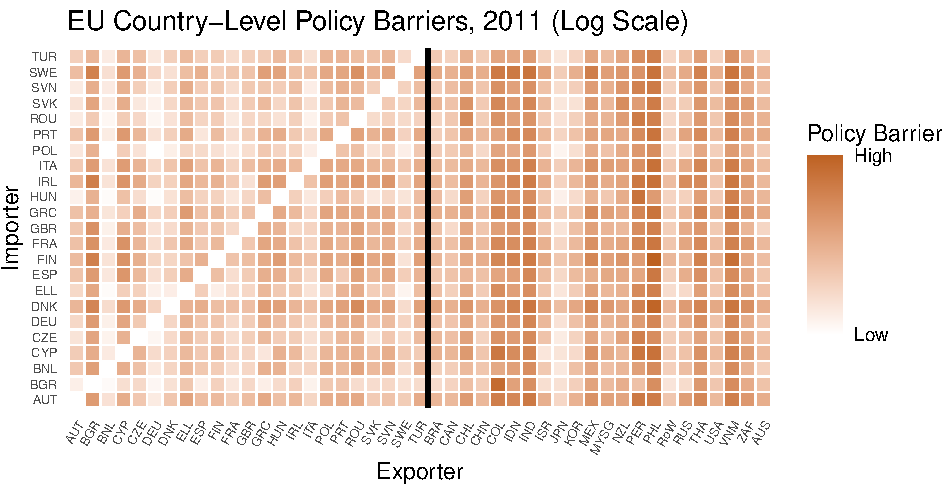
\includegraphics{figure/hmEUD-1.pdf}
\caption{Intra and extra-European Union policy barriers to trade. Each
cell reports the magnitude of the policy barrier each EU importing
country (y-axis) imposes on every exporting country (x-axis). Barriers
toward EU countries are on the left hand side of the solid line.
Barriers toward non-EU countries are on the right hand side of the solid
line. BNL is an aggregate of Belgium, Luxembourg, and the Netherlands
(Benelux). ELL is an aggregate of the Baltic countries: Estonia, Latvia,
and Lithuania. \label{fig:hmEUD}}
\end{figure}

Figure \ref{fig:hmEUD} depicts the results of this exercise.\footnote{In
  Appendix D, I reproduce Figure \ref{fig:hm} with the European Union
  disaggregated and re-implement K-means clustering, with \(K=\) 4. The
  Asian and American blocs remain largely intact. The clustering
  uncovers 2 distinct European blocs -- a Western bloc consisting of
  Great Britain,France, Germany, and their neighbors as well as an
  Eatern bloc consisting of mostly post-Cold War EU entrants.
  Interestingly, Russia and Turkey are grouped with the Western bloc,
  rather than the more geographically proximate Eastern countries.} EU
policy barriers toward other EU member states are on average 56 percent
the size of barriers with non-EU states.\footnote{This comparison was
  made by taking weighted means of tariff-equivalent policy barriers
  where the weights are the expenditures on tradable goods of the
  exporting countries.} Barriers are far from nonexistent, however. On
average, EU countries implement a tariff-equivalent barrier of 69
percent on other EU member states, compared to 119 percent on non-EU
states.\footnote{These are unweighted averages of EU member states'
  TRIs, calculated with respect to EU and non-EU members respectively.}
From the perspective of the model, there remained substantial
policy-related trade frictions within the EU in 2011. This finding is
consistent with the existence of ``border effects'' within the EU
(Comerford and Mora 2015). Of course, these inferences might be driven
by features of the model itself. I discuss these limitations in more
detail in the paper's conclusion.

\subsection{Discussion}

In the introduction, I noted that richer countries tend to have higher
policy barriers to trade, contrary to their relatively liberal tariff
regimes. From this fact, some conclude that political institutions in
developed countries are more ``welfare-conscious'' than those in their
developing counterparts (Gawande, Krishna, and Olarreaga 2009, 2015).
These results are consistent with an alternative approach, emphasizing
state capacity, articulated in Acemoglu (2005), Rodrik (2008), and
Queralt (2015). Here, tariffs emerge as a ``second-best'' solution to a
revenue-raising problem facing low-capacity governments, which struggle
to raise revenue through other channels. As capacity grows, governments
employ alternative instruments to raise revenues. As shown here, these
governments do not necessarily become less protectionist in the process.
In fact, they may become more closed to international trade.

\begin{figure}
\centering
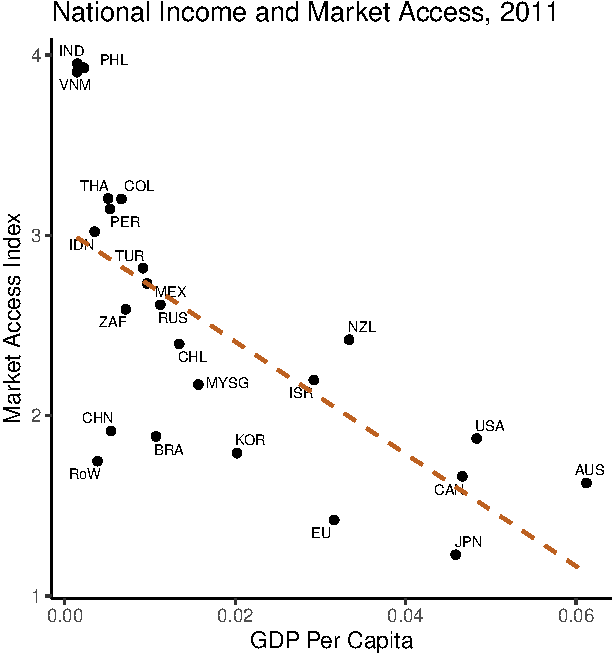
\includegraphics{figure/maiGdppc-1.pdf}
\caption{Market access conditions and per capita national income
\label{fig:maiGdppc}}
\end{figure}

Due to the restrictiveness and discrimination inherent in developed
countries' trade policies, poor countries also struggle to access
international markets, shown in Figure \ref{fig:maiGdppc}. Several
studies examining trade costs as a whole replicate this finding, and
suggest that this explains some of the variation in cross-national
income per capita (Redding and Venables 2004; Romalis 2007; Waugh 2010).
These results suggest that even complete tariff liberalization on the
part of developed countries would still leave developing countries
confronting substantial market access barriers.

\section{Conclusion}

The structure of global tariff rates suggests that international trade
is relatively free and fair. Does this conclusion extend to non-tariff
barriers to trade? I have shown that the policy barriers to trade
implied by observed prices, trade flows, and freight costs are quite
large and are implemented in a discriminatory manner. In particular,
developed countries implement high non-tariff barriers to trade and tend
to discriminate against their less-developed trading partners.

I should qualify these conclusions on three counts. First, like most
studies of international trade, they are model-dependent. My approach
accounts for trade in intermediate inputs, but does so rather bluntly.
Global value chains are complex and respond non-linearly to changes in
trade costs (Yi 2003), a feature not captured here. The nested CES
preferences ascribed to consumers are also rather rigid. This
inflexibility may affect the proportion of distortions attributed to
trade costs, rather than consumer heterogeneity, a point noted by Waugh
(2010). Second, my conclusions depend on the accuracy of the ICP's price
data, and on the assumption that producers face the same prices as
consumers. If the price level in Japan is factually less than twice that
of Malaysia, Japan's implied policy barriers to trade will also fall.
Similarly, if intermediate input prices differ systematically from the
prices of final goods, this will change my conclusions on the magnitude
of policy barriers to trade. Finally, the simple calibration exercise
conducted here cannot speak to uncertainty about the magnitude of policy
barriers to trade. From the perspective of Equation \ref{eq:tau},
measurement error in prices and trade flows and estimation error in the
trade elasticity and predicted trade costs will aggregate to produce a
window of uncertainty the true value of \(\tau_{ij}\). Some combination
of better theory and better data will strengthen the precision of the
conclusions made here.

\clearpage

\section{Appendix}

\subsection{A: Empirical Price Index: Estimating Consumers' Price
Elasticity and Taste Parameters}

Demand for variety \(\omega\) is \[
q_i(\omega) = \tilde{\alpha}_{i, h(\omega)} p_i(\omega)^{-\sigma} E_i^q P_i^{\sigma - 1}
\] and expenditure is \[
x_i(\omega) = p_i(\omega) q_i(\omega) = \tilde{\alpha}_{i, h(\omega)} p_i(\omega)^{1-\sigma} E_i^q P_i^{\sigma - 1} . 
\]

With constant prices in each basic heading, total spending on goods in
category \(k\) is \begin{align*}
x_{ik} &= \int_{\omega \in \Omega_k} \tilde{\alpha}_{i, h(\omega)} p_i(\omega)^{1-\sigma} E_i^q P_i^{\sigma - 1} d \omega \\
&= \int_{\omega \in \Omega_k} \tilde{i, \alpha}_k p_{ik}^{1 - \sigma} E_i^q P_i^{\sigma - 1} d \omega \\
&= \frac{1}{K} \tilde{\alpha}_{ik} p_{ik}^{1 - \sigma} E_i^q P_i^{\sigma - 1}
\end{align*} and the share of \(i\)'s tradables expenditure spent on
goods in category \(k\) is \[
\lambda_{ik} = \frac{x_{ik}}{E_i^q} = \frac{1}{K} \tilde{\alpha}_{ik} p_{ik}^{1 - \sigma} P_i^{\sigma - 1} .
\]

With the United States as the base country, \(p_{\text{US}, k} = 1\) for
all \(k\). Differencing by \(\lambda_{\text{US}, k}\) then gives
\begin{align*}
\frac{\lambda_{ik}}{\lambda_{\text{US}, k}} &= \frac{\tilde{\alpha}_{ik}}{\tilde{\alpha}_{\text{US}, k}} p_{ik}^{1-\sigma} P_i^{\sigma - 1}
\\
&= \frac{\epsilon_{ik}}{\epsilon_{\text{US},k}} p_{ik}^{1-\sigma} P_i^{\sigma - 1}
\end{align*} where I enforce the normalization that \(P_{US} = 1\).
Taking logs, \[
\ln \left( \frac{\lambda_{ik}}{\lambda_{\text{US}, k}} \right) = \ln \left( \frac{\epsilon_{ik}}{\epsilon_{\text{US},k}} \right) + (1 - \sigma) \ln \left( p_{ik} \right) + (\sigma - 1) \ln \left( P_i \right)
\] which can be rearranged as \[
\ln p_{ik} = \frac{1}{1 - \sigma} \ln \left( \frac{\lambda_{ik}}{\lambda_{\text{US}, k}} \right) + \ln \left( P_i \right) + \frac{1}{\sigma - 1} \ln \left( \frac{\epsilon_{ik}}{\epsilon_{\text{US},k}} \right) .
\] Because \(\E [ \epsilon_{ik} ] = 1\), \[
\E \left[ \ln p_{ik} \right] = \frac{1}{1 - \sigma} \ln \left( \frac{\lambda_{ik}}{\lambda_{\text{US}, k}} \right) + \ln \left( P_i \right) 
\] which gives a moment condition that I estimate via ordinary least
squares.

\subsection{B: Modeling Freight Costs}

I build a simple model of demand for transportation services in order to
estimate freight costs. There are \(M\) sectors, indexed
\(m \in \left\{ 1, ..., M \right\}\) and \(K\) modes of transportation
(air, sea, land), indexed \(k \in \left\{ 1, ..., K \right\}\). There is
a mass of exporters within each country-sector. The cost of shipping a
good from sector \(m\) from country \(i\) to country \(j\) via mode
\(k\) is \(\delta_{ij}^{mk}(\bm{Z}_ij)\) where \(\bm{Z}_{ij}\) is a
vector storing geographic covariates including indicators of air and sea
distances between \(i\) and \(j\), and whether or not \(i\) and \(j\)
are contiguous.

Exporters have preferences over the mode of transit and cost of freight.
Let \[
V_{ij}^{mk} = \tilde{\beta}_0 \delta_{ij}^{mk}(\bm{Z}_{ij}) + \tilde{\beta}_k + \eta_{ij}^{km}
\] where \(\eta_{ij}^{km}\) is a Type-I extreme value-distributed
preference shock with \(\E [\eta_{ij}^{km}] = 0\). \(\tilde{\beta}_k\)
modulates exporters' relative preference for mode \(k\), independent of
its cost. This is a simple logit model of mode choice a la Mcfadden
(1974). Under these assumptions, the share of exporters in sector \(k\)
that choose to ship from \(j\) to \(i\) via mode \(m\) is
\begin{equation} \label{eq:logitShares}
\zeta_{ij}^{m k} = \frac{\exp \left( \tilde{\beta}_0 \delta_{ij}^{mk}(\bm{Z}_{ij}) + \tilde{\beta}_k \right)}{\sum_{k^\prime=1}^K \exp \left( \tilde{\beta}_0 \delta_{ij}^{mk^\prime}(\bm{Z}_{ij}) + \tilde{\beta}_{k^\prime} \right)} .
\end{equation} I impose natural technological constraints on this
function, prohibiting shipment by sea to landlocked countries and
shipment by land to islands or across continents.\footnote{Where Eurasia
  is treated as an aggregate.}

I model \(\delta_{ij}^{mk}(\bm{Z}_{ij})\) as linear in distance and
contiguity and sector (HS2) fixed effects.\footnote{I also smooth the
  model's predictions over years using a polynomial spline.} Parameter
estimates for each mode are reported in the next section.

I obtain estimates for \(\tilde{\beta}_0\) and \(\tilde{\beta}_k\) by
taking the log of \ref{eq:logitShares}, differencing with respect to a
base transportation mode, and estimating the resulting linear equation
via ordinary least squares. With parameter estimates in hand, I can
compute predictions for total trade costs by aggregating over sectors
and projecting out of sample.

The total free on board (f.o.b.) value of imports of country \(i\) from
country \(j\) is given by \(X_{ij}\). The cost, insurance, and freight
(c.i.f.) value of these goods is \(\delta_{ij} X_{ij}\). These c.i.f.
costs can be decomposed by product and mode of transportation as follows
\[
\delta_{ij} X_{ij} = \sum_{m = 1}^M \delta_{ij}^m x_{ij}^m
\] where \[
\delta_{ij}^m x_{ij}^m = \sum_{k=1}^K \delta_{ij}^{m k} x_{ij}^{m k} \implies \delta_{ij}^m =  \sum_{k=1}^K \delta_{ij}^{m k} \frac{x_{ij}^{m k}}{x_{ij}^m} .
\]

Recall that \(\zeta_{ij}^{m k}\) is the share of imports by \(i\) from
\(j\) of good \(m\) that travel by mode \(k\) \[
\zeta_{ij}^{m k} = \frac{x_{ij}^{m k}}{x_{ij}^m} .
\]

With these terms defined, total predicted freight costs can be computed
as \[
\hat{\delta}_{ij} \left( \bm{Z}_{ij} \right) = \frac{1}{X_{ij}} \sum_{m = 1}^M x_{ij}^m \sum_{k=1}^K \zeta_{ij}^{m k}\left( \delta_{ij}^{mk}(\bm{Z}_{ij}) \right) \delta_{ij}^{mk}(\bm{Z}_{ij}) .
\]

\subsection{C: Freight Cost Data Sources and Results}

To estimate freight costs and mode share choice, I employ data from the
United States Census Bureau and the Australian Bureau of Statistics on
the c.i.f. and f.o.b. values of its imports.\footnote{The Australian
  data are also used by Shapiro (2016) and Adao, Costinot, and Donaldson
  (2017).} The ratio of the c.i.f. value of goods to their f.o.b. value
can then be taken as a measure of the ad valorem freight cost. I
supplement these values with international data on the costs of
\emph{maritime} shipments from the OECD's
\href{https://doi.org/10.1787/data-00490-en}{Maritime Transport Cost
Dataset} (Korinek 2011). I also observe the transportation modes of
imports (air, land, or sea) to the European Union, Japan, Brazil,
Australia and the United States .\footnote{Data from the United States
  come from the Census Bureau and are available on the website of
  \href{http://faculty.som.yale.edu/peterschott/sub_international.htm}{Peter
  Schott}. Data from the European Union are from
  \href{https://ec.europa.eu/eurostat}{Eurostat}. Data from Japan are
  from the government's statistical agency,
  \href{https://www.e-stat.go.jp/en/stat-search/files?page=1\&toukei=00350300\&bunya_l=16\&tstat=000001013142\&result_page=1\&second=1}{e-Stat}.
  Data from Brazil come from the
  \href{http://comexstat.mdic.gov.br/en/home}{ministry of trade and
  industry}. Data from Australia are from the Australian Bureau of
  Statistics.}

To model the cost of transport via sea, I take sea distances from
\href{http://www.ferdi.fr/en/indicator/cerdi-seadistance-database}{CERDI}
(Bertoli, Goujon, and Santoni 2016). For land and air distances, I use
CEPII's
\href{http://www.cepii.fr/cepii/en/bdd_modele/presentation.asp?id=6}{GeoDist}
database (Mayer and Zignago 2011).

Parameter estimates for mode-specific freight cost models are reported
in the following three tables. Across modes, distance is estimated to
significantly increase freight costs. Contiguity is estimated to
decrease costs for land and air shipments while increasing costs for
seaborne shipments.

\subsubsection{Maritime Freight Costs}

\begin{table}[!htbp] \centering 
  \caption{Maritime Cost Model} 
  \label{} 
\begin{tabular}{@{\extracolsep{5pt}}lc} 
\\[-1.8ex]\hline 
\hline \\[-1.8ex] 
 & \multicolumn{1}{c}{\textit{Dependent variable:}} \\ 
\cline{2-2} 
\\[-1.8ex] & Freight Cost \\ 
\hline \\[-1.8ex] 
 CERDI seadist (log, std) & 0.010$^{***}$ \\ 
  & (0.0002) \\ 
  & \\ 
 Contiguity & 0.013$^{***}$ \\ 
  & (0.0004) \\ 
  & \\ 
\hline \\[-1.8ex] 
Product fixed effects? & \checkmark \\ 
Cubic time spline? & \checkmark \\ 
Observations & 156,135 \\ 
R$^{2}$ & 0.388 \\ 
\hline 
\hline \\[-1.8ex] 
\textit{Note:}  & \multicolumn{1}{r}{$^{*}$p$<$0.1; $^{**}$p$<$0.05; $^{***}$p$<$0.01} \\ 
\end{tabular} 
\end{table}

\FloatBarrier

\subsubsection{Land Freight Costs}

\begin{table}[!htbp] \centering 
  \caption{Land Cost Model} 
  \label{} 
\begin{tabular}{@{\extracolsep{5pt}}lc} 
\\[-1.8ex]\hline 
\hline \\[-1.8ex] 
 & \multicolumn{1}{c}{\textit{Dependent variable:}} \\ 
\cline{2-2} 
\\[-1.8ex] & Freight Cost \\ 
\hline \\[-1.8ex] 
 CEPII distw (log, std) & 0.003$^{***}$ \\ 
  & (0.0003) \\ 
  & \\ 
 Contiguity & $-$0.016$^{***}$ \\ 
  & (0.001) \\ 
  & \\ 
\hline \\[-1.8ex] 
Product fixed effects? & \checkmark \\ 
Cubic time spline? & \checkmark \\ 
Observations & 26,455 \\ 
R$^{2}$ & 0.500 \\ 
\hline 
\hline \\[-1.8ex] 
\textit{Note:}  & \multicolumn{1}{r}{$^{*}$p$<$0.1; $^{**}$p$<$0.05; $^{***}$p$<$0.01} \\ 
\end{tabular} 
\end{table}

\FloatBarrier

\subsubsection{Air Freight Costs}

\begin{table}[!htbp] \centering 
  \caption{Air Cost Model} 
  \label{} 
\begin{tabular}{@{\extracolsep{5pt}}lc} 
\\[-1.8ex]\hline 
\hline \\[-1.8ex] 
 & \multicolumn{1}{c}{\textit{Dependent variable:}} \\ 
\cline{2-2} 
\\[-1.8ex] & Freight Cost \\ 
\hline \\[-1.8ex] 
 CEPII distw (log, std) & 0.028$^{***}$ \\ 
  & (0.001) \\ 
  & \\ 
 Contiguity & $-$0.030$^{***}$ \\ 
  & (0.002) \\ 
  & \\ 
\hline \\[-1.8ex] 
Product fixed effects? & \checkmark \\ 
Cubic time spline? & \checkmark \\ 
Observations & 58,346 \\ 
R$^{2}$ & 0.351 \\ 
\hline 
\hline \\[-1.8ex] 
\textit{Note:}  & \multicolumn{1}{r}{$^{*}$p$<$0.1; $^{**}$p$<$0.05; $^{***}$p$<$0.01} \\ 
\end{tabular} 
\end{table}

\FloatBarrier

\subsubsection{Transportation Mode Shares}

With \(\delta_{ij}(\bm{Z}_{ij})\) estimated I can compute predicted
sector-level freight costs for all country pairs. I use these predicted
freight prices to estimate the parameters of the mode choice model,
using all observed mode share choices.

I take air transport as the baseline category for the transportation
modes model. Price increases in mode \(k\) are estimated to decrease
that mode's relative market share. Sea is estimated to be the most
popular mode, holding prices fixed, followed by air and land
respectively. Holding these preferences (captured in
\(\tilde{\beta}_k\)) fixed at estimated values for all modes and
assuming transport via all modes is equally costly, a one percent
increase in the relative cost of seaborne trade decreases its expected
market share from 70.7 percent to 68.8 percent.

\begin{table}[!htbp] \centering 
  \caption{Mode Share Model} 
  \label{} 
\begin{tabular}{@{\extracolsep{5pt}}lc} 
\\[-1.8ex]\hline 
\hline \\[-1.8ex] 
 & \multicolumn{1}{c}{\textit{Dependent variable:}} \\ 
\cline{2-2} 
\\[-1.8ex] & (Log) Relative Share \\ 
\hline \\[-1.8ex] 
 Predicted Price Ratio & $-$9.039$^{***}$ \\ 
  & (0.090) \\ 
  & \\ 
 Sea FE & 1.115$^{***}$ \\ 
  & (0.013) \\ 
  & \\ 
 Land FE & $-$1.338$^{***}$ \\ 
  & (0.017) \\ 
  & \\ 
\hline \\[-1.8ex] 
Observations & 145,846 \\ 
R$^{2}$ & 0.263 \\ 
\hline 
\hline \\[-1.8ex] 
\textit{Note:}  & \multicolumn{1}{r}{$^{*}$p$<$0.1; $^{**}$p$<$0.05; $^{***}$p$<$0.01} \\ 
\end{tabular} 
\end{table}

\FloatBarrier

\subsection{D: Economic Blocs, Disaggregated European Union}

\begin{figure}
\centering
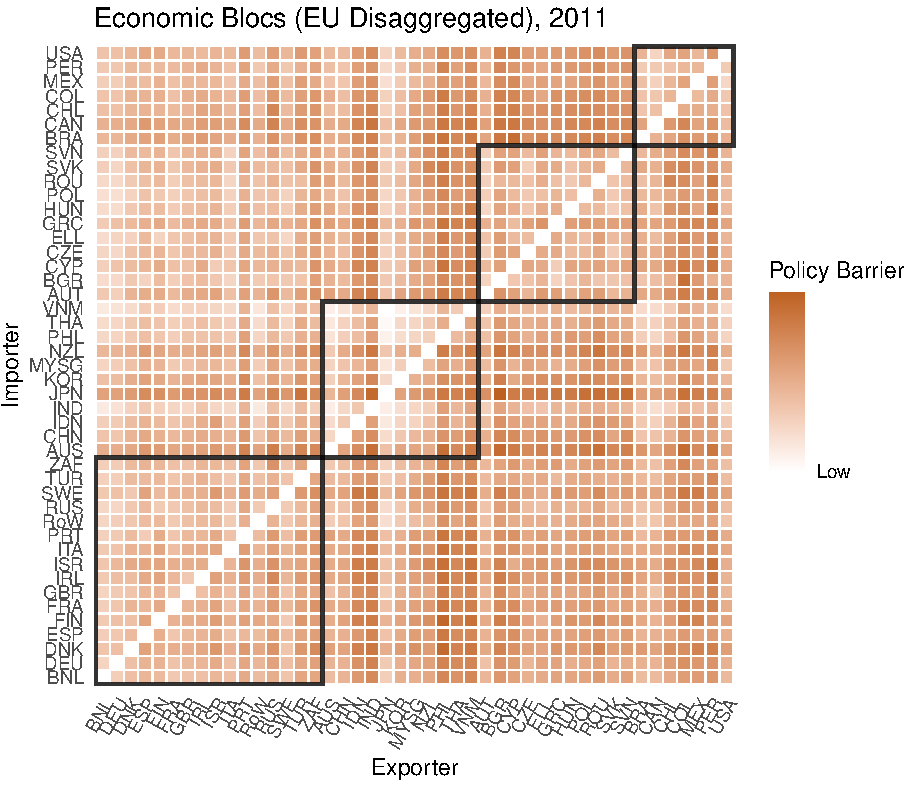
\includegraphics{figure/hmEUDC-1.pdf}
\caption{Distribution of policy barriers to trade with individual EU
countries. Each cell reports the magnitude of the policy barrier each
importing country (y-axis) imposes on every exporting country (x-axis).
Countries are partitioned into 4 groups through K-means clustering.
Black rectangles enclose each cluster.}
\end{figure}

\FloatBarrier

\subsection{E: Sample Countries}

\begingroup\fontsize{9}{11}\selectfont

\begin{longtable}{ll}
\toprule
iso3 & Country Name\\
\midrule
\endfirsthead
\multicolumn{2}{@{}l}{\textit{(continued)}}\\
\toprule
iso3 & Country Name\\
\midrule
\endhead
\
\endfoot
\bottomrule
\endlastfoot
AUS & Australia\\
BRA & Brazil\\
CAN & Canada\\
CHL & Chile\\
CHN & China\\
\addlinespace
COL & Colombia\\
EU & European Union\\
IDN & Indonesia\\
IND & India\\
ISR & Israel\\
\addlinespace
JPN & Japan\\
KOR & South Korea\\
MEX & Mexico\\
MYSG & NA\\
NZL & New Zealand\\
\addlinespace
PER & Peru\\
PHL & Philippines\\
RoW & Rest of the World\\
RUS & Russia\\
THA & Thailand\\
\addlinespace
TUR & Turkey\\
USA & United States\\
VNM & Vietnam\\
ZAF & South Africa\\*
\end{longtable}
\endgroup{}

\subsection{F: International Comparison Program Expenditure Categories}

\begingroup\fontsize{9}{11}\selectfont

\begin{longtable}{rll}
\toprule
Code & Basic Heading & Tradable?\\
\midrule
\endfirsthead
\multicolumn{3}{@{}l}{\textit{(continued)}}\\
\toprule
Code & Basic Heading & Tradable?\\
\midrule
\endhead
\
\endfoot
\bottomrule
\endlastfoot
1101111 & Rice & \checkmark\\
1101112 & Other cereals, flour and other products & \checkmark\\
1101113 & Bread & \checkmark\\
1101114 & Other bakery products & \checkmark\\
1101115 & Pasta products & \checkmark\\
\addlinespace
1101121 & Beef and veal & \checkmark\\
1101122 & Pork & \checkmark\\
1101123 & Lamb, mutton and goat & \checkmark\\
1101124 & Poultry & \checkmark\\
1101125 & Other meats and meat preparations & \checkmark\\
\addlinespace
1101131 & Fresh, chilled or frozen fish and seafood & \checkmark\\
1101132 & Preserved or processed fish and seafood & \checkmark\\
1101141 & Fresh milk & \checkmark\\
1101142 & Preserved milk and other milk products & \checkmark\\
1101143 & Cheese & \checkmark\\
\addlinespace
1101144 & Eggs and egg-based products & \checkmark\\
1101151 & Butter and margarine & \checkmark\\
1101153 & Other edible oils and fats & \checkmark\\
1101161 & Fresh or chilled fruit & \checkmark\\
1101162 & Frozen, preserved or processed fruit and fruit-based products & \checkmark\\
\addlinespace
1101171 & Fresh or chilled vegetables other than potatoes & \checkmark\\
1101172 & Fresh or chilled potatoes & \checkmark\\
1101173 & Frozen, preserved or processed vegetables and vegetable-based products & \checkmark\\
1101181 & Sugar & \checkmark\\
1101182 & Jams, marmalades and honey & \checkmark\\
\addlinespace
1101183 & Confectionery, chocolate and ice cream & \checkmark\\
1101191 & Food products nec & \checkmark\\
1101211 & Coffee, tea and cocoa & \checkmark\\
1101221 & Mineral waters, soft drinks, fruit and vegetable juices & \checkmark\\
1102111 & Spirits & \checkmark\\
\addlinespace
1102121 & Wine & \checkmark\\
1102131 & Beer & \checkmark\\
1102211 & Tobacco & \checkmark\\
1102311 & Narcotics & \\
1103111 & Clothing materials, other articles of clothing and clothing accessories & \checkmark\\
\addlinespace
1103121 & Garments & \checkmark\\
1103141 & Cleaning, repair and hire of clothing & \\
1103211 & Shoes and other footwear & \checkmark\\
1103221 & Repair and hire of footwear & \\
1104111 & Actual and imputed rentals for housing & \\
\addlinespace
1104311 & Maintenance and repair of the dwelling & \\
1104411 & Water supply & \\
1104421 & Miscellaneous services relating to the dwelling & \\
1104511 & Electricity & \checkmark\\
1104521 & Gas & \checkmark\\
\addlinespace
1104531 & Other fuels & \checkmark\\
1105111 & Furniture and furnishings & \checkmark\\
1105121 & Carpets and other floor coverings & \checkmark\\
1105131 & Repair of furniture, furnishings and floor coverings & \\
1105211 & Household textiles & \checkmark\\
\addlinespace
1105311 & Major household appliances whether electric or not & \checkmark\\
1105321 & Small electric household appliances & \checkmark\\
1105331 & Repair of household appliances & \\
1105411 & Glassware, tableware and household utensils & \checkmark\\
1105511 & Major tools and equipment & \checkmark\\
\addlinespace
1105521 & Small tools and miscellaneous accessories & \checkmark\\
1105611 & Non-durable household goods & \checkmark\\
1105621 & Domestic services & \\
1105622 & Household services & \\
1106111 & Pharmaceutical products & \checkmark\\
\addlinespace
1106121 & Other medical products & \checkmark\\
1106131 & Therapeutic appliances and equipment & \checkmark\\
1106211 & Medical Services & \\
1106221 & Dental services & \\
1106231 & Paramedical services & \\
\addlinespace
1106311 & Hospital services & \\
1107111 & Motor cars & \checkmark\\
1107121 & Motor cycles & \checkmark\\
1107131 & Bicycles & \checkmark\\
1107141 & Animal drawn vehicles & \checkmark\\
\addlinespace
1107221 & Fuels and lubricants for personal transport equipment & \checkmark\\
1107231 & Maintenance and repair of personal transport equipemnt & \\
1107241 & Other services in respect of personal transport equipment & \\
1107311 & Passenger transport by railway & \\
1107321 & Passenger transport by road & \\
\addlinespace
1107331 & Passenger transport by air & \\
1107341 & Passenger transport by sea and inland waterway & \\
1107351 & Combined passenger transport & \\
1107361 & Other purchased transport services & \\
1108111 & Postal services & \\
\addlinespace
1108211 & Telephone and telefax equipment & \checkmark\\
1108311 & Telephone and telefax services & \\
1109111 & Audio-visual, photographic and information processing equipment & \checkmark\\
1109141 & Recording media & \checkmark\\
1109151 & Repair of audio-visual, photographic and information processing equipment & \\
\addlinespace
1109211 & Major durables for outdoor and indoor recreation & \checkmark\\
1109231 & Maintenance and repair of other major durables for recreation and culture & \\
1109311 & Other recreational items and equipment & \checkmark\\
1109331 & Garden and pets & \\
1109351 & Veterinary and other services for pets & \\
\addlinespace
1109411 & Recreational and sporting services & \\
1109421 & Cultural services & \\
1109431 & Games of chance & \\
1109511 & Newspapers, books and stationery & \checkmark\\
1109611 & Package holidays & \\
\addlinespace
1110111 & Education & \\
1111111 & Catering services & \\
1111211 & Accommodation services & \\
1112111 & Hairdressing salons and personal grooming establishments & \\
1112121 & Appliances, articles and products for personal care & \checkmark\\
\addlinespace
1112211 & Prostitution & \\
1112311 & Jewellery, clocks and watches & \checkmark\\
1112321 & Other personal effects & \checkmark\\
1112411 & Social protection & \\
1112511 & Insurance & \\
\addlinespace
1112611 & Financial Intermediation Services Indirectly Measured (FISIM) & \\
1112621 & Other financial services & \\
1112711 & Other services nec & \\
1113111 & Final consumption expenditure of resident households in the rest of the world & \\
1113112 & Final consumption expenditure of non-resident households in the economic territory & \\
\addlinespace
1201111 & Individual consumption expenditure by NPISHs & \\
1301111 & Housing & \\
1302111 & Pharmaceutical products & \checkmark\\
1302112 & Other medical products & \checkmark\\
1302113 & Therapeutic appliances and equipment & \checkmark\\
\addlinespace
1302121 & Out-patient medical services & \\
1302122 & Out-patient dental services & \\
1302123 & Out-patient paramedical services & \\
1302124 & Hospital services & \\
1302211 & Compensation of employees & \\
\addlinespace
1302221 & Intermediate consumption & \\
1302231 & Gross operating surplus & \\
1302241 & Net taxes on production & \\
1302251 & Receipts from sales & \\
1303111 & Recreation and culture & \\
\addlinespace
1304111 & Education benefits and reimbursements & \\
1304211 & Compensation of employees & \\
1304221 & Intermediate consumption & \\
1304231 & Gross operating surplus & \\
1304241 & Net taxes on production & \\
\addlinespace
1304251 & Receipt from sales & \\
1305111 & Social protection & \\
1401111 & Compensation of employees & \\
1401121 & Intermediate consumption & \\
1401131 & Gross operating surplus & \\
\addlinespace
1401141 & Net taxes on production & \\
1401151 & Receipts from sales & \\
1501111 & Fabricated metal products, except machinery and equipment & \checkmark\\
1501121 & General purpose machinery & \checkmark\\
1501131 & Special purpose machinery & \checkmark\\
\addlinespace
1501141 & Electrical and optical equipment & \checkmark\\
1501151 & Other manufactured goods nec & \checkmark\\
1501211 & Motor vehicles, trailers and semi-trailers & \checkmark\\
1501212 & Other road transport & \checkmark\\
1501221 & Other transport equipment & \checkmark\\
\addlinespace
1502111 & Residential buildings & \\
1502211 & Non-residential buildings & \\
1502311 & Civil engineering works & \\
1503111 & Other products & \\
1601111 & Opening value of inventories & \\
\addlinespace
1601112 & Closing value of inventories & \\
1602111 & Acquisitions of valuables & \\
1602112 & Disposals of valuables & \\
1701111 & Exports of goods and services & \\
1701112 & Imports of goods and services & \\*
\end{longtable}
\endgroup{}

\clearpage

\chapter[Trade Policy in the Shadow of Power: Quantifying Military Coercion in the International System]{Trade Policy in the Shadow of Power \\ \Large Quantifying Military Coercion in the International System}

\section{Introduction}

Military power holds a central position in international relations (IR)
theory. Governments exist in a state of anarchy --- there is no world
authority tasked with preventing the use of violence in settling
policies disputes between them. As a result, powerful governments can
employ force against others to secure more favorable policy outcomes.
This does not necessarily imply that international relations are
uniquely violent, however. Threatened governments can adjust their
policy choices to accommodate the interests of the powerful, avoiding
costly conflict (Brito and Intrilagator 1985; Fearon 1995). This setting
raises an inference problem --- do observed policies reflect the
preferences of the governments that adopted them, or the military
constraints of the anarchic international system?

In this paper, I propose and implement a method to assess the effect of
military power on trade policy choices. Trade is a natural issue area in
which to undertake such an investigation. For a variety of reasons,
governments' endeavor to protect their home market to some extent.
Governments also seek access to foreign markets (Grossman 2016). These
preferences put governments into conflict with one another -- each would
like to erect some barriers to imports while dismantling barriers to
trade abroad. Given dictatorial power, governments would protect their
home market and enforce openness elsewhere. Moreover, aggregate
policy-induced trade frictions are large (Cooley 2019a) and have large
effects on the distribution and level of welfare within and across
countries (Autor, Dorn, and Hanson 2013; Costinot and Rodríguez-Clare
2015; Goldberg and Pavcnik 2016). These effects may be particularly
salient for politically influential groups (Grossman and Helpman 1994;
Osgood et al. 2017). Governments therefore have incentives to use force
to shape trade policy abroad to their liking. Historically, they have
been willing to fight wars to realize such goals (Findlay and O'Rourke
2007).

Assessing the effect of military power on trade policy requires
imagining what policy choices governments would have made in the absence
of coercion. Uncoerced policies can be taken as a measure of the
government's ideal point, representing its true underlying preferences.
When coercion is possible, however, weaker governments must consider the
effect of their policy choices on the powerful. If a particular policy
choice harms a threatening government enough, it can choose to impose an
alternative policy by force. Recognizing this threat, weaker governments
adjust their policies to avoid war. In an anarchic world, policies are
jointly determined by both power and preferences.

I proceed in three steps to untangle power and preferences as
determinants of trade policies. First, I model a coercive international
political economy in which governments propose trade policies, observe
others proposals, and choose whether or not to fight wars to win the
right to modify these. The model's equilibrium depends on a vector of
parameters governing governments' preferences for protectionism and
costs of war, which in turn depend on the military strengths of
potential belligerents and the geographic distance between them. I then
estimate these parameters by minimizing the distance between the model's
predictions and observed policies in the year 2011. Finally, I answer
the question posed here: how does military coercion affect trade policy?
With estimates for the model's parameters in hand, this question can be
answered by a simple counterfactual experiment --- eliminate
governments' military capacity, and recalculate the model's equilibrium.
The difference between counterfactual equilibrium policies and the
factual policies represents the net effect of military coercion on trade
policy.

I find that there are increasing returns to military advantage in
international trade policy bargaining. Governments that are militarily
powerful are estimated to enjoy lower costs of war, which they exploit
to coerce policy concessions from their trade partners. In this sense,
military might is a force for trade liberalization, inducing reductions
in barriers to trade that governments would be unwilling to undertake in
the absence of coercion. These reductions in barriers to trade stimulate
international economic exchange. Counterfactually eliminating militaries
reduces the value of global trade to 61.4 percent of its model-estimated
value. I estimate that the effectiveness of military coercion does not
degrade across space -- in fact, governments are estimated to enjoy
lower average costs of war against geographically distant adversaries.
This may reflect the peculiarities of the technology of war in the era
under study, in which geographic distance represents a minimal
impediment to the projection of power.

In the model, governments choose trade policies to maximize a
country-specific social welfare function. Each government's trade policy
is a set of taxes, one for each importing country, imposed on imports.
Notably, trade policies can be discriminatory, affecting certain source
countries disproportionately. A model of the international economy
connects trade policy choices to social welfare.\footnote{The model of
  the international economy is a variant of the workhorse model of Eaton
  and Kortum (2002). Costinot and Rodríguez-Clare (2015) study a broader
  class of structural gravity models that connect trade frictions (such
  as trade policy) to trade and welfare outcomes.} After observing trade
policies, governments may choose to fight wars against other governments
in order to impose free trade. The threat of war constrains threatened
governments and affects their trade policy choices. The dyadic costs of
war, held as private information to potential attackers, depend on
observable features of the attacking and defending countries, including
the potential belligerents' relative military strengths' and the
geographic distance between them. Governments' ideal policies depend on
a country-specific parameter governing the ease with which policy
distortions are converted into revenues. I show that these preference
parameters and the elasticities that convert military strength and
geographic distance into war costs can be estimated given data on
directed policy barriers to trade -- or the magnitude of policy
distortion each government imposes on imposes on imports from each other
country.\footnote{I use data on aggregate directed trade policy
  distortions from Cooley (2019a), a companion paper to this study.
  These data are discussed in more detail below.}

Within-country variation in trade policy identifies the model. Consider
the ideal set of trade policies of a government whose preferences are
known. The policies that achieve this objective can be readily
calculated given knowledge of parameters governing international
economic relations. Policies adopted toward imports from countries that
pose no military threat will reflect this objective. Conversely, the
imports of threatening countries will encounter lower barriers to trade,
in order to satisfy the threatener's war constraint. This favoritism is
informative about the effectiveness of military threats. The level of
barriers toward non-threatening countries is informative about the
government's preferences. Differential responses to the same level of
threat from different geographic locations identifies parameters
governing the effectiveness of power projection across space.

The identified model enables two classes of counterfactuals. First, it
allows me to quantify the ``shadow of power'' by comparing factual
policies to those that would prevail if governments' counterfactually
possessed zero military capability. These policies can then be fed into
the model of the international economy to calculate the effect on trade
flows, prices, and wages around the world. Would different trade blocs
emerge in a coercion-free world? Which governments would benefit the
most? In the model, consumers benefit from the liberalizing effect of
foreign military coercion (Antràs and Padró i Miquel 2011; Cooley
2019b). How large are these benefits? Whose citizens benefit the most
from international power politics? How would relative changes to U.S.
and Chinese military strength affect the functioning of the
international economy?

I also examine how domestic political economic changes (changes to
government preferences) affect the salience of military coercion.
Governments that value the welfare of consumers prefer to adopt lower
barriers to trade. The returns to coercing these governments are
smaller, because their ideal policies impose relatively small
externalities on potential threatening governments. Military coercion
plays a smaller role in influencing trade policy when governments are
relatively liberal. Domestic political institutions are believed to
affect trade policy preferences (Rodrik 1995; Milner 1999; Milner and
Kubota 2005). The model facilitates exploration of how domestic
political change affects the quality of international relations and
governments' propensity to threaten, display, and use military force
against one another.

\section{Literature}

Conflicts of interest and the specter of coercive diplomacy emerge in
the model due to governments' protectionist preferences. Trade theory
reserves a role for small trade policy distortions for governments that
seek to maximize aggregate societal wealth (Johnson 1953; Broda, Limao,
and Weinstein 2008). Empirically, governments implement larger trade
distortions than predicted in theory, however. This regularity motivated
the study of the political economics of trade policy. While nearly free
trade may be good for a society as a whole, owners of specific factors
of production may prefer protectionism. If these groups have better
access to the policymaking process, trade policy may be more
protectionist than is optimal for society (Mayer 1984; Rogowski 1987;
Grossman and Helpman 1994). A family of studies uses these theoretical
insights to estimate governments' sensitivity to narrow versus diffuse
interests (Goldberg and Maggi 1999; Mitra, Thomakos, and Ulubasoglu
2006; Gawande, Krishna, and Olarreaga 2009, 2012, 2015; Ossa 2014).
Because these models incorporate no theory of international military
coercion, these estimates reflect the assumption that policy choices
reflect the outcome of non-cooperative policy choice or non-militarized
bargaining. Fiscal pressures might also drive protectionism. Some
governments are constrained in their ability to raise revenue through
taxes on domestic economic activities. Tariffs and other trade
distortions may substitute as a revenue-raising strategy in these cases
(Rodrik 2008; Queralt 2015).

I take no stance on the domestic political origins of protectionist
preferences. I induce these by varying the ease with which governments
can collect revenues from trade distortions. Each government is
characterized by a revenue threshold parameter. Trade distortions above
the level of this threshold generate revenue while distortions below
this level require subsidies. Governments with higher threshold
parameters therefore prefer higher barriers to trade, all else equal.
This simple formulation induces heterogeneity in the governments' ideal
levels of protectionism and the magnitude of the externalities they
would impose on other governments when choosing individually optimal
policies.

These externalities motivate the lobbying efforts of domestic special
interests and structure international negotiations over trade policy. In
contemporary political economic accounts, large and productive firms
pressure their own governments to secure market access abroad in order
to increase profit opportunities (Ossa 2012; Osgood 2016; Kim 2017). By
contrast, in my model, lower barriers to trade abroad increase wages at
home (helping consumers) and stimulate trade (increasing revenue).
Modeling government preferences in this manner captures market access
incentives tractably while avoiding ascribing a particular domestic
political process to their origin.

Because of these preferences for foreign trade liberalization,
governments have incentives to influence others' policy choices.
Analyzing governments' foreign policy in the 17th and 18th centuries,
Viner (1948) concludes ``important sources of national wealth\ldots were
available\ldots only to countries with the ability to acquire or retain
them by means of the possession and readiness to use military
strength.'' Powerful governments established colonies and threatened
independent governments in order to shape policy abroad to their liking
(Gallagher and Robinson 1953). While formal empires died quickly after
World War II, softer forms of influence remained. Lake (2013) terms the
resulting order a ``hierarchy'' in which weaker countries exchanged
sovereignty for international political order, provided by a hegemonic
United States. Berger et al. (2013) show that this hierarchy has not
always been benevolent --- U.S. political influence was used to open
markets abroad, a form of ``commercial imperialism.'' An earlier
literature ascribed international economic openness to the presence of
such a hegemon (Krasner 1976; Gilpin 1981; Kindleberger 1986). In
conceptualizing openness as a public good, these theories made stark
predictions about the distribution of military power and the
international economy. In reality, the benefits of changes to trade
policy are quite excludable. The model developed here reflects this
reality by allowing governments to adopt discriminatory trade policies.
Power can therefore be exercised to secure benefits not shared by other
governments. The resulting international economic orders defy
characterization as ``open'' or ``closed.'' In a stylized version of the
model developed here, I show that latent coercive threats can be used to
open foreign markets. Militarily weak countries adopt lower barriers to
trade than their powerful counterparts, all else equal (Cooley 2019b).
Antràs and Padró i Miquel (2011) consider a similar model in which
governments influence elections abroad. Again, this influence has a
liberalizing effect on the foreign government's trade policy.

Nevertheless, debate persists about the efficacy of military power in
achieving economic benefits (Mastanduno 2009; Drezner 2013; Bove, Elia,
and Sekeris 2014; Stokes and Waterman 2017). These studies all confront
the inference problem discussed here --- does economic policy reflect
governments' underlying preferences or the shadow of foreign military
power? When redistribution is an alternative to war and bargaining is
frictionless, war is not necessary to achieve coercive effects (Brito
and Intrilagator 1985; Fearon 1995; Art 1996). I assume that the
effectiveness of military coercion depends on governments' relative
military advantage and the geographic distance between an attacking and
defending country. Existing studies examine wars and militarized
disputes to estimate the relationship between military spending and
geographic distance on coercive capacity.\footnote{On the relationship
  between military expenditure and military power, see Kadera and
  Sorokin (2004), Beckley (2010), Beckley (2018), Carroll and Kenkel
  (2019), and Anders, Fariss, and Markowitz (2020). On the loss of
  strength gradient, see Boulding (1962), Bruce Bueno de Mesquita
  (1980), Diehl (1985), Lemke (1995), Gartzke and Braithwaite (2011),
  and Markowitz and Fariss (2013).} The number of disputes used to fit
these models is relatively small and the nature of military technology
changes over time. This dynamic technology and strategic selection into
wars and disputes may confound estimates of these relationships. While I
study a small sample of countries in a single year in this paper, I
expand the universe of cases that can be used to estimate coercive
capability by examining the responsiveness of policy to foreign threats.

Several studies have examined trade policy bargaining theoretically and
empirically. Grossman and Helpman (1995) extend the protection for sale
model to a two-country bargaining setting. Maggi (1999) and Bagwell and
Staiger (1999) focus on the effect of the institutional context in which
trade policy negotiations take place, relative to an
un-institutionalized baseline. Ossa (2014) and Bagwell, Staiger, and
Yurukoglu (2018b) quantify these theories in structural models. Of
course, the continued functioning of international institutions requires
either a) that complying with the rules of the institution be incentive
compatible for each member state, given others' strategies or b) that an
external authority punish deviations from the institutions' rules
sufficiently to induce compliance (Powell 1994). Given the absence of
such an external authority and the stark international distributional
implications of alternative trade policy regimes, it is natural to
consider how the ability to employ military force colors trade policy
bargaining.

Trade and trade policy are often theorized as tools governments can
leverage to achieve political objectives (Hirschman 1945; Gowa and
Mansfield 1993; Martin, Mayer, and Thoenig 2012; Seitz, Tarasov, and
Zakharenko 2015). Yet, affecting trade policy and concomitant prices,
wages, and trade flows is also a central government objective in
international relations. Moreover, the political objectives that
ostensibly motivate governments in these ``trade as means'' models are
loosely defined (e.g.~``security'') and themselves means to achieving
other ends. Studying trade policy as a strategic end allows the analyst
to leverage a family of empirical methods in international economics to
construct counterfactual trade regimes and analyze their welfare
implications (Eaton and Kortum 2002; Head and Mayer 2014; Costinot and
Rodríguez-Clare 2015; Ossa 2016). Government objectives can be defined
flexibly as a function of general equilibrium outputs (prices, wages,
revenues).

A handful of other theoretical studies examine how power affects
exchange in market environments (Skaperdas 2001; Piccione and Rubinstein
2007; Garfinkel, Skaperdas, and Syropoulos 2011; Carroll 2018). Where
property rights are assumed in classical models of the economy, these
authors consider exchange and violence as coequal means to acquire goods
from others. I instead direct attention to coercive bargaining over
endogenous trade frictions (trade policy). These in turn affect the
distribution of goods and welfare in the international economy.

\section{Data and Calibration of Economy}

I estimate the model on a set of 9 governments in the year
2011.\footnote{Focusing on a small set of governments is necessary for
  computational tractability. However, the largest countries (by GDP)
  are the most attractive targets for coercion, as changes to their
  trade policies return the largest welfare gains.} These governments
are listed in Table \ref{tab:ccodes}. I aggregate all European Union
governments into a single entity and collapse all countries not included
in the analysis into a ``Rest of World'' (RoW) aggregate.\footnote{Such
  an aggregation is necessary in order to calculate fully general
  equilibrium effects of counterfactual trade policies. However, I
  prohibit other countries from invading RoW and likewise prohibit RoW
  from invading others. This ensures that estimates of military
  parameters depend almost entirely on interactions between countries
  within my sample.} Non-RoW countries make up 72 percent of world GDP.

\begin{table}

\caption{\label{tab:ccodes}In-Sample Countries \label{tab:ccodes}}
\centering
\begin{tabular}[t]{ll}
\toprule
iso3 & Country Name\\
\midrule
\cellcolor{gray!6}{AUS} & \cellcolor{gray!6}{Australia}\\
CAN & Canada\\
\cellcolor{gray!6}{CHN} & \cellcolor{gray!6}{China}\\
EU & European Union\\
\cellcolor{gray!6}{JPN} & \cellcolor{gray!6}{Japan}\\
\addlinespace
KOR & South Korea\\
\cellcolor{gray!6}{RoW} & \cellcolor{gray!6}{Rest of World}\\
RUS & Russia\\
\cellcolor{gray!6}{USA} & \cellcolor{gray!6}{United States}\\
\bottomrule
\end{tabular}
\end{table}

Estimating the model and conducting the subsequent counterfactual
exercises requires knowledge of governments' trade policies,
disaggregated at the directed dyadic level. While detailed data on a
particular policy instrument (tariffs) are available to researchers,
these are but one barrier governments can use to influence the flow of
trade. In a companion paper (Cooley 2019a), I show how to measure
aggregate directed trade policy distortions given data on national
accounts (gross consumption, gross production, and gross domestic
product), price levels, trade flows, and freight costs. This method
produces a matrix of trade barriers, in which the \(i\), \(j\)th entry
is the magnitude of policy barriers to trade an importing country \(i\)
imposes on goods from an exporting country \(j\). In 2011, the estimated
barriers were large, equivalent to an 81 percent import tariff on
average.\footnote{These results and the calibration choices that produce
  this value are discussed in more detail in Appendix B.} They also
reveal substantial trade policy discrimination, with a subset of
developed exporters facing far more favorable market access conditions
than their less-developed peer countries.

I take these estimated trade policies as the equilibrium output of the
model developed here. I assume these policies are measured with error
and construct an estimator that minimizes the magnitude of the resulting
error vector. I sample from bootstrapped iterations of the trade policy
estimation routine and re-compute parameter estimates many times in
order to construct confidence intervals around my point estimates.

Estimating the magnitude of these trade policies and tracing their
impact on government welfare requires specifying a model of the
international economy. This model, which follows closely that of Eaton
and Kortum (2002), can be represented succinctly as a mapping
\(h(\bm{\tau}, \bm{Z}_h; \bm{\theta}_h) = \bm{w}\) where \(\bm{\tau}\)
is a vector of trade policies, \(\bm{Z}_h\) is a vector of economic data
(including information on national accounts, price levels, trade flows,
and freight costs), and \(\bm{\theta}_h\) is a vector of parameters to
be calibrated to match empirical analogues or taken from extant
literature. \(\bm{w}\) is a vector of wage levels, one for every
country, from which equilibrium trade flows and price levels can be
calculated. Government welfare is modeled below as a function of the
outputs of this economy. I employ the same model of the international
economy used to estimate trade policies in Cooley (2019a) to calculate
the welfare effects of trade policies in this study. The economy, the
data required to calibrate it, and parameter calibration are discussed
in more detail in Appendix B.

In the coercive political economy developed below, governments' relative
directed war costs are modeled as a function of the military capability
ratio between the attacker and defender, the geographic distance between
the belligerents, and the gross domestic product of the attacking
country. I store these observable features in the vector \(\bm{Z}_m\).
To measure military capability ratios, I employ
\href{https://www.sipri.org/}{SIPRI}`s data on military expenditure to
measure governments' military capacity. These values are displayed in
Figure \ref{fig:milex}. I use data from Weidmann, Kuse, and Gleditsch
(2010) to calculate centroid-centroid geographic distance between all
countries in my sample. Data on gross domestic production comes from the
\href{http://www.wiod.org/home}{World Input-Output Database (WIOD)}
(Timmer et al. 2015).

\begin{figure}
\centering
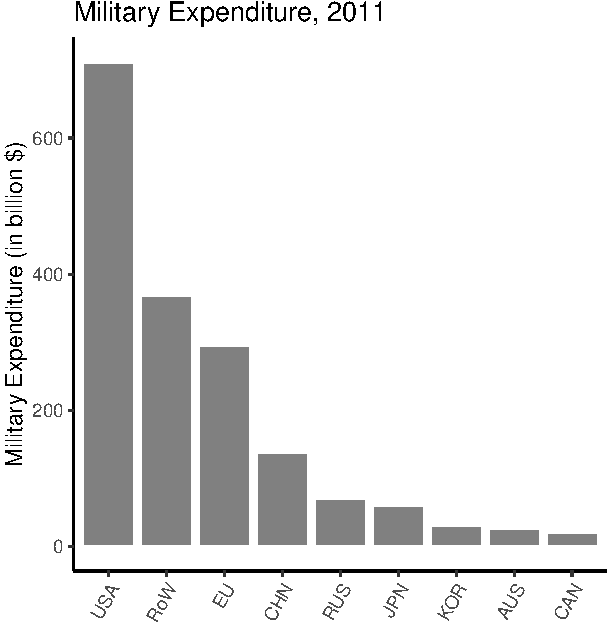
\includegraphics{figure/milex-1.pdf}
\caption{Military expenditure for in-sample governments. Values for ROW
and EU are obtained by summing expenditure of all member countries.
\label{fig:milex}}
\end{figure}

\subsection{Reduced Form Evidence on Coercion and Trade Policy}

To assist in the interpretation of the data, consider a simple bilateral
coercive bargaining setting. Governments 1 and 2 bargain over a pie of
size 1. Let \(x \in [0, 1]\) denote the share of the pie awarded to
government 1 (with the remainder, \(1-x\), going to government 2). In
the trade setting studied here, \(x=1\) might correspond to government 1
implementing optimal tariffs and government 2 liberalizing fully. Each
government's valuation of the pie is given by an increasing, weakly
concave utility function \(u_i(x)\). The value of each government's
outside option is given by a war function, \(w_i(M_i / M_j)\), which
depends on their relative military capabilities, \(\frac{M_i}{M_j}\).
Assume \(w_i\) is increasing in this military capability ratio -- that
is, more powerful governments enjoy better outside options.

For simplicity, assume the pie is divided via the Nash Bargaining
Solution, satisfying \begin{equation}
\begin{split}
x^\star \in \argmax_x & \quad \left( u_1(x) - w_1(M_1 / M_2) \right) \left( u_2(x) - w_2(M_2 / M_1) \right) \\
\text{subject to} & \quad u_1(x) \geq w_1(M_1 / M_2) \\
& \quad u_2(x) \geq w_2(M_2 / M_1) .
\end{split}
\end{equation} Taking first order conditions, it is straightforward to
show that the allocation to government 1, \(x^\star\), satisfies \[
u_1(x^\star; M_1, M_2) = \frac{u_1^\prime(x^\star)}{u_2^\prime(1 - x^\star)} \left( u_2(1 - x^\star) - w_2(M_2 / M_1) \right) + w_1(M_1 / M_2) . 
\] Differentiating this equation with respect to government 1's military
capacity, \(M_1\), we see that \(u_1(x^\star; M_1, M_2)\) is increasing
in \(M_1\), \[
\frac{\partial u_1(x^\star; M_1, M_2) }{\partial M_1} = \underbrace{- \frac{u_1^\prime(x^\star)}{u_2^\prime(1 - x^\star)} \frac{\partial w_2(M_2 / M_1)}{\partial M_1}}_{>0} + \underbrace{\frac{\partial w_1(M_1 / M_2)}{ \partial M_1}}_{>0} > 0 .
\] In other words, the distance between government 1's equilibrium
utility and the utility it receives at its ideal point is decreasing in
its relative military advantage.

Suppose that governments endeavor to maximize the welfare of the
representative consumer.\footnote{I will relax this assumption in the
  structural model developed below.} With the economy, \(h\),
calibrated, I can calculate the change in utility each representative
consumer would experience when each other government adopts free trade,
relative to their utility at the baseline set of policies. Taking this
as an empirical measure of the ratio
\(u_1(x^\star; M_1, M_2) / u_1(1)\), the model implies this quantity
will be increasing in \(M_1\), country 1's military capacity. I will
refer to this quantity as government 1's inverse \emph{conquest value}
vis-à-vis government 2.

\begin{figure}
\centering
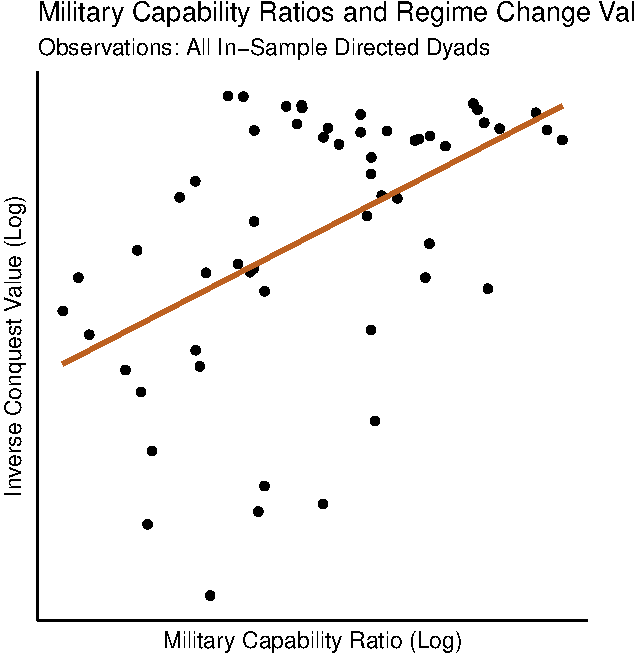
\includegraphics{figure/rcvm-1.pdf}
\caption{Correlation between military capability ratios and inverse
conquest values, all pairs of in-sample countries. \label{fig:rcvm}}
\end{figure}

Figure \ref{fig:rcvm} plots the empirical relationship between military
capability ratios and inverse conquest values. Each potential
``attacking'' country's military capability ratio vis-à-vis every
``defending'' country is plotted on the x-axis. On the y-axis is the
attacking inverse country's value for conquering each defending country.
Consistent with the predictions of this simple model, government's
inverse conquest values correlate positively with their relative
military power. Table \ref{fig:rcvm_reg_tex} and Figure
\ref{fig:rcvm_reg_dw} display the results of a series of linear models
that estimate the conditional correlations between the inverse conquest
value and the military capability ratio, distance between the countries,
and country-specific constants.

\begin{table}

\caption{\label{tab:rcvm}Inverse Conquest Values and Military Capability Ratios \label{fig:rcvm_reg_tex}}
\centering
\resizebox{\linewidth}{!}{
\begin{tabular}[t]{lllll}
\toprule
  & Base & Base (Attacker FE) & Loss of Strength & Loss of Strength (Attacker FE)\\
\midrule
Log Mil Capability Ratio & 0.016*** & 0.033*** & 0.026 & 0.045\\
 & (0.004) & (0.004) & (0.052) & (0.039)\\
Log Distance &  &  & 0.003 & 0.002\\
 &  &  & (0.010) & (0.008)\\
(Log Mil Capability Ratio) X (Log Distance) &  &  & -0.001 & -0.001\\
 &  &  & (0.006) & (0.004)\\
\midrule
Num.Obs. & 56 & 56 & 56 & 56\\
R2 & 0.247 & 0.676 & 0.249 & 0.677\\
R2 Adj. & 0.233 & 0.621 & 0.205 & 0.605\\
F & 17.720 & 12.251 & 5.739 & 9.421\\
Attacker FE? &  & ✓ &  & ✓\\
\bottomrule
\multicolumn{5}{l}{\textsuperscript{} * p < 0.1, ** p < 0.05, *** p < 0.01}\\
\end{tabular}}
\end{table}

\begin{figure}
\centering
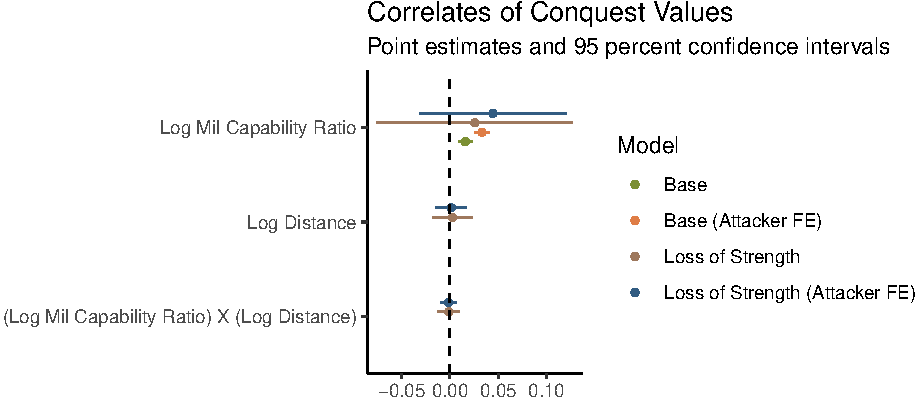
\includegraphics{figure/rcv_reg_dw-1.pdf}
\caption{Conditional correlations between inverse conquest values and
military capability ratios, geographic distance, and country-specific
constants. \label{fig:rcvm_reg_dw}}
\end{figure}

The first model confirms the statistical significance of the correlation
shown in Figure \ref{fig:rcvm}. The second model estimates this
correlation within potential ``attacking'' countries. Here, inverse
conquest values continue to rise as military advantage rises. The final
two models interact the military capability ratio with a measure of
distance between the attacker and defender. The estimated correlation
between military capability is not attenuated, but does lose statistical
significance in these specifications. Distance and the interaction of
distance with military capability does not covary with the inverse
conquest values, whether or not country-specific factors are included.
These raw correlations are informative about the role of coercion in the
formation of trade policy but suggestive at best. Trade policy
bargaining is a multilateral endeavor in which third party externalities
loom large. Moreover, governments may vary in their preferences for
protectionism, changing their ideal policies and their valuations for
conquering others. The model developed below accounts explicitly for
these features of trade policy bargaining, delivering interpretable
estimates of the effects of military capability and geographic distance
on trade policy outcomes.

\section{Model}

There are \(N\) governments, indexed
\(i \in \left\{ 1, ..., N \right\}\). Governments choose trade policies
\(\bm{\tau}_i = \left( \tau_{i1}, ..., \tau_{iN} \right) \in [1, \bar{\tau}]^N\)
which affect their welfare indirectly through changes in the
international economy.\footnote{\(\bar{\tau}\) is an arbitrarily large
  but finite value sufficient to shut down trade between any pair of
  countries.} An entry of the trade policy vector, \(\tau_{ij}\) is the
tax country \(i\) imposes on imports from \(j\).\footnote{Costs enter in
  an ``iceberg'' fashion, and I normalize \(\tau_{ii} = 1\). Then, if
  the price of a good in country \(j\) is \(p_{jj}\), its cost (less
  freight) in country \(i\) is \(\tau_{ij} p_{jj}\). The ad valorem
  tariff equivalent of the trade policy is \(t_{ij} = \tau_{ij} - 1\). I
  employ structural estimates of these costs from Cooley (2019a) to
  estimate the model, which are described in more detail in Appendix A.}
The economy, detailed in Appendix A, can be succinctly characterized by
a function \(h: \bm{\tau} \rightarrow \mathbb{R}_{++}^N\) mapping trade
policies to wages in each country, denoted
\(\bm{w} = \left( w_1, ..., w_N \right)\). These in turn determine trade
flows between pairs of countries and price levels around the
world.\footnote{The economy is a variant of the workhorse model of Eaton
  and Kortum (2002).}

Throughout, I will use \(\bm{\theta}_m\) to denote the vector of all
non-economic parameters to be estimated and \(\bm{Z}_m\) to denote the
vector of all non-economic data observed by the researcher.
\(\bm{\theta}_h\) denotes parameters associated with the economy, \(h\),
which will be calibrated. \(\bm{Z}_h\) denotes data associated with the
economy. I will explicate the elements of these vectors in the
proceeding sections and the Appendix.

Government welfare depends on the economic consequences of trade policy
choices. Governments value the welfare of a representative consumer that
resides within each country. The consumer's welfare in turn depends on
net revenues accrued through the government's trade policy distortions,
which are redistributed to the consumer. Revenues and induced welfare
can be computed given knowledge of the general equilibrium function
\(h(\bm{\tau})\). Each government's welfare is given by
\(V_i \left( h(\bm{\tau}); v_i \right)\) where \(v_i\) is a revenue
threshold parameter. This value of this function depends on the
consumer's net income and is characterized fully in the Appendix. The
consumer's net income can be written as a function of the governments'
policy choices \[
\tilde{Y}_i(h_i(\bm{\tau}))  = h_i(\bm{\tau}) L_i + r_i(h(\bm{\tau}); v_i) . 
\] \(L_i\) is the country's labor endowment, \(r_i(h(\bm{\tau}); v_i)\)
is trade policy revenues, and \(h_i(\bm{\tau})\) are equilibrium wages
in \(i\). \(v_i \in [1, \infty)\) is a structural parameter that
modulates the government's ability to extract trade policy rents.

Adjusted revenues are given by \begin{equation} \label{eq:r}
r_i(h(\bm{\tau}), v_i) = \sum_j (\tau_{ij} - v_i) X_{ij}(h(\bm{\tau}))
\end{equation} and \(X_{ij}(h(\bm{\tau}))\) are country \(i\)'s imports
from country \(j\).\footnote{This object does not correspond empirically
  to governments' factual tariff revenues, as \(\tau_{ij}\) incorporates
  a larger set of trade policy distortions than tariffs alone. Yet,
  non-tariff barriers to trade also generate rents that do not accrue
  directly to the government's accounts (see, for example, Anderson and
  Neary (1992) for the case of quotas). This revenue function is
  designed to capture this broader set of rents.} When \(v_i\) is close
to one, small policy distortions are sufficient to generate revenue for
the government. Conversely when \(v_i\) is high, the government must
erect large barriers to trade before revenues begin entering government
coffers and returning to the pockets of the consumer. Because consumers'
consumption possibilities depend on revenue generation, increasing
\(v_i\) induces governments' to become more protectionist. This
formulation provides substantial flexibility in rationalizing various
levels of protectionism, while avoiding assuming specific political
economic motivations for its genesis. From the perspective of the
consumers, rents extracted from imports are valued equally, regardless
of their source. Ex ante, governments are not discriminatory in their
trade policy preferences. Optimal policies for government \(i\) maximize
\(V_i \left( h(\bm{\tau}_i; \bm{\tau}_{-i}); v_i \right)\).

These optimal policies impose externalities on other governments. By
controlling the degree of market access afforded to foreign producers,
trade policies affect the wages of foreign workers and the welfare of
the governments that represent them. They also partially determine trade
flows, which affect other governments' ability to collect rents. In this
sense, protectionism is ``beggar thy neighbor.'' Governments' joint
policy proposals are denoted \(\tilde{\bm{\tau}}\).

Wars are fought in order to impose free trade abroad. After observing
policy proposals, governments decide whether or not to launch wars
against one another. Wars are offensive and \emph{directed}. If
government \(j\) decides to launch a war against \(i\) it pays a
dyad-specific cost, \(c_{ji}\), and imposes free trade on the target.
These war costs are modeled as realizations of a random variable from a
known family of distributions and are held as private information to the
prospective attacker. The shape of these distributions is affected by
the governments' relative power resources, denoted \(\frac{M_j}{M_i}\),
as well as the geographic distance between them, \(W_{ji}\). These
inverse value of these costs are distributed with c.d.f. \(F_{ji}\)
which is described in more detail below. I normalize the cost of
defending against aggression to zero.

If \(i\) is not attacked by any other government its announced policies
are implemented. Otherwise, free trade is imposed, setting
\(\bm{\tau}_i = \left( 1, \dots, 1 \right) = \bm{1}_i\). Substituting
these policies into \(j\)'s utility function gives
\(V_j(\bm{1}_i; \tilde{\bm{\tau}}_{-i})\) as \(j\)'s \emph{conquest
value} vis-à-vis \(i\). Note that I prohibit governments from imposing
discriminatory policies on conquered states. Substantively, this
assumption reflects the difficulty in enforcing sub-optimal policies on
prospective client states, relative to reorienting their political
institutions to favor free trade. This also ensures that the benefits of
conquest are public. However, it does not guarantee non-discrimination
in times of peace. Governments that pose the most credible threat of
conquest can extract larger policy concessions from their targets in the
form of directed trade liberalization.

Government \(j\) therefore prefers not to attack \(i\) so long as
\begin{align*}
V_j \left( \bm{1}_i; \tilde{\bm{\tau}}_{-i} \right) - c_{ji} &\leq V_j \left( \tilde{\bm{\tau}} \right) \\
c_{ji}^{-1} &\leq \left( V_j \left( \bm{1}_i; \tilde{\bm{\tau}}_{-i} \right) - V_j \left( \tilde{\bm{\tau}} \right) \right)^{-1}
\end{align*}

or if the benefits from imposing free trade on \(i\) are outweighed by
the costs, holding other governments' policies fixed. The probability
that no government finds it profitable to attack \(i\) can then be
calculated as \[
H_i \left( \tilde{\bm{\tau}}; \bm{Z}_m, \bm{\theta}_m \right) = \prod_{j \neq i} F_{ji} \left( \left( V_j \left( \bm{1}_i; \tilde{\bm{\tau}}_{-i} \right) - V_j \left( \tilde{\bm{\tau}} \right) \right)^{-1} \right)
\] I am agnostic as to the process by which the coordination problem is
resolved in the case in which multiple prospective attackers find it
profitable to attack \(i\). I assume simply that \(i\) is attacked with
certainty when it is profitable for any government to do so. This event
occurs with probability
\(1 - H_i(\tilde{\bm{\tau}}; \bm{Z}_m, \bm{\theta}_m)\).

Because of strategic interdependencies between trade policies, optimal
policy proposals are difficult to formulate. Governments face a complex
problem of forming beliefs over the probabilities that they and each of
their counterparts will face attack and the joint policies that will
result in each contingency. For simplicity, I assume governments solve
the simpler problem of maximizing their own utility, assuming no other
government faces attack. I denote this objective function with
\(G_i(\tilde{\bm{\tau}})\) which can be written
\begin{equation} \label{eq:G}
G_i(\tilde{\bm{\tau}}) = H_i(\tilde{\bm{\tau}}; \bm{Z}_m, \bm{\theta}_m) V_i(\tilde{\bm{\tau}}) + \left( 1 - H_i(\tilde{\bm{\tau}}; \bm{Z}_m, \bm{\theta}_m) \right) V_i(\bm{1}_i; \tilde{\bm{\tau}}_{-i})
\end{equation} where \(V_i(\bm{1}_i; \tilde{\bm{\tau}}_{-i})\) denotes
\(i\)'s utility when free trade is imposed upon it. This objective
function makes clear the tradeoff \(i\) faces when making policy
proposals. Policies closer to \(i\)'s ideal point deliver higher utility
conditional on peace, but raise the risk of war. Lowering barriers to
trade on threatening countries increases
\(H_i(\tilde{\bm{\tau}}; \bm{Z}, \bm{\theta}_m)\), the probability \(i\)
avoids war, at the cost of larger deviations from policy optimality.

Policy proposals are made simultaneously. Let
\(\tilde{\bm{\tau}}_i^\star(\tilde{\bm{\tau}}_{-i})\) denote a solution
to this problem and \(\tilde{\bm{\tau}}^\star\) a Nash equilibrium of
this policy announcement game.

\subsection{Policy Equilibrium in Changes}

The equilibrium of the international economy depends on a vector of
structural parameters and constants \(\bm{\theta}_h\) defined in
Appendix A. Computing the economic equilibrium
\(h(\bm{\tau}; \bm{\theta}_h)\) requires knowing these values.
Researchers have the advantage of observing data related to the
equilibrium mapping for one particular \(\bm{\tau}\), the factual trade
policies.

The estimation problem can be therefore partially ameliorated by
computing the equilibrium in \emph{changes}, relative to a factual
baseline. Consider a counterfactual trade policy \(\tau_{ij}^\prime\)
and its factual analogue \(\tau_{ij}\). The counterfactual policy can be
written in terms of a proportionate change from the factual policy with
\(\tau_{ij}^\prime = \hat{\tau}_{ij} \tau_{ij}\) where
\(\hat{\tau}_{ij} = 1\) when \(\tau_{ij}^\prime = \tau_{ij}\). By
rearranging the equilibrium conditions, I can solve the economy in
changes, replacing \(h(\bm{\tau}; \bm{\theta}_h) = \bm{w}\) with
\(\hat{h}(\hat{\bm{\tau}}; \bm{\theta}_h) = \hat{\bm{w}}\).
Counterfactual wages can then be computed as
\(\bm{w}^\prime = \bm{w} \odot \hat{\bm{w}}\).

This method is detailed in Appendix A. Because structural parameters and
unobserved constants do not change across equilibria, parameters that
enter multiplicatively drop out of the equations that define this
``hat'' equilibrium. This allows me to avoid estimating these
parameters, while enforcing that the estimated equilibrium is consistent
with their values. The methodology, introduced by Dekle, Eaton, and
Kortum (2007), is explicated further in Costinot and Rodríguez-Clare
(2015) and used to study trade policy in Ossa (2014) and Ossa (2016).

It is straightforward to extend this methodology to the game studied
here. Consider a modification to the policy-setting game described above
in which governments propose changes to factual trade policies, denoted
\(\hat{\tilde{\bm{\tau}}}\). Note that this modification is entirely
cosmetic -- the corresponding equilibrium in levels can be computed by
multiplying factual policies by the ``hat'' equilibrium values
(\(\tau_{ij}^\prime = \hat{\tau}_{ij} \tau_{ij}\)). I can then replace
the equilibrium conditions above with their analogues in changes.

Let \(\hat{V}_j(\hat{\tilde{\bm{\tau}}})\) denote changes in \(j\)'s
consumer welfare under proposed policy changes. Prospective attackers'
peace conditions can be written in changes as \[
\hat{c}_{ji}^{-1} \leq \left( \hat{V}_j \left( \bm{1}_i; \hat{\tilde{\bm{\tau}}}_{-i} \right) - \hat{V}_j \left( \hat{\tilde{\bm{\tau}}} \right) \right)^{-1}
\] where \[
\hat{c}_{ji} = \frac{c_{ji}}{V_j \left( \bm{\tau} \right)}
\] measures the share of \(j\)'s utility lost to wage a war with \(i\).
I assume the inverse relative cost of war \(j\) incurs when attacking
\(i\) is distributed Frechét with \begin{equation} \label{eq:inv_costs}
\text{Pr}\left( \frac{1}{\hat{c}_{ji}} \leq \frac{1}{\hat{c}} \right) = \hat{F}_{ji} \left( \frac{1}{\hat{c}} \right) = \exp \left( -\frac{1}{\hat{C}} \left( \frac{M_j}{M_i} \right)^{\gamma} W_{ji}^{-\alpha_1} Y_j^{\alpha_2} \hat{c}^{\eta} \right) .
\end{equation} The parameters \(\alpha_1\) and \(\gamma\) govern the
extent to which military advantage and geographic proximity are
converted into cost advantages. If \(\gamma\) is greater than zero, then
military advantage reduces the costs of war. Similarly, if \(\alpha_1\)
is greater than zero, then war costs increase with geographic distance,
consistent with a loss of strength gradient. Because costs are now
measured relative to baseline utility, I include a measure of the
attacking country's g.d.p., \(Y_j\) in the cost distribution. If
\(\alpha_2\) is positive, larger countries sacrifice a smaller
percentage of their welfare when prosecuting wars. \(\hat{C}\) and
\(\eta\) are global shape parameters that shift the cost distribution
for all potential attackers and are calibrated.\footnote{I set
  \(\hat{C}=\) 25 and \(\eta=\) 1.5. By shifting all potential
  attackers' war costs, \(\hat{C}\) modulates the probability of war in
  the data and could be estimated on data describing the likelihood of
  war between in-sample countries in any given year. Because no wars
  occur in the period I study, I do not undertake this exercise.}

Each government's objective function (\ref{eq:G}) in changes is
\begin{equation} \label{eq:Ghat}
\hat{G}_i(\hat{\tilde{\bm{\tau}}}) = \hat{H}_i(\hat{\tilde{\bm{\tau}}}; \bm{Z}, \bm{\theta}_m) \hat{V}_i(\hat{\tilde{\bm{\tau}}}) + \left( 1 - \hat{H}_i(\hat{\tilde{\bm{\tau}}}; \bm{Z}, \bm{\theta}_m) \right) \hat{V}_i(\bm{1}_i; \hat{\tilde{\bm{\tau}}}_{-i})
\end{equation} where \[
\hat{H}_i \left( \hat{\tilde{\bm{\tau}}}; \bm{Z}, \bm{\theta}_m \right) = \prod_{j \neq i} \hat{F}_{ji} \left( \left( \hat{V}_j \left( \bm{1}_i; \tilde{\bm{\tau}}_{-i} \right) - \hat{V}_j \left( \hat{\tilde{\bm{\tau}}} \right) \right)^{-1} \right) .
\] With Frechét-distributed relative costs this equation has a closed
functional form, with \[
\hat{H}_i \left( \hat{\tilde{\bm{\tau}}}; \bm{Z}, \bm{\theta}_m \right) = \exp \left( - \sum_{j \neq i} - \frac{1}{\hat{C}} \left( \frac{M_j}{M_i} \right)^{\gamma} W_{ji}^{-\alpha_1} Y_j^{\alpha_2} \left( \hat{V}_j \left( \bm{1}_i; \tilde{\bm{\tau}}_{-i} \right) - \hat{V}_j \left( \hat{\tilde{\bm{\tau}}} \right) \right)^{-\eta} \right) .
\]

Let \(\hat{\tilde{\bm{\tau}}}_i^\star(\hat{\tilde{\bm{\tau}}}_{-i})\)
denote a solution to policy change proposal problem and
\(\hat{\tilde{\bm{\tau}}}^\star(\bm{\theta}_m; \bm{Z}_m)\) a Nash
equilibrium of this policy change announcement game.

\section{Estimation}

The model's equilibrium, \(\hat{\tilde{\bm{\tau}}}^\star\) depends on a
vector of unobserved parameters
\(\bm{\theta}_m = \left( \bm{v}, \alpha_1, \alpha_2, \gamma \right)\). I
assume observed policies are generated by the model up to measurement
error \[
\tilde{\bm{\tau}} = \tilde{\bm{\tau}}^\star(\bm{\theta}_m, \bm{Z}_m) + \bm{\epsilon} . 
\] \(\bm{\epsilon}\) is an \(N \times N\) matrix with
\(\epsilon_{ii} = 0\) for all \(i\) and \(\E[\epsilon_{ij}] = 0\) for
all \(i \neq j\). Recall that \(\tilde{\bm{\tau}}^\star\) can be
reconstructed from \(\hat{\tilde{\bm{\tau}}}^\star\), the model's
equilibrium, by simply multiplying equilibrium policies by factual
policies, \(\bm{\tau}\).

Following the assumption that measurement error is mean-zero, I seek an
estimator that solves \begin{equation} \label{eq:estimator}
\min_{\bm{\theta}_m} \sum_i \sum_j \left( \epsilon_{ij}(\bm{\theta}_m, \bm{Z}_m) \right)^2 .
\end{equation}

Solving this problem presents two computational challenges. First,
computing government welfare changes for any given \(\hat{\bm{\tau}}\)
requires solving the system of equations characterizing the equilibrium
of the international economy, \(\hat{h}(\hat{\bm{\tau}})\). These
changes must be computed for both the proposed policies and for policies
imposed by each potential war. Second, computing
\(\tilde{\bm{\tau}}^\star(\bm{\theta}_m)\) requires iteratively solving
each government's best response problem until convergence at a Nash
equilibrium. I sidestep both of these by recasting the best response
problem and estimation problem as mathematical programs with equilibrium
constraints (MPECs) (Su and Judd 2012; Ossa 2014, 2016).

To reformulate the best response problem, I consider an equivalent
formulation in which each government chooses trade policies and wages,
subject to the additional constraint that chosen wages are consistent
with the general equilibrium of the international economy
(\(\hat{h}(\hat{\tilde{\bm{\tau}}}) = \hat{w}\)). Let
\(\hat{\bm{x}}_i = \left( \hat{\tilde{\bm{\tau}}}_i, \hat{\bm{w}} \right)\)
store \(i\)'s choice variables in this problem. Then, this problem can
be rewritten as follows, noting explicitly dependencies on
\(\bm{\theta}_m\) \begin{equation} \label{eq:tauTildeHatMPEC}
\begin{split}
\max_{\hat{\bm{x}}_i} & \quad \hat{G}_i(\hat{\bm{w}}; \bm{\theta}_m) \\
\text{subject to} & \quad \hat{\bm{w}} = \hat{h}(\hat{\tilde{\bm{\tau}}}) .
\end{split}
\end{equation} Let \(\mathcal{L}_i(\hat{\bm{x}}_i, \bm{\lambda}_i)\)
denote the associated Lagrangian. This formulation allows me to quickly
compute best responses
\(\hat{\tilde{\bm{\tau}}}_i(\hat{\tilde{\bm{\tau}}}_{-i})\) without
iteratively solving \(h(\hat{\tilde{\bm{\tau}}})\).

I then reformulate the estimation problem (\ref{eq:estimator}) in a
similar manner. At an interior Nash equilibrium, the gradient of the
Lagrangian is null \[
\nabla_{\hat{\tilde{\bm{\tau}}}_i} \mathcal{L}_i(\hat{\bm{x}}_i, \bm{\lambda}_i; \bm{\theta}_m) = \bm{0}
\] for each government \(i\). In the reformulated estimation problem, I
seek to choose parameters, trade policies, multipliers, and general
equilibrium response variables for the proposed policies and imposed
policies in order to minimize measurement error while enforcing these
equilibrium constraints, in addition to general equilibrium constraints.
Let
\(\hat{\bm{x}}_i^\prime = \left( \bm{1}_i, \hat{\tilde{\bm{\tau}}}_{-i}, \hat{\bm{w}}_i^\prime \right)\)
store general equilibrium equilibrium policies and wages when free trade
is imposed on \(i\).

Formally, I solve \begin{equation} \label{eq:estimatorMPEC}
\begin{split}
\min_{ \bm{\theta}_m, \hat{\tilde{\bm{\tau}}}, \hat{\bm{w}}, \hat{\bm{w}}^\prime, \bm{\lambda} } & \quad \sum_i \sum_j \left( \epsilon_{ij} \right)^2 \\
\text{subject to} & \quad \nabla_{\hat{\tilde{\bm{\tau}}}_i} \mathcal{L}_i(\hat{\bm{x}}_i, \bm{\lambda}_i; \bm{\theta}_m) = \bm{0} \text{ for all } i \\
& \quad \hat{\bm{w}} = \hat{h} \left( \hat{\tilde{\bm{\tau}}} \right) \\
& \quad \hat{\bm{w}}_i^\prime = \hat{h} \left( \bm{1}_i, \hat{\tilde{\bm{\tau}}}_{-i} \right) \text{ for all } i
\end{split}
\end{equation} The constraints collectively ensure
\(\hat{\tilde{\bm{\tau}}} = \tilde{\bm{\tau}}^\star(\bm{\theta}_m)\) --
or that the policies are consistent with Nash equilibrium in policies,
given estimated parameters.

This procedure produces point estimates \(\tilde{\bm{\theta}}_m\). I
then construct uncertainty intervals through nonparametric bootstrap,
taking 250 bootstrapped samples from the distribution of estimated
policy barriers in Cooley (2019a) and re-solving (\ref{eq:estimator}).

\section{Results}

\begin{figure}
\centering
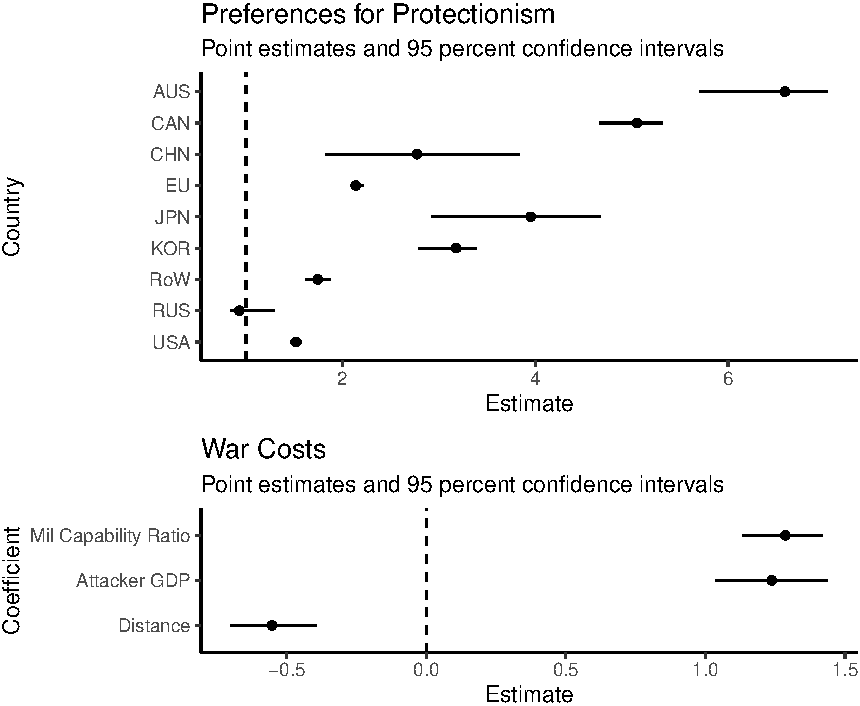
\includegraphics{figure/ests-1.pdf}
\caption{Model parameter estimates and 95 percent confidence intervals.
The top panel shows protectionism preference parameter estimates
(\(v_i\)) for each country. The bottom panel shows parameter estimates
for observables affecting costs of war (\(\gamma, \alpha_1, \alpha_2\)).
\label{fig:ests}}
\end{figure}

Figure \ref{fig:ests} displays results from the estimation. Recall that
\(v_i\) governs the ease with which governments can extract revenues
from trade policy distortions. When \(v_i\) is higher government \(i\)
prefers higher barriers to trade, all else equal. When \(v_i=1\) the
government acts as a classical social welfare maximizer. There is
considerable heterogeneity in governments' estimated preferences for
protectionism. The United States and Russia are estimated to be
relatively liberal, while Australia and Canada are quite protectionist.

An attacking country's military advantage and g.d.p. are estimated to
reduce war costs, facilitating coercion. There are increasing returns to
both of these features in reducing the average costs of war
(\(\gamma, \alpha_2 > 1\)). Economically large and military powerful
countries are the most effective at coercion, holding the distance of
their adversary constant. Figure \ref{fig:war_costs} displays estimated
average war costs, relative to those of the United States, holding the
distance to the adversary constant. Given its large economy and
military, the United States is estimated to enjoy the smallest average
war costs. The European Union, China, and Russia pay between 3 and 6
times the costs of the United States to prosecute wars on average. Wars
are estimated to cost at least an order of magnitude more than U.S. wars
for other countries in the sample.

\begin{figure}
\centering
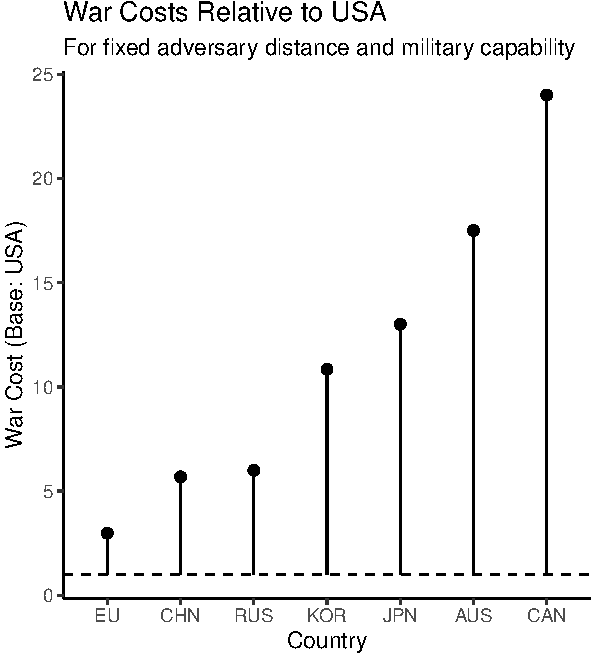
\includegraphics{figure/war_costs-1.pdf}
\caption{Estimated relative war costs against a fixed adversary. The
United States' costs serve as baseline (\(c=1\)). \label{fig:war_costs}}
\end{figure}

War costs are estimated to depend on the distance between the attacker
and potential adversary. Attackers that are more distant from their
adversaries are estimated to enjoy smaller war costs. In other words,
model estimates imply an inverse loss of strength gradient. This may
emerge due to the peculiarities of military technology in 2011, a period
in which geographic distance represents a uniquely small impediment to
the projection of force.

The model estimates can be readily transformed to deliver empirical
quantities that measure the salience of military coercion in
international relations. Figure \ref{fig:rcv} plots the estimated
conquest value for each potential attacking country vis-à-vis each
potential defending country. These quantities differ from those analyzed
in the reduced form section above in that they account explicitly for
the attacking government's preferences for protectionism. Russia's
conquest values are estimated to be among the highest in the sample.
This reflects the relatively poor market access conditions it enjoys at
the estimated equilibrium. Because their economies are the largest in
the sample, the gains that accrue from successfully conquering the
United States, China and the European Union tend to be larger than the
gains from conquering other countries. Australia, Canada, and China
benefit little from conquering others. This result obtains because of
their governments' estimated preferences for protectionism. Conquest
stimulates trade that is disadvantageous for a government \(i\) when
\(v_i\) is high and \(i\)'s trade barriers are lowered below the revenue
threshold due to the effects of coercion. This variation in conquest
values highlights the dependence of the coercive environment on the
underlying international economy and government preferences.

\begin{figure}
\centering
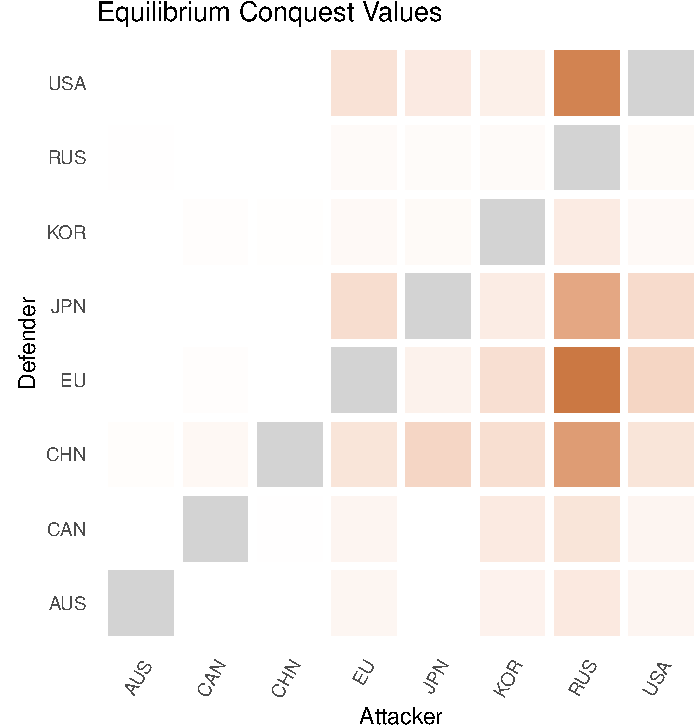
\includegraphics{figure/rcv-1.pdf}
\caption{Estimated conquest value for each potential attacking country
vis-à-vis each potential defending country. Darker colors indicate
higher conquest values. \label{fig:rcv}}
\end{figure}

It is also straightforward to calculate the equilibrium probability of
war once the model has been estimated by simply plugging parameter
estimates back into the inverse cost distribution given in Equation
\ref{eq:inv_costs}.\footnote{These estimated probabilities of war should
  be interpreted only in relative terms. The overall probability of war
  is governed by the calibrated parameter \(\hat{C}\). Higher values of
  this parameter would scale down each probability of war but would not
  shift their relative values.} Figure \ref{fig:pr_peace} plots point
estimates and uncertainty intervals surrounding the likelihood of war
between all pairs of countries in the sample. In general, governments
run very small risks of invasion from other governments. However, the
threat of war with the United States looms large in the sample. The
probabilities the United States attacks each other country in the sample
are highlighted in orange in the Figure. The European Union is also
estimated to impose substantial threats.

\begin{figure}
\centering
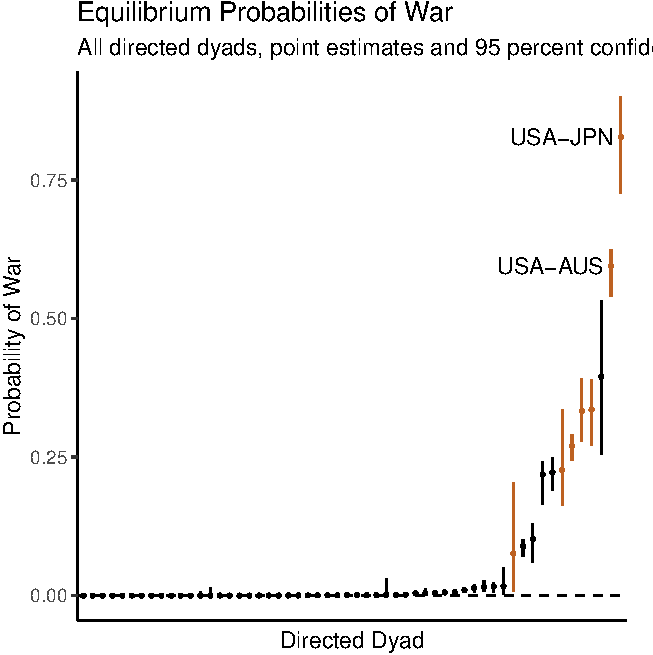
\includegraphics{figure/war_probs-1.pdf}
\caption{Estimated equilibrium probabilities of war, point estimates and
95 percent confidence intervals. Probabilities the United States attacks
each other country highlighted in orange. \label{fig:pr_peace}}
\end{figure}

It is worth noting that the countries with the highest estimated risk of
war with the United States, Japan and Australia, happen to be U.S.
allies. The security guarantees encapsulated in these alliances are not
explicitly modeled. One way to interpret these results is that
Australian and Japanese security would deteriorate rapidly in the
absence of U.S. military protection, representing an implicit threat the
United States can leverage to affect trade policy.\footnote{Lake (2007)
  would label these relationships ``hierarchical'' and based on the
  authority of the United States to dictate the policy of its
  subordinates. Still, in Lake's conceptualization, ``authority is
  buttressed by the capacity for coercion'' (p.~53).}

\subsection{Model Fit and Inferences about Policy Preferences}

\begin{figure}
\centering
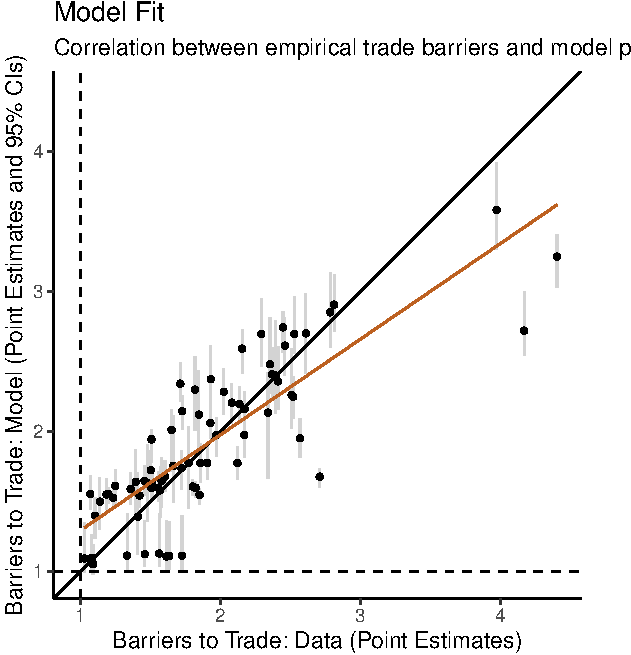
\includegraphics{figure/fit-1.pdf}
\caption{Correlation between trade barrier data and model predictions.
\label{fig:fit}}
\end{figure}

Figure \ref{fig:fit} evaluates the ability of the estimated model to
predict the level of trade barriers. The model's mean absolute error is
0.27, equivalent to a 27 percent ad valorem tariff. The model's
predictions are fairly well correlated with the trade barrier data
(\(\rho=\) 0.68). In Appendix C I plot the model's predictive error for
each directed dyad in the sample, highlighting which observations are
well explained by the model and which are not. Of note, Russia faces
uniquely poor market access conditions in the data that the model does
not fully replicate.

\begin{figure}
\centering
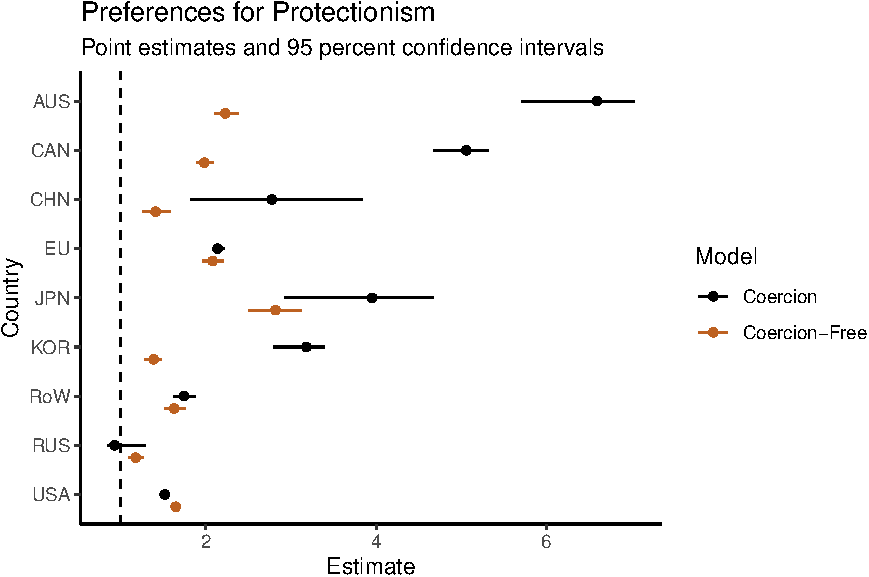
\includegraphics{figure/ests_mil_off-1.pdf}
\caption{Effect of modeling military coercion on inferences about
governments' preferences for protectionism. Figure plots point estimates
and 95 percent confidence intervals for preference parameters under
baseline model and model in which coercion is impossible.
\label{fig:ests_mil_off}}
\end{figure}

Modeling coercion explicitly both improves model fit and alters
inferences about government's underlying preferences for protectionism.
I re-estimate the model under the assumption that coercion is
impossible. In this model, equilibrium policies reflect only
governments' underlying preferences, \(v_i\). Estimated preferences for
protectionism under this model are shown in Figure
\ref{fig:ests_mil_off}. The estimated preferences of militarily powerful
countries are largely unchanged across models. This is not true for less
powerful countries. The estimated preferences of Australia, Canada, and
China move dramatically when coercion is prohibited. The model developed
here rationalizes their trade barriers as the result of highly
protectionist latent preferences tempered by the effects of
international coercion. The coercion-free model instead infers instead
that they are relatively liberal in their preferences. Leaving coercion
out of the model exerts downward bias on estimates of governments'
welfare-mindedness. A large literature employs the equilibrium trade
policies of Grossman and Helpman (1994) or Grossman and Helpman (1995)
to estimate the weight governments place on the welfare of special
interests relative to that of society at large (Goldberg and Maggi 1999;
Mitra, Thomakos, and Ulubasoglu 2006; Gawande, Krishna, and Olarreaga
2009, 2012, 2015; Ossa 2014). Because the ``protection for sale'' model
incorporates no theory of international coercion, these studies
over-estimate governments' social welfare consciousness.

Modeling coercion explicitly also improves model fit substantially. The
correlation coefficient between model predictions and observed trade
barriers falls to 0.45 when coercion is prohibited. The mean absolute
error increases 19.9 percent to 0.32. In Appendix C I replicate Figure
\ref{fig:fit} for the coercion-free model.

\section{Counterfactuals: Coercion and the World Economy}

How does the shadow of coercion affect the functioning of the world
economy? How would patterns of trade and trade protectionism change if
governments' power resources or preferences were modified? With model
estimates computed, this class of questions can be addressed through
recomputing the model's equilibrium at alternative sets of parameters or
data. In other words, compute
\(\tilde{\bm{\tau}}^\star(\bm{\theta}_m^\prime; \bm{Z}_m^\prime)\) where
\(\bm{\theta}_m^\prime\) and \(\bm{Z}_m^\prime\) are alternative
arrangements of parameters and observable model primitives,
respectively. Changes to the economy can then be computed by
substituting these counterfactual equilibrium policies into the model of
the world economy, solving
\(h \left( \tilde{\bm{\tau}}^\star(\bm{\theta}_m^\prime; \bm{Z}_m^\prime) \right)\).
I consider three counterfactual scenarios here. First, I quantify the
aggregate effects of military coercion by conducting a counterfactual in
which military coercion is prohibited. Second, I quantify the effects of
the diffusion of military power on trade policy and the international
economy by recomputing the model's equilibrium at projected levels of
military spending in 2030. Finally, I quantify the effects of
liberalizing Chinese trade policy preferences on the probability of
various wars.

\subsection{A Coercion-Free World}

First, I calculate the net economic effects of coercion by calculating
the equilibrium to a game in which coercion is impossible, holding
governments' preferences at their estimated values. The shadow of
coercion is a substantial force for trade liberalization. Moving from
this counterfactual ``pacifist'' world to the coercive equilibrium
delivers a 63 percent increase in the value of total global trade.
Figure \ref{fig:cfct1_X} disaggregates these changes in trade flows,
showing the change in imports induced by demilitarization for each
importer-exporter pair. It also shows the changes in equilibrium trade
policy that generate these changes in trade flows.

\begin{figure}
\centering
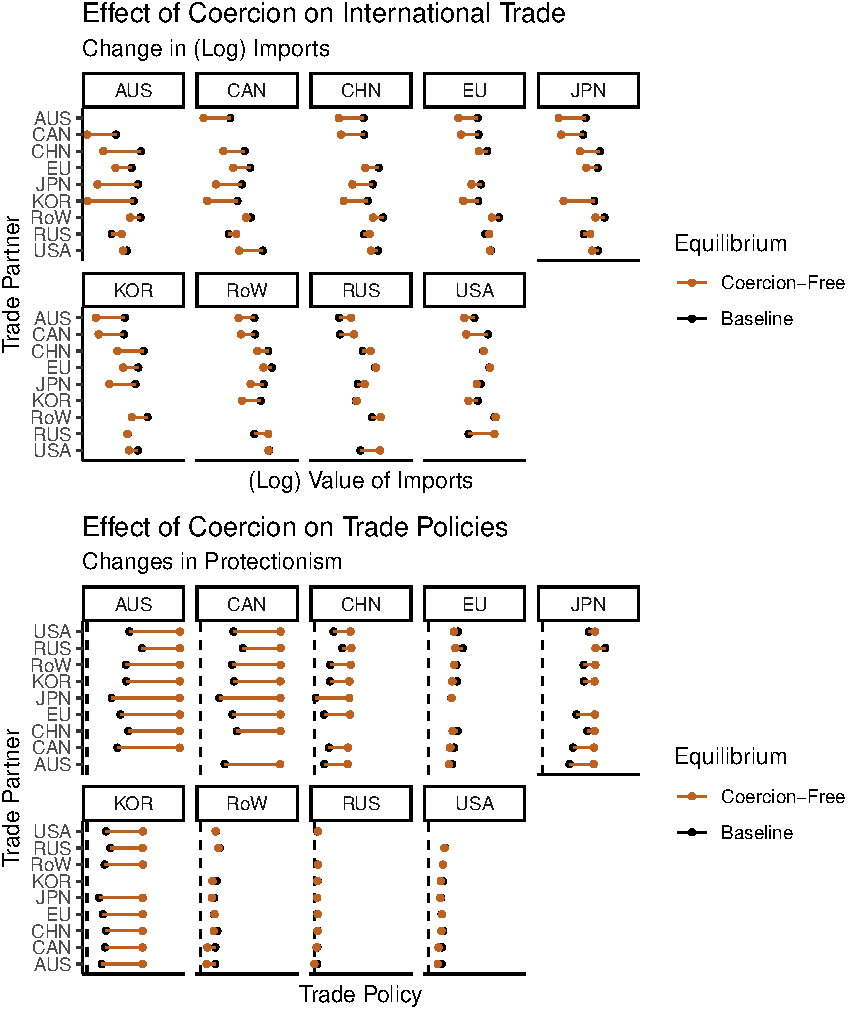
\includegraphics{figure/cfct1_X-1.pdf}
\caption{Changes in trade flows and trade policy when military coercion
is counterfactually prohibited. Top plot shows changes in the (log)
value of imports for each country in the sample, disaggregated by trade
partner. Bottom plot shows changes in equilibrium trade policies for
each country in the sample, again disaggregated by trade partner.
Counterfactual import values and trade policies are shown in orange.
\label{fig:cfct1_X}}
\end{figure}

U.S. and Russian trade policies remain largely unchanged. Yet their
trade patterns are still affected by others' changes in trade policy
behavior. Australia, Canada, China, and South Korea become substantially
more protectionist, reducing their own trade volumes and shifting
patterns of international exchange elsewhere. Trade policies in the
coercion-free world are largely homogenous within adopting countries,
reflecting the model's ex-ante incentives against policy discrimination.
The exception to this rule is for large countries like the United States
and European Union, whose counterfactual trade policies reflect
dependence on the size of their trading partners, consistent with
optimal taxation (Johnson 1953; Ossa 2014).

\begin{figure}
\centering
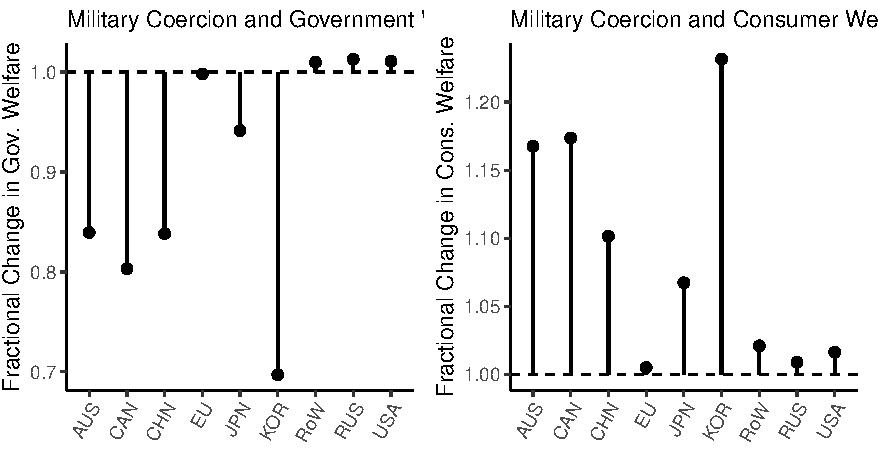
\includegraphics{figure/cfct1_welfare-1.pdf}
\caption{Changes in government welfare and consumer welfare (calculated
by setting \(v_i=1\) for all \(i\)) induced by moving from coercion-free
equilibrium to baseline equilibrium. \label{fig:cfct1_welfare}}
\end{figure}

Figure \ref{fig:cfct1_welfare} plots the changes in government and
consumer welfare due to coercion, calculated as the difference between
the coercion-free equilibrium and the baseline equilibrium. The measure
of consumer welfare is calculated by setting \(v_i=1\) for all
governments and evaluating the representative consumer's indirect
utility at equilibrium policies, consistent with the interpretation of
\(v_i\) as a political economy parameter capturing government incentives
to deviate from socially optimal trade policies. Consumers benefit
substantially from the trade liberalization induced by military
coercion, but highly protectionist governments suffer. Australia,
Canada, China, and South Korea suffer welfare losses when military
coercion is permitted, relative to the counterfactual ``pacifist''
world. The United States government gains the most from coercion among
non-RoW countries.

\subsection{Multipolarity, Trade Policy, and International Trade}

Military power in 2011 was highly concentrated in the hands of the
United States (see Figure \ref{fig:milex}). Since 2011, other countries,
China in particular, have begun to close this military capability gap
with the United States. How would the continued diffusion of military
power affect trade policy and patterns of international economic
exchange? To answer this question I project each in-sample government's
military spending in 2030, assuming military budgets grow (shrink) at
their average rate between 2011 and 2018. Projected military spending
for 2030 is shown in Figure \ref{fig:milex_2030}. The largest change is
the shift in relative military power from the United States and European
Union toward China.

\begin{figure}
\centering
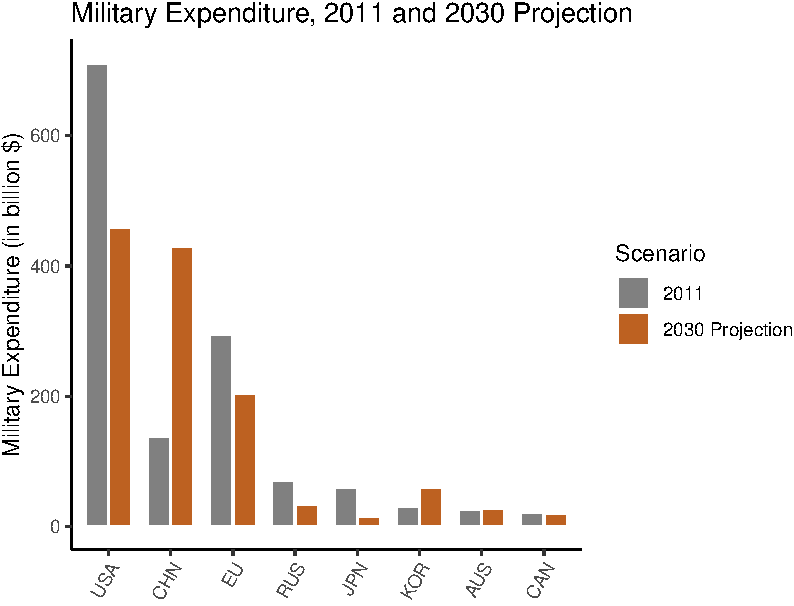
\includegraphics{figure/milex_2030-1.pdf}
\caption{Projected military spending in 2030, assuming military budgets
grow at observed average growth rate between 2011 and 2018.
\label{fig:milex_2030}}
\end{figure}

Multipolarization impacts globalization in two ways. On the one hand,
newly militarily powerful countries can resist others' demands to
liberalize, leading to a less-integrated global economy. On the other
hand, the diffusion of military power increases the coercive capacity of
some states in the system, allowing them to make greater liberalization
demands of others and contributing to global economic integration. These
effects are mediated by governments' preferences for protectionism,
which determine governments' ideal policies and the returns to coercion.
In this ``multipolarization'' scenario, China leverages these increases
in military might to adopt more restrictive trade policies. Figure
\ref{fig:cfct2_tau} displays the changes in Chinese trade policies that
result under multipolarization. On net, multipolarization is a force for
liberalization. The value of global trade under multipolarization is
110.3 percent its baseline value.

\begin{figure}
\centering
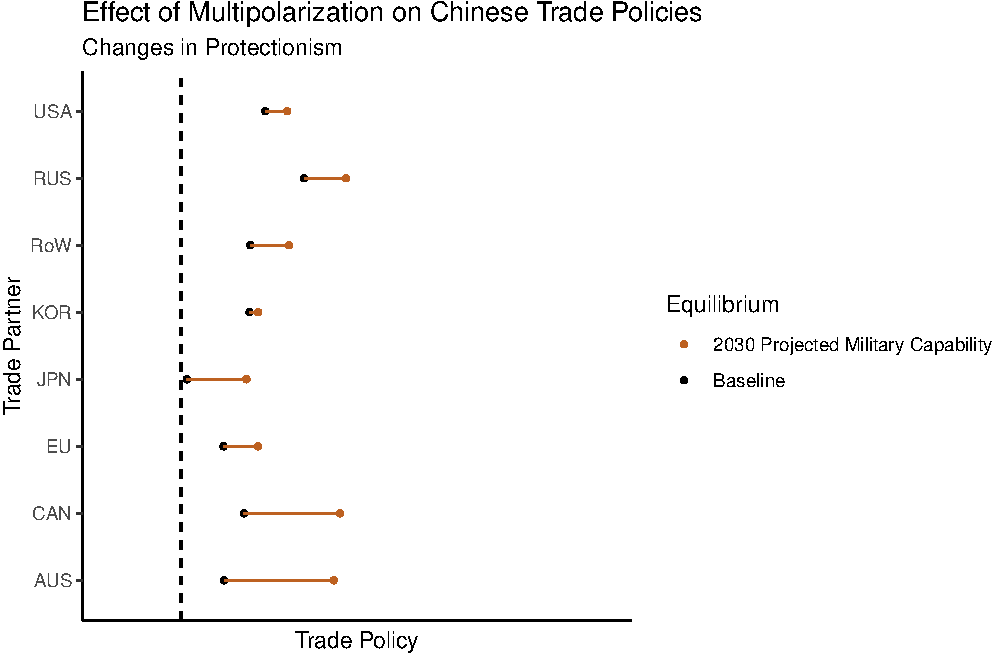
\includegraphics{figure/cfct2_tau-1.pdf}
\caption{Changes in Chinese trade policies under multipolarization.
\label{fig:cfct2_tau}}
\end{figure}

\subsection{Chinese Preference Liberalization and the Risk of War}

Reducing governments' incentives for protectionism can also decrease the
risk of war. By reducing governments incentives to adopt high trade
barriers, preference liberalization reduces others' incentives for
conquest, in turn, reducing the probability of war. To quantify these
effects, I consider a liberalization of Chinese policy preferences,
setting their revenue collection parameter to that of the United States
(\(\hat{v}_{\text{CHN}}=\) 2.77, \(v_{\text{CHN}}^\prime=\) 1.52).
Figure \ref{fig:war_probs_pp4} shows the change in the probability of
war against China that occurs as the result of this change in
preferences. The United States still poses a threat of war, but the
probability the United States launches a war against China is reduced
substantially from 33.3 percent to 5.9 percent. The probability China
faces attack from another source is virtually eliminated.

\begin{figure}
\centering
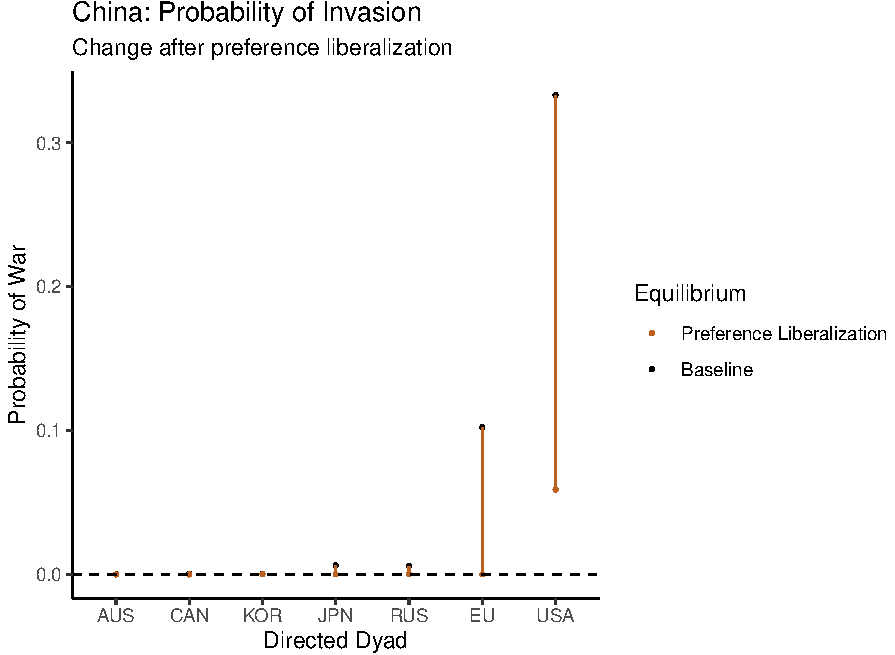
\includegraphics{figure/war_probs_pp4-1.pdf}
\caption{Changes in probability of war against China after Chinese
preference liberalization. \label{fig:war_probs_pp4}}
\end{figure}

\section{Conclusion}

The shadow of power plays a central role in international relations
theory, but measuring its effects has proved challenging. It is
axiomatic that if governments forgo war, then they must at least weakly
prefer the policy status quo to the expected policy outcomes that would
result from potential wars. In this paper, I have shown that a flexible
model of government preferences over trade outcomes can serve to
quantify government welfare under this policy counterfactual. I then
leverage the difference between factual government welfare and its
conquest values to identify parameters governing the technology of
coercion in international relations.

The preliminary estimates of these parameters suggest that military
power indeed constrains governments' policy choice in international
relations. Military spending advantage translates into battlefield
advantage. These military constraints serve to contort trade policy
toward the interests of the powerful as well as the resolved --- those
whose benefits from conquest are the largest. Military threats structure
the workings of the international economy.

Drawing these conclusions requires taking seriously extant theoretical
models of international conflict and international political economy. On
the one hand, this limits the credibility and generalizability of the
conclusions reached here --- if the models are flawed, so too will our
inferences about the world. On the other hand, this provides a
foundation upon which empirical and theoretical research in these
subfields can progress in tandem. Otherwise intractable empirical
questions can be answered, leveraging the identifying assumptions
embedded in these theories. And theories can be revised to account for
anomalous or unreasonable empirical results that rest on these
assumptions. Taking the models seriously provides answers to hard
empirical questions, along with a transparent edifice upon which those
answers rest.

\clearpage

\section{Appendix}

\subsection{A: Economy}

The economy is a variant of that of Eaton and Kortum (2002). I present
the model here for clarity, but refer interested readers to their paper
and Alvarez and Lucas (2007) for derivations and proofs of the existence
of a general equilibrium of this economy.

\subsubsection{Consumption}

Within each country resides a representative consumer which values
tradable goods and nontradable services which are aggregated in
Cobb-Douglas utility function, \(U_i\).

Consumer utility is Cobb-Douglas in a tradable goods aggregate \(Q_i\)
and non-tradable services \begin{equation} \label{eq:CD}
U_i = Q_i^{\nu_i} S_i^{1 - \nu_i}
\end{equation} \(\nu_i\) determines the consumer's relative preference
for tradables versus services. Total consumer expenditure is
\(\tilde{E}_i = E_i^q + E_i^s\) where the Cobb-Douglas preference
structure imply \(E_i^q = \nu_i \tilde{E}_i\) and
\(E_i^s = (1 - \nu_i) \tilde{E}_i\).

There is a continuum of tradable varieties indexed \(\omega \in [0,1]\)
aggregated into \(Q_i\) through a constant elasticity of substitution
function \begin{equation} \label{eq:CES}
Q_i = \left( \int_{[0,1]} q_i(\omega)^{\frac{\sigma - 1}{\sigma}} d \omega  \right)^{\frac{\sigma}{\sigma - 1}}
\end{equation} with \(\sigma > 0\). With \(E_i^q\) fixed by the
upper-level preference structure, consumers maximize \(Q_i\) subject to
their tradable budget constraint \[
\int_{[0,1]} p_i(\omega) q_i(\omega) d \omega \leq E_i^q
\] where \(p_i(\omega)\) is the price of variety \(\omega\) in country
\(i\). Let \(Q_i^\star\) denote a solution to this problem. The tradable
price index \(P_i^q\) satisfies \(P_i^q Q_i^\star = E_i^q\) with \[
P_i^q = \left( \int_{[0,1]} p_i(\omega)^{1 - \sigma} \right)^{\frac{1}{1 - \sigma}}
\]

\subsubsection{Production}

Consumers are endowed with labor \(L_i\) and earn wage \(w_i\) for
supplying labor to producers. Services are produced competitively at
cost \[
k_i^s = \frac{w_i}{z_i^s}
\] where \(z_i^s\) is country \(i\)'s productivity in services. All
countries can produce each tradable variety \(\omega\). Production
requires labor and a tradable goods bundle of intermediate inputs
(\(Q_i\)). Producing a unit of variety \(\omega\) costs \[
k_i(\omega) = \frac{1}{z_i(\omega)} w_i^{1 - \beta} \left( P_i^q \right)^\beta
\] with \(\beta \in [0,1]\) controlling the share of labor required in
production. Total expenditure on intermediates in country \(i\) is
\(E_i^x\). \(z_i(\omega)\) controls \(i\)'s productivity in producing
variety \(\omega\). \(z_i(\omega)\) is a Fréchet-distributed random
variable. \(F_i(z)\) is the probability \(i\)'s productivity in
producing a tradable variety is less than or equal to \(z\). With
\(F \sim\) Fréchet, \[
F(z) = \exp \left\{ - T_i z^{-\theta} \right\}
\] where \(T_i\) is a country-specific productivity shifter and
\(\theta > 1\) is a global parameter that controls the variance of
productivity draws around the world. When \(\theta\) is large,
productivity is less stochastic.

\subsubsection{Trade Frictions}

Let \(p_{ij}(\omega)\) denote the price in \(i\) of a variety \(\omega\)
produced in \(j\). With competitive markets in production, local prices
are equal to local costs of production, \[
p_{ii}(\omega) = k_i(\omega)
\] When shipped from \(i\) to \(j\), a variety incurs iceberg freight
costs \(\delta_{ji}\) and policy costs \(\tau_{ji}\), meaning \[
p_{ji}(\omega) = \tau_{ji} \delta_{ji} p_{ii}(\omega)
\]

Producers and consumers alike search around the world for the cheapest
variety \(\omega\), inclusive of shipping and policy costs. Equilibrium
local prices therefore satisfy \[
p_i^\star(\omega) = \min_{j \in \left\{ 1,...,N \right\}} \left\{ p_{ij} \right\}
\] The set of varieties \(i\) imports from \(j\) is \[
\Omega_{ij}^\star = \left\{ \omega \in [0,1] \left. \right\vert p_{ij}(\omega) \leq \min_{k \neq j} \left\{ p_{ik} \right\} \right\}
\]

Total expenditure in country \(i\) on goods from \(j\) (inclusive of
freight costs and policy costs) is \(X_{ij}\). At the border, the cost,
insurance, and freight (c.i.f.) value of these goods is
\(X_{ij}^{\text{cif}} = \tau_{ij}^{-1} X_{ij}\). Before shipment, their
free on board (f.o.b.) value is
\(X_{ij}^{\text{fob}} = \left( \delta_{ij} \tau_{ij} \right)^{-1} X_{ij}\)

\subsubsection{Tariff Revenue (Policy Rents)}

Governments collect the difference between each variety's final value
and its c.i.f. value. Total rents for government \(i\) are
\begin{equation} \label{eq:revenue}
r_i = \sum_j (\tau_{ij} - 1) X_{ij}^{\text{cif}}
\end{equation} This revenue is returned to the consumer, but is valued
by the government independent of its effect on the consumer's
budget.\footnote{This formulation requires the ``representative
  consumer'' to encompass individuals that have access to rents and
  those that do not. It avoids ``burning'' these rents, as would be
  implied by a model in which the government valued rents but the
  consumer did not have access to them.}

\subsubsection{Equilibrium}

In equilibrium, national accounts balance and international goods
markets clear. Total consumer expenditure is equal to the sum of labor
income, tariff revenue, and the value of trade deficits \(D_i\) \[
\tilde{E}_i = w_i L_i + r_i + D_i
\] Labor income is equal to the labor share of all sales of tradables
globally and local services sales \begin{equation} \label{eq:income}
w_i L_i = \sum_j (1 - \beta) X_{ji}^{\text{cif}} + X_i^s
\end{equation} where \[
X_i^s = E_i^s = (1 - \nu_i) (w_i L_i + r_i)
\] The remainder of consumer expenditure is spent on tradables \[
E_i^q = \nu_i (w_i L_i + r_i) + D_i
\] A \(\beta\)-fraction of producer income is spent on intermediates \[
E_i^x = \sum_j \beta X_{ji}^{\text{cif}}
\] and total tradable expenditure is \begin{equation} \label{eq:tExp}
E_i = E_i^q + E_i^x
\end{equation}

The share of \(i\)'s tradable expenditure spent on goods from \(j\) is
\begin{equation} \label{eq:shares}
x_{ij}(\bm{w}) = \frac{1}{E_i} \int_{\Omega_{ij}^\star} p_{ij}(\omega) q_i^\star \left( p_{ij} (\omega) \right) d \omega = \frac{ T_j \left( \tau_{ij} \delta_{ij} w_j^{1 - \beta} P_j^{\beta} \right)^{-\theta} }{ \frac{1}{C} \left( P_i^q(\bm{w}) \right)^{-\theta}}
\end{equation} \(q_i^\star \left( p_{ij} (\omega) \right)\) is
equilibrium consumption of variety \(\omega\) from both consumers and
producers. \(C\) is a constant function of exogenous parameters. The
tradable price index is \begin{equation} \label{eq:Pindex}
P_i^q(\bm{w}) = C \left( \sum_j T_j \left( d_{ij} w_j^{1 - \beta} P_j^{\beta} \right)^{- \theta} \right)^{-\frac{1}{\theta}}
\end{equation}

Finally, I normalize wages to be consistent with world gdp in the data.
Denoting world gdp with \(Y\), I enforce
\begin{equation} \label{eq:normalization}
Y = \sum_i w_i L_i
\end{equation}

The equilibrium of the economy depends on policy choices \(\bm{\tau}\),
trade deficits \(\bm{D}\), and a vector of structural parameters and
constants
\(\bm{\theta}_h = \left\{ L_i, T_i, \bm{\delta}, \sigma, \theta, \beta, \nu_i, \right\}_{i \in \left\{ 1, ..., N \right\}}\).

\textbf{Definition F1:} An \emph{international economic equilibrium} is
a mapping
\(h : \left\{ \bm{\tau}, \bm{D}, \bm{\theta}_h \right\} \rightarrow \mathbb{R}_{++}^N\)
with \(h(\bm{\tau}, \bm{D}; \bm{\theta}_h) = \bm{w}\) solving the system
of equations given by \ref{eq:revenue}, \ref{eq:income}, \ref{eq:tExp},
\ref{eq:shares}, \ref{eq:Pindex}, and \ref{eq:normalization}.

Alvarez and Lucas (2007) demonstrate the existence and uniqueness of
such an equilibrium, subject to some restrictions on the values of
structural parameters and the magnitude of trade costs.

\subsubsection{Welfare}

With the equilibrium mapping in hand, I can connect trade policies to
government welfare given in Equation \ref{eq:G}. Consumer indirect
utility is \begin{equation} \label{eq:V}
V_i(\bm{w}) = \frac{\tilde{E}_i(\bm{w})}{P_i(\bm{w})}
\end{equation} where \(P_i\) is the aggregate price index in country
\(i\) and can be written \[
P_i(\bm{w}) = \left( \frac{P_i^q(\bm{w})}{\nu_i} \right)^{\nu_i} \left( \frac{P_i^s(\bm{w})}{1 - \nu_i} \right)^{1 - \nu_i}
\] \(P_i^q\) is given in equation \ref{eq:Pindex} and
\(P_i^s = \frac{w_i}{A_i}\). Substituting \(\bm{w}\) with its
equilibrium value \(h(\bm{\tau}, \bm{D}; \bm{\theta}_h)\) returns
consumer indirect utility as a function of trade policies. Equilibrium
trade flows can be computed as \[
X_{ij}^{\text{cif}}(\bm{w}) = \tau_{ij}^{-1} x_{ij}(\bm{w}) E_i(\bm{w})
\] Substituting these into the revenue equation (\ref{eq:revenue}) gives
the revenue component of the government's objective function.

\subsubsection{Equilibrium in Changes}

In ``hats,'' the equilibrium conditions corresponding to
\ref{eq:revenue}, \ref{eq:income}, \ref{eq:tExp}, \ref{eq:shares},
\ref{eq:Pindex}, and \ref{eq:normalization} are
\begin{equation} \label{eq:revenueHat}
\hat{r}_i = \frac{1}{r_i} \left( E_i \hat{E}_i(\hat{\bm{w}}) - \sum_j X_{ij}^{\text{cif}} \hat{X}_{ij}^{\text{cif}}(\hat{\bm{w}}) \right)
\end{equation} \begin{equation} \label{eq:incomeHat}
\hat{w}_i = \frac{1}{\nu_i w_i L_i} \left( \sum_j \left( (1 - \beta) X_{ji}^{\text{cif}} \hat{X}_{ji}^{\text{cif}}(\hat{\bm{w}}) \right) + (1 - \nu_i) r_i \hat{r}_i(\hat{\bm{w}}) \right)
\end{equation} \begin{equation} \label{eq:tExpHat}
\hat{E}_i(\hat{\bm{w}}) = \frac{1}{E_i} \left( E_i^q \hat{E}_i^q(\hat{\bm{w}}) + E_i^x \hat{E}_i^x(\hat{\bm{w}}) \right)
\end{equation} \begin{equation} \label{eq:sharesHat}
\hat{x}_{ij}(\hat{\bm{w}}) = \left( \hat{\tau}_{ij} \hat{w}_j^{1 - \beta} \hat{P}_j(\hat{\bm{w}})^\beta \right)^{-\theta} \hat{P}_i(\hat{\bm{w}})^{\theta}
\end{equation} \begin{equation} \label{eq:PindexHat}
\hat{P}_i(\hat{\bm{w}}) = \left( \sum_j x_{ij} \left( \hat{\tau}_{ij} \hat{w}_j^{1 - \beta} \hat{P}_j(\hat{\bm{w}})^\beta \right)^{-\theta} \right)^{-\frac{1}{\theta}}
\end{equation} \begin{equation} \label{eq:normalizationHat}
1 = \sum_i y_i \hat{w}_i
\end{equation} where \[
y_i = \frac{w_i L_i}{\sum_j w_j L_j}
\]

This transformation reduces the vector of parameters to be calibrated to
\(\bm{\theta}_h = \left\{\theta, \beta, \nu_i, \right\}_{i \in \left\{ 1, ..., N \right\}}\).

\textbf{Definition A2:} An \emph{international economic equilibrium in
changes} is a mapping
\(\hat{h} : \left\{ \hat{\bm{\tau}}, \hat{\bm{D}}, \bm{\theta}_h \right\} \rightarrow \mathbb{R}_{++}^N\)
with
\(\hat{h}(\hat{\bm{\tau}}, \hat{\bm{D}}; \bm{\theta}_h) = \hat{\bm{w}}\)
solving the system of equations given by \ref{eq:revenueHat},
\ref{eq:incomeHat}, \ref{eq:tExpHat}, \ref{eq:sharesHat},
\ref{eq:PindexHat}, and \ref{eq:normalizationHat}.

\subsubsection{Welfare in Changes}

Now changes in consumer welfare can be calculated for any set of trade
policy changes \(\hat{\bm{\tau}}\). Manipulating \ref{eq:V}, changes in
consumer indirect utility are \begin{equation} \label{eq:VHat}
\hat{V}_i(\bm{w}) = \frac{\hat{\tilde{E}}_i(\hat{\bm{w}})}{\hat{P}_i(\hat{\bm{w}})}
\end{equation} where \[
\hat{P}_i(\hat{\bm{w}}) = \hat{P}_i^q(\hat{\bm{w}})^{\nu_i} \hat{P}_i^s(\hat{\bm{w}})^{\nu_i - 1}
\] and \(\hat{P}_i^q(\hat{\bm{w}})\) is given by equation
\ref{eq:PindexHat} and \(\hat{P}_i^s(\hat{\bm{w}}) = \hat{w}_i\).
Changes in policy rents are given by equation \ref{eq:revenueHat}.

\subsection{B: Calibration of Economy}

Solving for an international equilibrium in changes (Definition A2)
requires data on national accounts (\(E_i\), \(E_i^q\), \(E_i^x\),
\(w_i L_i\)), and international trade flows (\(X_{ij}^{\text{cif}}\))
(collectively, \(\bm{Z}_h\)), the magnitude of observed policy barriers
to trade (\(\tau_{ij}\)), and the structural parameters \(\theta\),
\(\beta\), and \(\bm{\nu}\) (collectively, \(\bm{\theta}_h\)). Policy
barriers are estimated using the methodology developed in Cooley
(2019a). To maintain consistency with the model developed there, I
employ the same data on the subset of countries analyzed here. I refer
readers to that paper for a deeper discussion of these choices, and
briefly summarize the calibration of the economy here.

\subsubsection{Data}

Trade flows valued pre-shipment (free on board) are available from
\href{https://comtrade.un.org/db/default.aspx}{COMTRADE}. I employ
cleaned data from
\href{http://www.cepii.fr/CEPII/en/welcome.asp}{CEPII}'s
\href{http://www.cepii.fr/cepii/en/bdd_modele/presentation.asp?id=1}{BACI}.
To get trade in c.i.f. values, I add estimated freight costs from Cooley
(2019a) to these values. Total home expenditure (\(X_{ii} + X_i^s\)) and
aggregate trade imbalances \(D_i\) can then be inferred from national
accounts data (GDP, gross output, and gross consumption). GDP gives
\(w_i L_i\) and gross consumption gives \(E_i^s + E_i^q + X_i^x\). To
isolate expenditure on services, I use data from the World Bank's
International Comparison Program, which reports consumer expenditure
shares on various good categories. I classify these as tradable and
nontradable, and take the sum over expenditure shares on tradables as
the empirical analogue to \(\nu_i\). Then, expenditure on services is
\(X_i^s = (1 - \nu_i) w_i L_i\).

\subsubsection{Structural Parameters}

I set \(\theta =\) 6, in line with estimates reported in Head and Mayer
(2014) and Simonovska and Waugh (2014). A natural empirical analogue for
\(\beta\) is intermediate imports \((E_i - w_i L_i)\) divided by total
tradable production. This varies country to country, however, and
equilibrium existence requires a common \(\beta\). I therefore take the
average of this quantity as the value for \(\beta\), which is 0.86 in my
data. This means that small changes around the factual equilibrium
result in discontinuous jumps in counterfactual predictions. I therefore
first generate counterfactual predictions with this common \(\beta\),
and use these as a baseline for analysis.

\subsubsection{Trade Imbalances}

As noted by Ossa (2014), the assumption of exogenous and fixed trade
imbalances generates implausible counterfactual predictions when trade
frictions get large. I therefore first purge aggregate deficits from the
data, solving \(\hat{h}(\hat{\bm{\tau}}, \bm{0}; \bm{\theta}_h)\),
replicating Dekle, Eaton, and Kortum (2007). This counterfactual,
deficit-less economy is then employed as the baseline, where
\(\hat{h}(\hat{\bm{\tau}}; \bm{\theta}_h)\) referring to a
counterfactual prediction from this baseline.

\subsubsection{Trade Barrier Estimates}

\begin{figure}
\centering
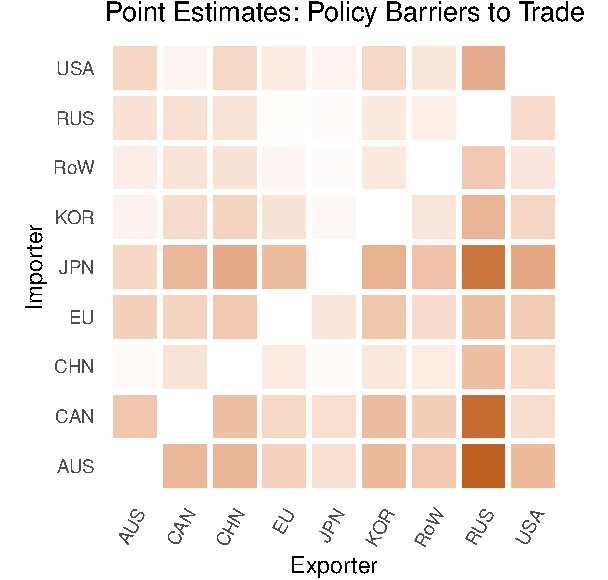
\includegraphics{figure/tauhm-1.pdf}
\caption{Distribution of policy barriers to trade. Each cell reports the
magnitude of the policy barrier each importing country (y-axis) imposes
on every exporting country (x-axis). \label{fig:tauhm}}
\end{figure}

\subsection{C: Other Measures of Model Fit}

\begin{figure}
\centering
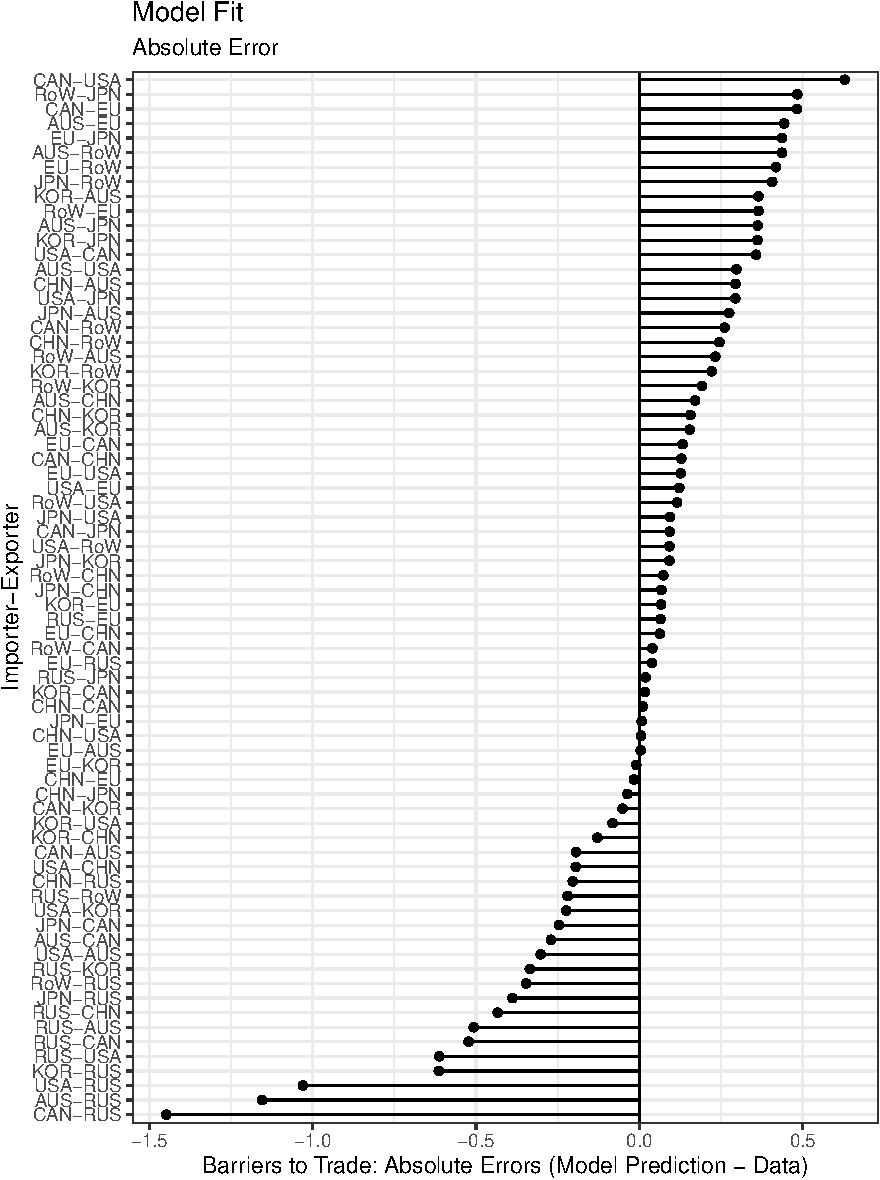
\includegraphics{figure/fit_ddyad-1.pdf}
\caption{Absolute errors for each directed dyad in the sample. Positive
values indicate that the model predicts a higher trade barrier than is
observed in the data (point estimate). \label{fig:fit_ddyad}}
\end{figure}

\begin{figure}
\centering
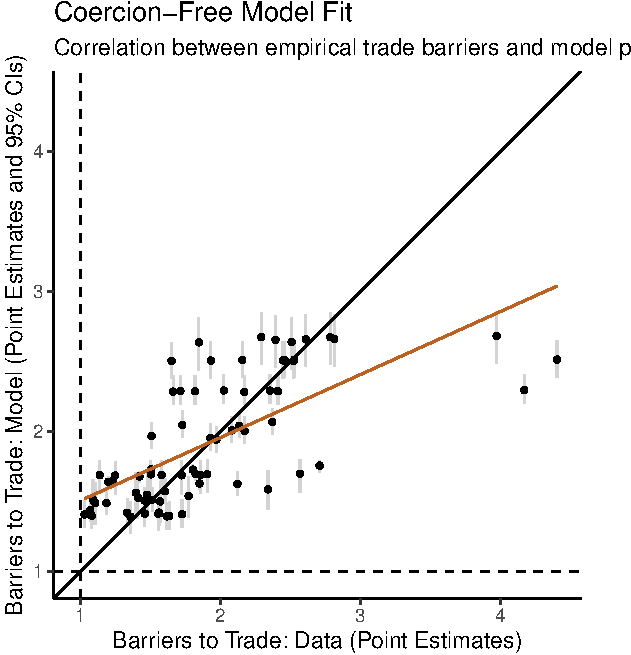
\includegraphics{figure/fit_mo-1.pdf}
\caption{Correlation between trade barrier data and coercion-free model
predictions. \label{fig:fit_mo}}
\end{figure}

\clearpage

\clearpage

\chapter*{Software}

\addcontentsline{toc}{chapter}{Software}

\sloppy

Arel-Bundock V (2018). \emph{countrycode: Convert Country Names and
Country Codes}. R package version 1.1.0, \textless URL:
https://CRAN.R-project.org/package=countrycode\textgreater.

Arel-Bundock V (2020). \emph{countrycode: Convert Country Names and
Country Codes}. R package version 1.2.0, \textless URL:
https://CRAN.R-project.org/package=countrycode\textgreater.

Arel-Bundock V (2020). \emph{modelsummary: Summary Tables and Plots for
Statistical Models and Data: Beautiful, Customizable, and
Publication-Ready}. R package version 0.6.0.9000, \textless URL:
https://vincentarelbundock.github.io/modelsummary/\textgreater.

Arel-Bundock V, Enevoldsen N, Yetman C (2018). ``countrycode: An R
package to convert country names and country codes.'' \emph{Journal of
Open Source Software}, \emph{3}(28), 848. \textless URL:
https://doi.org/10.21105/joss.00848\textgreater.

Arnold JB (2019). \emph{ggthemes: Extra Themes, Scales and Geoms for
`ggplot2'}. R package version 4.2.0, \textless URL:
https://CRAN.R-project.org/package=ggthemes\textgreater.

Bache SM, Wickham H (2014). \emph{magrittr: A Forward-Pipe Operator for
R}. R package version 1.5, \textless URL:
https://CRAN.R-project.org/package=magrittr\textgreater.

Boettiger C (2020). \emph{knitcitations: Citations for `Knitr' Markdown
Files}. R package version 1.0.10, \textless URL:
https://github.com/cboettig/knitcitations\textgreater.

Boettiger C (2019). \emph{knitcitations: Citations for `Knitr' Markdown
Files}. R package version 1.0.10, \textless URL:
https://CRAN.R-project.org/package=knitcitations\textgreater.

Chang W, Wickham H (2019). \emph{ggvis: Interactive Grammar of
Graphics}. R package version 0.4.5, \textless URL:
https://CRAN.R-project.org/package=ggvis\textgreater.

Cooper N (2018). \emph{NCmisc: Miscellaneous Functions for Creating
Adaptive Functions and Scripts}. R package version 1.1.6, \textless URL:
https://CRAN.R-project.org/package=NCmisc\textgreater.

Cooper N (2017). \emph{reader: Suite of Functions to Flexibly Read Data
from Files}. R package version 1.0.6, \textless URL:
https://CRAN.R-project.org/package=reader\textgreater.

Francois R (2020). \emph{bibtex: Bibtex Parser}. R package version
0.4.2.2, \textless URL:
https://CRAN.R-project.org/package=bibtex\textgreater.

from mda:mars SMD, utilities with Thomas Lumley's RTUAMF (2019).
\emph{earth: Multivariate Adaptive Regression Splines}. R package
version 5.1.2, \textless URL:
https://CRAN.R-project.org/package=earth\textgreater.

Gloeckner N (2020). \emph{olpsR: Algorithms and functions for On-line
Portfolio Selection}. R package version 0.5.

Henry L, Wickham H (2019). \emph{purrr: Functional Programming Tools}. R
package version 0.3.3, \textless URL:
https://CRAN.R-project.org/package=purrr\textgreater.

Henry L, Wickham H (2020). \emph{purrr: Functional Programming Tools}. R
package version 0.3.4, \textless URL:
https://CRAN.R-project.org/package=purrr\textgreater.

Hlavac M (2018). \emph{stargazer: Well-Formatted Regression and Summary
Statistics Tables}. R package version 5.2.2, \textless URL:
https://CRAN.R-project.org/package=stargazer\textgreater.

Hornik K, Feinerer I, Kober M (2017). \emph{skmeans: Spherical k-Means
Clustering}. R package version 0.2-11, \textless URL:
https://CRAN.R-project.org/package=skmeans\textgreater.

Kassambara A (2019). \emph{ggpubr: `ggplot2' Based Publication Ready
Plots}. R package version 0.2.4, \textless URL:
https://CRAN.R-project.org/package=ggpubr\textgreater.

Kassambara A (2020). \emph{ggpubr: `ggplot2' Based Publication Ready
Plots}. R package version 0.4.0, \textless URL:
https://CRAN.R-project.org/package=ggpubr\textgreater.

Lemon J, Bolker B, Oom S, Klein E, Rowlingson B, Wickham H, Tyagi A,
Eterradossi O, Grothendieck G, Toews M, Kane J, Turner R, Witthoft C,
Stander J, Petzoldt T, Duursma R, Biancotto E, Levy O, Dutang C, Solymos
P, Engelmann R, Hecker M, Steinbeck F, Borchers H, Singmann H, Toal T,
Ogle D, Baral D, Groemping U, Venables B (2019). \emph{plotrix: Various
Plotting Functions}. R package version 3.7-7, \textless URL:
https://CRAN.R-project.org/package=plotrix\textgreater.

Meschiari S (2015). \emph{latex2exp: Use LaTeX Expressions in Plots}. R
package version 0.4.0, \textless URL:
https://CRAN.R-project.org/package=latex2exp\textgreater.

Milborrow S (2019). \emph{plotmo: Plot a Model's Residuals, Response,
and Partial Dependence Plots}. R package version 3.5.6, \textless URL:
https://CRAN.R-project.org/package=plotmo\textgreater.

Müller K, Wickham H (2020). \emph{tibble: Simple Data Frames}. R package
version 3.0.1, \textless URL:
https://CRAN.R-project.org/package=tibble\textgreater.

Müller K, Wickham H (2020). \emph{tibble: Simple Data Frames}. R package
version 3.0.3, \textless URL:
https://CRAN.R-project.org/package=tibble\textgreater.

Oliphant TE (2006). \emph{A guide to NumPy}, volume 1. Trelgol
Publishing USA.

Ooms J (2020). \emph{magick: Advanced Graphics and Image-Processing in
R}. R package version 2.4.0, \textless URL:
https://CRAN.R-project.org/package=magick\textgreater.

Pedersen TL (2019). \emph{patchwork: The Composer of ggplots}. R package
version 0.0.1.9000, \textless URL:
https://github.com/thomasp85/patchwork\textgreater.

Pedersen TL (2020). \emph{patchwork: The Composer of Plots}. R package
version 1.0.1, \textless URL:
https://CRAN.R-project.org/package=patchwork\textgreater.

R Core Team (2019). \emph{R: A Language and Environment for Statistical
Computing}. R Foundation for Statistical Computing, Vienna, Austria.
\textless URL: https://www.R-project.org/\textgreater.

R Core Team (2020). \emph{R: A Language and Environment for Statistical
Computing}. R Foundation for Statistical Computing, Vienna, Austria.
\textless URL: https://www.R-project.org/\textgreater.

Ram K, Yochum C (2020). \emph{rdrop2: Programmatic Interface to the
`Dropbox' API}. R package version 0.8.2.1, \textless URL:
https://CRAN.R-project.org/package=rdrop2\textgreater.

Ripley B (2016). \emph{nnet: Feed-Forward Neural Networks and
Multinomial Log-Linear Models}. R package version 7.3-12, \textless URL:
https://CRAN.R-project.org/package=nnet\textgreater.

Robinson D, Hayes A, Couch S (2020). \emph{broom: Convert Statistical
Objects into Tidy Tibbles}. R package version 0.7.0, \textless URL:
https://CRAN.R-project.org/package=broom\textgreater.

Sievert C, Parmer C, Hocking T, Chamberlain S, Ram K, Corvellec M,
Despouy P (2020). \emph{plotly: Create Interactive Web Graphics via
`plotly.js'}. R package version 4.9.2.1, \textless URL:
https://CRAN.R-project.org/package=plotly\textgreater.

Slowikowski K (2019). \emph{ggrepel: Automatically Position
Non-Overlapping Text Labels with `ggplot2'}. R package version 0.8.1,
\textless URL: https://CRAN.R-project.org/package=ggrepel\textgreater.

Slowikowski K (2020). \emph{ggrepel: Automatically Position
Non-Overlapping Text Labels with `ggplot2'}. R package version 0.8.2,
\textless URL: https://CRAN.R-project.org/package=ggrepel\textgreater.

Snow G (2016). \emph{TeachingDemos: Demonstrations for Teaching and
Learning}. R package version 2.10, \textless URL:
https://CRAN.R-project.org/package=TeachingDemos\textgreater.

Solt F, Hu Y (2018). \emph{dotwhisker: Dot-and-Whisker Plots of
Regression Results}. R package version 0.5.0, \textless URL:
https://CRAN.R-project.org/package=dotwhisker\textgreater.

Thoen E (2020). \emph{padr: Quickly Get Datetime Data Ready for
Analysis}. R package version 0.5.2, \textless URL:
https://CRAN.R-project.org/package=padr\textgreater.

Ushey K, Allaire J, Tang Y (2020). \emph{reticulate: Interface to
`Python'}. R package version 1.16, \textless URL:
https://CRAN.R-project.org/package=reticulate\textgreater.

Van Rossum G, Drake FL (2009). \emph{Python 3 Reference Manual}.
CreateSpace, Scotts Valley, CA. ISBN 1441412697.

Virtanen P, Gommers R, Oliphant TE, Haberland M, Reddy T, Cournapeau D,
Burovski E, Peterson P, Weckesser W, Bright J, van der Walt SJ, Brett M,
Wilson J, Jarrod Millman K, Mayorov N, Nelson AR, Jones E, Kern R,
Larson E, Carey C, Polat İ, Feng Y, Moore EW, Vand erPlas J, Laxalde D,
Perktold J, Cimrman R, Henriksen I, Quintero E, Harris CR, Archibald AM,
Ribeiro AH, Pedregosa F, van Mulbregt P, Contributors S10 (2020).
``SciPy 1.0: Fundamental Algorithms for Scientific Computing in
Python.'' \emph{Nature Methods}. doi: 10.1038/s41592-019-0686-2 (URL:
https://doi.org/10.1038/s41592-019-0686-2).

Wächter A, Biegler LT (2006). ``On the implementation of an
interior-point filter line-search algorithm for large-scale nonlinear
programming.'' \emph{Mathematical Programming}, \emph{106}(1), 25-57.

Wickham H (2019). \emph{forcats: Tools for Working with Categorical
Variables (Factors)}. R package version 0.4.0, \textless URL:
https://CRAN.R-project.org/package=forcats\textgreater.

Wickham H (2017). \emph{reshape2: Flexibly Reshape Data: A Reboot of the
Reshape Package}. R package version 1.4.3, \textless URL:
https://CRAN.R-project.org/package=reshape2\textgreater.

Wickham H (2019). \emph{stringr: Simple, Consistent Wrappers for Common
String Operations}. R package version 1.4.0, \textless URL:
https://CRAN.R-project.org/package=stringr\textgreater.

Wickham H (2017). \emph{tidyverse: Easily Install and Load the
`Tidyverse'}. R package version 1.2.1, \textless URL:
https://CRAN.R-project.org/package=tidyverse\textgreater.

Wickham H (2020). \emph{forcats: Tools for Working with Categorical
Variables (Factors)}. R package version 0.5.0, \textless URL:
https://CRAN.R-project.org/package=forcats\textgreater.

Wickham H (2020). \emph{reshape2: Flexibly Reshape Data: A Reboot of the
Reshape Package}. R package version 1.4.4, \textless URL:
https://CRAN.R-project.org/package=reshape2\textgreater.

Wickham H (2020). \emph{tidyr: Tidy Messy Data}. R package version
1.1.2, \textless URL:
https://CRAN.R-project.org/package=tidyr\textgreater.

Wickham H (2019). \emph{tidyverse: Easily Install and Load the
`Tidyverse'}. R package version 1.3.0, \textless URL:
https://CRAN.R-project.org/package=tidyverse\textgreater.

Wickham H (2016). \emph{ggplot2: Elegant Graphics for Data Analysis}.
Springer-Verlag New York. ISBN 978-3-319-24277-4, \textless URL:
https://ggplot2.tidyverse.org\textgreater.

Wickham H (2007). ``Reshaping Data with the reshape Package.''
\emph{Journal of Statistical Software}, \emph{21}(12), 1-20.
\textless URL: http://www.jstatsoft.org/v21/i12/\textgreater.

Wickham H, Averick M, Bryan J, Chang W, McGowan LD, François R,
Grolemund G, Hayes A, Henry L, Hester J, Kuhn M, Pedersen TL, Miller E,
Bache SM, Müller K, Ooms J, Robinson D, Seidel DP, Spinu V, Takahashi K,
Vaughan D, Wilke C, Woo K, Yutani H (2019). ``Welcome to the
tidyverse.'' \emph{Journal of Open Source Software}, \emph{4}(43), 1686.
doi: 10.21105/joss.01686 (URL: https://doi.org/10.21105/joss.01686).

Wickham H, Bryan J (2019). \emph{readxl: Read Excel Files}. R package
version 1.3.1, \textless URL:
https://CRAN.R-project.org/package=readxl\textgreater.

Wickham H, Chang W, Henry L, Pedersen TL, Takahashi K, Wilke C, Woo K,
Yutani H, Dunnington D (2020). \emph{ggplot2: Create Elegant Data
Visualisations Using the Grammar of Graphics}. R package version 3.3.0,
\textless URL: https://CRAN.R-project.org/package=ggplot2\textgreater.

Wickham H, Chang W, Henry L, Pedersen TL, Takahashi K, Wilke C, Woo K,
Yutani H, Dunnington D (2020). \emph{ggplot2: Create Elegant Data
Visualisations Using the Grammar of Graphics}. R package version 3.3.2,
\textless URL: https://CRAN.R-project.org/package=ggplot2\textgreater.

Wickham H, François R, Henry L, Müller K (2020). \emph{dplyr: A Grammar
of Data Manipulation}. R package version 1.0.2, \textless URL:
https://CRAN.R-project.org/package=dplyr\textgreater.

Wickham H, François R, Henry L, Müller K (2020). \emph{dplyr: A Grammar
of Data Manipulation}. R package version 0.8.5, \textless URL:
https://CRAN.R-project.org/package=dplyr\textgreater.

Wickham H, Henry L (2019). \emph{tidyr: Tidy Messy Data}. R package
version 1.0.0, \textless URL:
https://CRAN.R-project.org/package=tidyr\textgreater.

Wickham H, Hester J, Francois R (2018). \emph{readr: Read Rectangular
Text Data}. R package version 1.3.1, \textless URL:
https://CRAN.R-project.org/package=readr\textgreater.

Wilke CO (2018). \emph{ggridges: Ridgeline Plots in `ggplot2'}. R
package version 0.5.1, \textless URL:
https://CRAN.R-project.org/package=ggridges\textgreater.

Xiao N (2018). \emph{ggsci: Scientific Journal and Sci-Fi Themed Color
Palettes for `ggplot2'}. R package version 2.9, \textless URL:
https://CRAN.R-project.org/package=ggsci\textgreater.

Xie Y (2019). \emph{knitr: A General-Purpose Package for Dynamic Report
Generation in R}. R package version 1.25, \textless URL:
https://CRAN.R-project.org/package=knitr\textgreater.

Xie Y (2020). \emph{knitr: A General-Purpose Package for Dynamic Report
Generation in R}. R package version 1.29, \textless URL:
https://CRAN.R-project.org/package=knitr\textgreater.

Xie Y (2015). \emph{Dynamic Documents with R and knitr}, 2nd edition.
Chapman and Hall/CRC, Boca Raton, Florida. ISBN 978-1498716963,
\textless URL: https://yihui.org/knitr/\textgreater.

Xie Y (2014). ``knitr: A Comprehensive Tool for Reproducible Research in
R.'' In Stodden V, Leisch F, Peng RD (eds.), \emph{Implementing
Reproducible Computational Research}. Chapman and Hall/CRC. ISBN
978-1466561595, \textless URL:
http://www.crcpress.com/product/isbn/9781466561595\textgreater.

Zeileis A, Croissant Y (2018). \emph{Formula: Extended Model Formulas}.
R package version 1.2-3, \textless URL:
https://CRAN.R-project.org/package=Formula\textgreater.

Zhu H (2019). \emph{kableExtra: Construct Complex Table with `kable' and
Pipe Syntax}. R package version 1.1.0, \textless URL:
https://CRAN.R-project.org/package=kableExtra\textgreater.

Zhu H (2020). \emph{kableExtra: Construct Complex Table with `kable' and
Pipe Syntax}. R package version 1.2.1, \textless URL:
https://CRAN.R-project.org/package=kableExtra\textgreater.

\chapter*{References}

\addcontentsline{toc}{chapter}{References}
\bibliographystyle{plain}
\bibliography{bib/library.bib}

\hypertarget{refs}{}
\begin{cslreferences}
\leavevmode\hypertarget{ref-Acemoglu2005b}{}%
Acemoglu, Daron. 2005. ``Politics and economics in weak and strong
states.'' \emph{Journal of Monetary Economics} 52 (7): 1199--1226.

\leavevmode\hypertarget{ref-Adao2017}{}%
Adao, Rodrigo, Arnaud Costinot, and Dave Donaldson. 2017.
``Nonparametric Counterfactual Predictions in Neoclassical Models of
International Trade.'' \emph{American Economic Review} 107 (3): 633--89.

\leavevmode\hypertarget{ref-Aghion2007}{}%
Aghion, Philippe, Pol Antràs, and Elhanan Helpman. 2007. ``Negotiating
free trade.'' \emph{Journal of International Economics} 73: 1--30.

\leavevmode\hypertarget{ref-Alvarez2007}{}%
Alvarez, Fernando, and Robert E Lucas. 2007. ``General equilibrium
analysis of the Eaton--Kortum model of international trade.''
\emph{Journal of Monetary Economics} 54: 1726--68.

\leavevmode\hypertarget{ref-Markowitz2020}{}%
Anders, Therese, Christopher J Fariss, and Jonathan N Markowitz. 2020.
``Bread Before Guns or Butter: Introducing Surplus Domestic Product
(SDP).'' \emph{International Studies Quarterly} 64: 392--405.

\leavevmode\hypertarget{ref-Anderson1996}{}%
Anderson, James E, and J. Peter Neary. 1996. ``A New Approach to
Evaluating Trade Policy.'' \emph{The Review of Economic Studies} 63 (1):
107.

\leavevmode\hypertarget{ref-Anderson1992}{}%
Anderson, James E, and J Peter Neary. 1992. ``Trade Reform with Quotas,
Partial Rent Retention, and Tariffs.'' \emph{Econometrica} 60 (1):
57--76.

\leavevmode\hypertarget{ref-Anderson2003}{}%
Anderson, James E, and Eric Van Wincoop. 2003. ``Gravity with Gravitas:
A Solution to the Border Puzzle.'' \emph{The American Economic Review}
93 (1): 170--92.

\leavevmode\hypertarget{ref-Anderson2004}{}%
---------. 2004. ``Trade Costs.'' \emph{Journal of Economic Literature}
42: 691--751.

\leavevmode\hypertarget{ref-Anderson2005}{}%
Anderson, Kym, and Will Martin. 2005. \emph{Agricultural Trade Reform
and the Doha Development Agenda}. The World Bank.

\leavevmode\hypertarget{ref-Angell1911}{}%
Angell, Norman. 1911. \emph{The great illusion: a study of the relation
of military power in nations to their economic and social advantage}.
McClelland; Goodchild.

\leavevmode\hypertarget{ref-Antras2011}{}%
Antràs, Pol, and Gerard Padró i Miquel. 2011. ``Foreign influence and
welfare.'' \emph{Journal of International Economics} 84 (2): 135--48.

\leavevmode\hypertarget{ref-Arkolakis2012}{}%
Arkolakis, Costas, Arnaud Costinot, and Andrés Rodriguez-Clare. 2012.
``New trade models, same old gains?'' \emph{The American Economic
Review} 102 (1): 94--130.

\leavevmode\hypertarget{ref-Art1996}{}%
Art, Robert J. 1996. ``American foreign policy and the fungibility of
force.'' \emph{Security Studies} 5 (4): 7--42.

\leavevmode\hypertarget{ref-Autor2013}{}%
Autor, David H, David Dorn, and Gordon H Hanson. 2013. ``The China
syndrome: Local labor market effects of import competition in the United
States.'' \emph{The American Economic Review} 103 (6): 2121--68.

\leavevmode\hypertarget{ref-Baccini2019}{}%
Baccini, Leonardo. 2019. ``The Economics and Politics of Preferential
Trade Agreements.'' \emph{Annual Review of Political Science} 22.

\leavevmode\hypertarget{ref-Baggs2005}{}%
Baggs, Jen. 2005. ``Firm survival and exit in response to trade
liberalization.'' \emph{Canadian Journal of Economics} 38 (4): 1364--83.

\leavevmode\hypertarget{ref-Bagwell1999}{}%
Bagwell, Kyle, and Robert W. Staiger. 1999. ``An economic theory of
GATT.'' \emph{American Economic Review} 89 (1): 215--48.

\leavevmode\hypertarget{ref-Bagwell2004}{}%
Bagwell, Kyle, and Robert W Staiger. 2004. \emph{The economics of the
world trading system}. MIT Press.

\leavevmode\hypertarget{ref-Bagwell2018b}{}%
Bagwell, Kyle, Robert W Staiger, and Ali Yurukoglu. 2018a.
``"Nash-in-Nash" Tariff Bargaining with and without MFN.''

\leavevmode\hypertarget{ref-Bagwell2018a}{}%
---------. 2018b. ``Quantitative Analysis of Multi-Party Tariff
Negotiations.''

\leavevmode\hypertarget{ref-Baldwin2016}{}%
Baldwin, Richard. 2016. ``The World Trade Organization and the Future of
Multilateralism.'' \emph{Journal of Economic Perspectives} 30: 95--116.

\leavevmode\hypertarget{ref-Barari2019}{}%
Barari, Soubhik, In Song Kim, and Weihuang Wong. 2019. ``Trade
Liberalization and Regime Type: Evidence from a New Tariff-line
Dataset.''

\leavevmode\hypertarget{ref-Barbieri2009}{}%
Barbieri, Katherine, Omar M. G. Keshk, and Brian M Pollins. 2009.
``Trading Data: Evaluating our Assumptions and Coding Rules.''
\emph{Conflict Management and Peace Science} 26 (5): 471--91.

\leavevmode\hypertarget{ref-Barbieri2008}{}%
Barbieri, Katherine, Omar Keshk, and Brian M Pollins. 2008. ``Correlates
of war project trade data set codebook, Version 4.0.''
\url{http://correlatesofwar.org/}.

\leavevmode\hypertarget{ref-Barbieri1999}{}%
Barbieri, Katherine, and Jack S Levy. 1999. ``Sleeping with the enemy:
The impact of war on trade.'' \emph{Journal of Peace Research} 36 (4):
463--79.

\leavevmode\hypertarget{ref-Beckley2010}{}%
Beckley, Michael. 2010. ``Economic Development and Military
Effectiveness.'' \emph{The Journal of Strategic Studies} 33 (1): 43--79.

\leavevmode\hypertarget{ref-Beckley2018}{}%
---------. 2018. ``The Power of Nations: Measuring What Matters.''
\emph{International Security} 43 (2): 7--44.

\leavevmode\hypertarget{ref-Behrens2011}{}%
Behrens, Kristian, and Pierre M. Picard. 2011. ``Transportation, freight
rates, and economic geography.'' \emph{Journal of International
Economics} 85 (2): 280--91.

\leavevmode\hypertarget{ref-Benson2007}{}%
Benson, Brett V, and Emerson M S Niou. 2007. ``Economic Interdependence
and Peace: A Game-Theoretic Analysis.'' \emph{Journal of East Asian
Studies} 7 (1): 35--59.

\leavevmode\hypertarget{ref-Berger2013}{}%
Berger, Daniel, William Easterly, Nathan Nunn, and Shanker Satyanath.
2013. ``Commercial imperialism? Political influence and trade during the
Cold War.'' \emph{The American Economic Review} 103 (2): 863--96.

\leavevmode\hypertarget{ref-Bergstrand2013}{}%
Bergstrand, Jeffrey H., Peter Egger, and Mario Larch. 2013. ``Gravity
Redux: Estimation of gravity-equation coefficients, elasticities of
substitution, and general equilibrium comparative statics under
asymmetric bilateral trade costs.'' \emph{Journal of International
Economics} 89 (1): 110--21.

\leavevmode\hypertarget{ref-Bertoli2016}{}%
Bertoli, Simone, Michaël Goujon, and Olivier Santoni. 2016. ``The
CERDI-seadistance database.'' CERDI.

\leavevmode\hypertarget{ref-Betz2017}{}%
Betz, Timm. 2017. ``Trading Interests: Domestic Institutions,
International Negotiations, and the Politics of Trade.'' \emph{Journal
of Politics} 79 (4).

\leavevmode\hypertarget{ref-Betz2019}{}%
Betz, Timm, and Amy Pond. 2019. ``The Absence of Consumer Interests in
Trade Policy.'' \emph{Journal of Politics}.

\leavevmode\hypertarget{ref-Bils2017}{}%
Bils, Peter, and William Spaniel. 2017. ``Policy bargaining and
militarized conflict.'' \emph{Journal of Theoretical Politics} 29 (4):
647--78.

\leavevmode\hypertarget{ref-Bolt2018}{}%
Bolt, Jutta, Robert Inklaar, Herman de Jong, and Jan Luiten van Zanden.
2018. ``Rebasing `Maddison': new income comparisons and the shape of
long-run economic development.'' \emph{GGDC Research Memorandum} 174.

\leavevmode\hypertarget{ref-Boulding1962}{}%
Boulding, Kenneth E. 1962. ``Conflict and defense: A general theory.''

\leavevmode\hypertarget{ref-Bove2014}{}%
Bove, Vincenzo, Leandro Elia, and Petros G. Sekeris. 2014. ``US Security
Strategy and the Gains from Bilateral Trade.'' \emph{Review of
International Economics} 22 (5): 863--85.

\leavevmode\hypertarget{ref-Bradford2003}{}%
Bradford, Scott. 2003. ``Paying the Price: Final Goods Protection in
OECD Countries.'' \emph{Review of Economics and Statistics} 85 (1):
24--37.

\leavevmode\hypertarget{ref-Brancaccio2020}{}%
Brancaccio, Giulia, Myrto Kalouptsidi, and Theodore Papageorgiou. 2020.
``Geography, Transportation, and Endogenous Trade Costs.''
\emph{Econometrica} 88 (2): 657--91.

\leavevmode\hypertarget{ref-Brito1985}{}%
Brito, Dagobert L., and Michael D. Intrilagator. 1985. ``Conflict, War,
and Redistribution.'' \emph{American Political Science Review} 79 (4).

\leavevmode\hypertarget{ref-Broda2008}{}%
Broda, Christian, Nuno Limao, and David. E. Weinstein. 2008. ``Optimal
Tariffs and Market Power: The Evidence.'' \emph{American Economic
Review} 98 (5): 2032--65.

\leavevmode\hypertarget{ref-BuenodeMesquita1980}{}%
Bruce Bueno de Mesquita. 1980. ``An Expected Utility Theory of
International Conflict.'' \emph{The American Political Science Review}
74 (4): 917--31.

\leavevmode\hypertarget{ref-BuenodeMesquita2003}{}%
Bueno De Mesquita, Bruce, Alastair Smith, Randolph M Siverson, and James
D Morrow. 2003. \emph{The logic of political survival}. MIT press.

\leavevmode\hypertarget{ref-Burgess2010}{}%
Burgess, Robin, and Dave Donaldson. 2010. ``Can Openness Mitigate the
Effects of Weather Shocks? Evidence from India's Famine Era.''
\emph{American Economic Review: Papers \& Proceedings} 100: 449--53.

\leavevmode\hypertarget{ref-Caliendo2019}{}%
Caliendo, Lorenzo, Maximiliano Dvorkin, and Fernando Parro. 2019.
``Trade and Labor Market Dynamics: General Equilibrium Analysis of the
China Trade Shock.'' \emph{Econometrica} 87 (3): 741--835.

\leavevmode\hypertarget{ref-Carnegie2014}{}%
Carnegie, Allison. 2014. ``States Held Hostage: Political Hold-Up
Problems and the Effects of International Institutions.'' \emph{American
Political Science Review} 108 (01): 54--70.

\leavevmode\hypertarget{ref-Carroll2018}{}%
Carroll, Robert J. 2018. ``War and Peace in the Marketplace.''

\leavevmode\hypertarget{ref-Carroll2019}{}%
Carroll, Robert J, and Brenton Kenkel. 2019. ``Prediction, Proxies, and
Power.'' \emph{American Journal of Political Science} 63 (3): 577--93.

\leavevmode\hypertarget{ref-Caselli2015}{}%
Caselli, Francesco, Massimo Morelli, and Dominic Rohner. 2015. ``The
Geography of Interstate Resource Wars.'' \emph{The Quarterly Journal of
Economics} 130 (1): 267--315.

\leavevmode\hypertarget{ref-Chaney2008}{}%
Chaney, Thomas. 2008. ``Distorted Gravity: The Intensive and Extensive
Margins of International Trade.'' \emph{American Economic Review} 98
(4): 1707--21.

\leavevmode\hypertarget{ref-Chapman2015}{}%
Chapman, Terrence L., Patrick J McDonald, and Scott Moser. 2015. ``The
Domestic Politics of Strategic Retrenchment, Power Shifts, and
Preventive War.'' \emph{International Studies Quarterly} 59 (1):
133--44.

\leavevmode\hypertarget{ref-Chatagnier2015}{}%
Chatagnier, J Tyson, and Kerim Can Kavakli. 2015. ``From Economic
Competition to Military Combat: Export Similarity and International
Conflict.'' \emph{Journal of Conflict Resolution}, 1--27.

\leavevmode\hypertarget{ref-Coe2011}{}%
Coe, Andrew J. 2011. ``Costly Peace: A New Rationalist Explanation for
War.''

\leavevmode\hypertarget{ref-CoeND}{}%
---------. n.d. ``The Modern Economic Peace.''

\leavevmode\hypertarget{ref-Comerford2015}{}%
Comerford, David, and José V Rodríguez Mora. 2015. ``The Gains from
Economic Integration.''

\leavevmode\hypertarget{ref-Cooley2019b}{}%
Cooley, Brendan. 2019a. ``Estimating Policy Barriers to Trade.''

\leavevmode\hypertarget{ref-Cooley2019a}{}%
---------. 2019b. ``Gunboat Diplomacy: Political Bias, Trade Policy, and
War.''

\leavevmode\hypertarget{ref-Costinot2015}{}%
Costinot, Arnaud, and Andrés Rodríguez-Clare. 2015. ``Trade Theory with
Numbers: Quantifying the Consequences of Globalization.'' \emph{Handbook
of International Economics} 4: 197--261.

\leavevmode\hypertarget{ref-Dahl1957}{}%
Dahl, Robert A. 1957. ``The Concept of Power.'' \emph{Behavioral
Science} 2 (3): 201--15.

\leavevmode\hypertarget{ref-Davis2006}{}%
Davis, Christina L. 2006. ``Do WTO Rules Create a Level Playing Field
for Developing Countries?'' In \emph{Negotiating Trade: Developing
Countries in the Wto and Nafta}. Cambridge, UK: Cambridge University
Press.

\leavevmode\hypertarget{ref-Deaton2010}{}%
Deaton, Angus, and Alan Heston. 2010. ``Understanding PPPs and PPP-based
National Accounts.'' \emph{American Economic Journal: Macroeconomics} 2
(4): 1--35.

\leavevmode\hypertarget{ref-Dekle2007}{}%
Dekle, Robert, Jonathan Eaton, and Samuel Kortum. 2007. ``Unbalanced
trade.'' \emph{AEA Papers and Proceedings} 97 (2): 351--55.

\leavevmode\hypertarget{ref-deSousa2012}{}%
De Sousa, José, Thierry Mayer, and Soledad Zignago. 2012. ``Market
access in global and regional trade.'' \emph{Regional Science and Urban
Economics}.

\leavevmode\hypertarget{ref-Diehl1985}{}%
Diehl, Paul F. 1985. ``Continuity and Military Escalation in Major Power
Rivalries, 1816-1980.'' \emph{The Journal of Politics} 47 (4): 1203--11.

\leavevmode\hypertarget{ref-Dixit1977}{}%
Dixit, Avinash, and Joseph E Stiglitz. 1977. ``Monopolistic Competition
and Optimum Product Diversity.'' \emph{The American Economic Review} 67
(3): 297--308.

\leavevmode\hypertarget{ref-Dollar2004}{}%
Dollar, David, and Aart Kraay. 2004. ``Trade, Growth, and Poverty.''
\emph{The Economic Journal} 114 (493): F22--F49.

\leavevmode\hypertarget{ref-Drezner2013}{}%
Drezner, Daniel W. 2013. ``Military Primacy Doesn't Pay (Nearly As Much
As You Think).'' \emph{International Security} 38 (2): 52--79.

\leavevmode\hypertarget{ref-Dube2011}{}%
Dube, Arindrajit, Ethan Kaplan, and Suresh Naidu. 2011. ``Coups,
Corporations, and Classified Information.'' \emph{Quarterly Journal of
Economics} 126: 1375--1409.

\leavevmode\hypertarget{ref-Dur2014}{}%
Dür, Andreas, Leonardo Baccini, and Manfred Elsig. 2014. ``The design of
international trade agreements: Introducing a new dataset.''
\emph{Review of International Organizations} 9: 353--75.

\leavevmode\hypertarget{ref-Eaton2002}{}%
Eaton, Jonathan, and Samuel Kortum. 2002. ``Technology, geography, and
trade.'' \emph{Econometrica} 70 (5): 1741--79.

\leavevmode\hypertarget{ref-Evenett2004}{}%
Evenett, Simon J., and Bernard Hoekman. 2004. \emph{Government
Procurement: Market Access, Transparency, and Multilateral Trade Rules}.
Policy Research Working Papers. The World Bank.

\leavevmode\hypertarget{ref-Fajgelbaum2016}{}%
Fajgelbaum, Pablo D, and Amit K Khandelwal. 2016. ``Measuring the
Unequal Gains from Trade.'' \emph{Quarterly Journal of Economics},
1113--80.

\leavevmode\hypertarget{ref-Fearon1995}{}%
Fearon, James D. 1995. ``Rationalist explanations for war.''
\emph{International Organization} 49 (03): 379--414.

\leavevmode\hypertarget{ref-Fearon1997}{}%
---------. 1997. ``Signaling foreign policy interests: Tying hands
versus sinking costs.'' \emph{Journal of Conflict Resolution} 41 (1):
68--90.

\leavevmode\hypertarget{ref-Fey2019}{}%
Fey, Mark, and Brenton Kenkel. 2019. ``Is an Ultimatum the Last Word on
Crisis Bargaining?'' \emph{Journal of Politics}.

\leavevmode\hypertarget{ref-Findlay2007}{}%
Findlay, Ronald., and Kevin H. O'Rourke. 2007. \emph{Power and plenty :
trade, war, and the world economy in the second millennium}. Princeton
University Press.

\leavevmode\hypertarget{ref-Fordham1998}{}%
Fordham, Benjamin O. 1998. ``Economic Interests, Party, and Ideology in
Early Cold War Era U.S. Foreign Policy.'' \emph{International
Organization} 52 (2): 359--96.

\leavevmode\hypertarget{ref-Fordham2019}{}%
---------. 2019. ``The Domestic Politics of World Power: Explaining
Debates over the United States Battleship Fleet, 1890-91.''
\emph{International Organization}, 1--34.

\leavevmode\hypertarget{ref-Fordham2005}{}%
Fordham, Benjamin O, and Thomas C Walker. 2005. ``Kantian Liberalism,
Regime Type, and Military Resource Allocation: Do Democracies Spend
Less?'' \emph{International Studies Quarterly} 49 (1): 141--57.

\leavevmode\hypertarget{ref-Gallagher1953}{}%
Gallagher, John, and Ronald Robinson. 1953. ``The Imperialism of Free
Trade.'' \emph{The Economic History Review} 6 (1): 1--15.

\leavevmode\hypertarget{ref-Garfinkel2011}{}%
Garfinkel, Michelle R, Stergios Skaperdas, and Constantinos Syropoulos.
2011. ``Trade in the Shadow of Power.''

\leavevmode\hypertarget{ref-Gartzke2011}{}%
Gartzke, Erik, and Alex Braithwaite. 2011. ``Power, Parity and
Proximity.''

\leavevmode\hypertarget{ref-Gartzke2015}{}%
Gartzke, Erik, and Jiakun Jack Zhang. 2015. ``Trade and War.'' In
\emph{The Oxford Handbook of the Political Economy of International
Trade}, edited by Lisa L Martin. Oxford University Press.

\leavevmode\hypertarget{ref-Gawande1999}{}%
Gawande, Kishore, and Wendy L. Hansen. 1999. ``Retaliation, Bargaining,
and the Pursuit of "Free and Fair" Trade.'' \emph{International
Organization} 53 (1): 117--59.

\leavevmode\hypertarget{ref-Gawande2009}{}%
Gawande, Kishore, Pravin Krishna, and Marcelo Olarreaga. 2009. ``What
governments maximize and why: the view from trade.'' \emph{International
Organization} 63 (03): 491--532.

\leavevmode\hypertarget{ref-Gawande2015}{}%
---------. 2015. ``A Political-Economic Account of Global Tariffs.''
\emph{Economics \& Politics} 27 (2): 204--33.

\leavevmode\hypertarget{ref-Gawande2012}{}%
---------. 2012. ``Lobbying Competition over Trade Policy.''
\emph{International Economic Review} 53 (1): 115--32.

\leavevmode\hypertarget{ref-Gerschenkron1943}{}%
Gerschenkron, Alexander. 1943. \emph{Bread and Democracy in Germany}.
Cornell University Press.

\leavevmode\hypertarget{ref-Gibler2014}{}%
Gibler, Douglas M, and Jaroslav Tir. 2014. ``Territorial Peace and
Democratic Clustering.'' \emph{Journal of Politics} 76 (1): 27--40.

\leavevmode\hypertarget{ref-Gilpin1981}{}%
Gilpin, Robert. 1981. \emph{War and change in world politics}. Cambridge
University Press.

\leavevmode\hypertarget{ref-Goldberg1999}{}%
Goldberg, Pinelopi Koujianou, and Giovanni Maggi. 1999. ``Protection for
Sale: An Empirical Investigation.'' \emph{American Economic Review},
1135--55.

\leavevmode\hypertarget{ref-Goldberg2016}{}%
Goldberg, P K, and N Pavcnik. 2016. ``The Effects of Trade Policy.''
\emph{Handbook of Commercial Policy} 1: 161--206.

\leavevmode\hypertarget{ref-Gowa1993}{}%
Gowa, Joanne, and Edward D Mansfield. 1993. ``Power Politics and
International Trade.'' \emph{The American Political Science Review} 87
(2): 408--20.

\leavevmode\hypertarget{ref-Grossman1994}{}%
Grossman, Gene M, and Elhanan Helpman. 1994. ``Protection for Sale.''
\emph{The American Economic Review}, 833--50.

\leavevmode\hypertarget{ref-Grossman1995}{}%
---------. 1995. ``Trade Wars and Trade Talks.'' \emph{Journal of
Political Economy}, 675--708.

\leavevmode\hypertarget{ref-Grossman1996}{}%
---------. 1996. ``Electoral Competition and Special Interest
Politics.'' \emph{Review of Economic Studies} 63: 265--86.

\leavevmode\hypertarget{ref-Grossman2016}{}%
Grossman, G. M. 2016. ``The Purpose of Trade Agreements.'' In
\emph{Handbook of Commercial Policy}, 380--434.

\leavevmode\hypertarget{ref-Guisinger2009}{}%
Guisinger, Alexandra. 2009. ``Determining Trade Policy: Do Voters Hold
Politicians Accountable?'' \emph{International Organization} 63 (3):
533--57.

\leavevmode\hypertarget{ref-Gulotty2020}{}%
Gulotty, Robert. 2020. \emph{Narrowing the Channel: The Politics of
Regulatory Protection in International Trade}. University of Chicago
Press.

\leavevmode\hypertarget{ref-Head2014}{}%
Head, Keith, and Thierry Mayer. 2014. ``Gravity Equations: Workhorse,
Toolkit and Cookbook.'' In \emph{Handbook of International Economics},
edited by Elhanan Helpman, G. Gopinath, and K. Rogoff, 4th ed., 131--96.

\leavevmode\hypertarget{ref-Head2010}{}%
Head, Keith, Thierry Mayer, and John Ries. 2010. ``The erosion of
colonial trade linkages after independence.'' \emph{Journal of
International Economics} 81: 1--14.

\leavevmode\hypertarget{ref-Head2001}{}%
Head, Keith, and John Ries. 2001. ``Increasing Returns Versus National
Product Differentiation as an Explanation for the Pattern of U.S.-Canada
Trade.'' \emph{American Economic Review} 91 (4).

\leavevmode\hypertarget{ref-Helpman2008}{}%
Helpman, Elhanan, Marc Melitz, and Yona Rubinstein. 2008. ``Estimating
Trade Flows: Trading Partners and Trading Volumes.'' \emph{Quarterly
Journal of Economics} 123 (2): 441--87.

\leavevmode\hypertarget{ref-Hirschman1945}{}%
Hirschman, Albert O. 1945. \emph{National power and the structure of
foreign trade}. Univ of California Press.

\leavevmode\hypertarget{ref-Hiscox2002}{}%
Hiscox, Michael J, and Scott L Kastner. 2002. ``A General Measure of
Trade Policy Orientations: Gravity-Model-Based Estimates for 82 Nations,
1960 to 1992.''

\leavevmode\hypertarget{ref-Ikenberry2011}{}%
Ikenberry, G John. 2011. \emph{Liberal Leviathan: The Origins, Crisis,
and Transformation of the American World Order}. Princeton, NJ:
Princeton University Press.

\leavevmode\hypertarget{ref-Jackson2007}{}%
Jackson, Matthew O, and Massimo Morelli. 2007. ``Political bias and
war.'' \emph{The American Economic Review}, 1353--73.

\leavevmode\hypertarget{ref-Jackson2009}{}%
---------. 2009a. ``Strategic Militarization, Deterrence and Wars.''
\emph{Quarterly Journal of Political Science} 4: 279--313.

\leavevmode\hypertarget{ref-Jackson2009b}{}%
---------. 2009b. ``The Reasons for Wars - An Updated Survey.'' In
\emph{Handbook on the Political Economy of War}, edited by Chris Coyne.
Elgar Publishing.

\leavevmode\hypertarget{ref-Johnson1953}{}%
Johnson, Harry G. 1953. ``Optimum tariffs and retaliation.'' \emph{The
Review of Economic Studies} 21 (2): 142--53.

\leavevmode\hypertarget{ref-Kadera2004}{}%
Kadera, Kelly, and Gerald L Sorokin. 2004. ``Measuring National Power,
International Interactions.'' \emph{International Interactions} 30 (3):
211--30.

\leavevmode\hypertarget{ref-Kee2009}{}%
Kee, Hiau Looi, Alessandro Nicita, and Marcelo Olarreaga. 2009.
``Estimating trade restrictiveness indices.'' \emph{The Economic
Journal} 119 (534): 172--99.

\leavevmode\hypertarget{ref-Kim2017}{}%
Kim, In Song. 2017. ``Political cleavages within industry: firm-level
lobbying for trade liberalization.'' \emph{American Political Science
Review} 111 (1): 1--20.

\leavevmode\hypertarget{ref-Kindleberger1986}{}%
Kindleberger, Charles P. 1986. \emph{The World in Depression, 1929-1939:
Revised and enlarged edition}. Vol. 4. Univ of California Press.

\leavevmode\hypertarget{ref-Kleinberg2013}{}%
Kleinberg, Katja B, and Benjamin O Fordham. 2013. ``The Domestic
Politics of Trade and Conflict.'' \emph{International Studies Quarterly}
57 (3): 605--19.

\leavevmode\hypertarget{ref-Kono2006}{}%
Kono, Daniel Yuichi. 2006. ``Optimal obfuscation: Democracy and trade
policy transparency.'' \emph{American Political Science Review} 100
(03): 369--84.

\leavevmode\hypertarget{ref-Kono2008}{}%
---------. 2008. ``Democracy and Trade Discrimination.'' \emph{Journal
of Politics} 70 (4): 942--55.

\leavevmode\hypertarget{ref-Kono2009}{}%
---------. 2009. ``Market Structure, Electoral Institutions, and Trade
Policy.'' \emph{International Studies Quarterly} 53 (4): 885--906.

\leavevmode\hypertarget{ref-Kono2014}{}%
Kono, Daniel Yuichi, and Stephanie J Rickard. 2014. ``Buying National:
Democracy, Public Procurement, and International Trade.''
\emph{International Interactions} 40 (5): 657--82.

\leavevmode\hypertarget{ref-Korinek2011}{}%
Korinek, Jane. 2011. ``Clarifying Trade Costs in Maritime Transport.''
Organisation for Economic Co-operation; Development.

\leavevmode\hypertarget{ref-Krasner1976}{}%
Krasner, Stephen D. 1976. ``State power and the structure of
international trade.'' \emph{World Politics} 28 (03): 317--47.

\leavevmode\hypertarget{ref-Krugman1980}{}%
Krugman, Paul. 1980. ``Scale Economies, Product Differentiation, and the
Pattern of Trade.'' \emph{American Economic Review} 70 (5): 950--59.

\leavevmode\hypertarget{ref-Lacina2005}{}%
Lacina, B, and N P Gleditsch. 2005. ``Monitoring Trends in Global
Combat: A New Dataset of Battle Deaths.'' \emph{European Journal of
Population} 21: 145--66.

\leavevmode\hypertarget{ref-LaFeber1963}{}%
LaFeber, Walter. 1963. \emph{The New Empire: An Interpretation of
American Expansion, 1860-1898}. Ithaca, NY: Cornell University Press.

\leavevmode\hypertarget{ref-Lake2007}{}%
Lake, David A. 2007. ``Escape from the State of Nature: Authority and
Hierarchy in World Politics.'' \emph{International Security} 32 (2):
47--79.

\leavevmode\hypertarget{ref-Lake2009b}{}%
---------. 2009. ``Open economy politics: A critical review.'' \emph{The
Review of International Organizations} 4 (3): 219--44.

\leavevmode\hypertarget{ref-Lake2010}{}%
---------. 2010. ``Two Cheers for Bargaining Theory: Assessing
Rationalist Explanations of the Iraq War.'' \emph{International
Security} 35 (3): 7--52.

\leavevmode\hypertarget{ref-Lake2013}{}%
---------. 2013. ``Legitimating Power: The Domestic Politics of U.S.
International Hierarchy.'' \emph{International Security} 38 (2):
74--111.

\leavevmode\hypertarget{ref-Lake2014}{}%
---------. 2014. ``The Challenge: The Domestic Determinants of
International Rivalry Between the United States and China.''
\emph{International Studies Review} 16 (3): 442--47.
\url{https://doi.org/10.1111/misr.12151}.

\leavevmode\hypertarget{ref-Leamer1988}{}%
Leamer, Edward E. 1988. ``Measuring the Economic Effects of
Protection.'' In \emph{Trade Policy Issues and Empirical Analysis},
145--204. National Bureau of Economic Research, University of Chicago
Press.

\leavevmode\hypertarget{ref-Lee1997}{}%
Lee, Jong-Wha, and Phillip Swagel. 1997. ``Trade Barriers and Trade
Flows Across Countries and Industries.'' \emph{The Review of Economics
and Statistics} 79 (3): 372--82.

\leavevmode\hypertarget{ref-Lemke1995}{}%
Lemke, Douglas. 1995. ``The Tyranny of Distance: Redefining Relevant
Dyads.'' \emph{International Interactions} 21 (1): 23--38.

\leavevmode\hypertarget{ref-Lemke1996}{}%
Lemke, Douglas, and Suzanne Werner. 1996. ``Power Parity, Commitment to
Change, and War.'' \emph{International Studies Quarterly} 40 (2):
235--60.

\leavevmode\hypertarget{ref-Limao2001}{}%
Limao, N., and Anthony J. Venables. 2001. ``Infrastructure, Geographical
Disadvantage, Transport Costs, and Trade.'' \emph{The World Bank
Economic Review} 15 (3): 451--79.

\leavevmode\hypertarget{ref-Maggi1999}{}%
Maggi, Giovanni. 1999. ``The role of multilateral institutions in
international trade cooperation.'' \emph{American Economic Review},
190--214.

\leavevmode\hypertarget{ref-Maggi2018}{}%
Maggi, Giovanni, Monika Mrázová, and J Peter Neary. 2018. ``Choked by
Red Tape? The Political Economy of Wasteful Trade Barriers.''

\leavevmode\hypertarget{ref-Mansfield1995b}{}%
Mansfield, Edward D., and Marc L. Busch. 1995. ``The Political Economy
of Nontariff Barriers: A Cross-National Analysis.'' \emph{International
Organization} 49 (4): 723--49.

\leavevmode\hypertarget{ref-Mansfield2000b}{}%
Mansfield, Edward D, Helen V Milner, and B Peter Rosendorff. 2000.
``Free to trade: Democracies, autocracies, and international trade.''
\emph{American Political Science Review} 94 (02): 305--21.

\leavevmode\hypertarget{ref-Markowitz2013}{}%
Markowitz, Jonathan N, and Christopher J Fariss. 2013. ``Going the
Distance: The Price of Projecting Power.'' \emph{International
Interactions} 39: 119--43.

\leavevmode\hypertarget{ref-Marshall2002}{}%
Marshall, Monty G, Keith Jaggers, and Ted Robert Gurr. 2002. ``Polity IV
project: Dataset users' manual.'' College Park: University of Maryland.

\leavevmode\hypertarget{ref-Martin2012}{}%
Martin, Philippe, Thierry Mayer, and Mathias Thoenig. 2012. ``The
Geography of Conflicts and Regional Trade Agreements.'' \emph{American
Economic Journal: Macroeconomics} 4 (4): 1--35.

\leavevmode\hypertarget{ref-Martini2018}{}%
Martini, Marco. 2018. ``Backward-Engineering Trade Protection: How to
Estimate Worldwide Industry-Level Trade Barriers,'' 1--27.

\leavevmode\hypertarget{ref-Mastanduno2009}{}%
Mastanduno, Michael. 2009. ``System Maker and Privilege Taker: U.S.
Power and the International Political Economy.'' \emph{World Politics}
61 (1): 121--54.

\leavevmode\hypertarget{ref-Mayer2011}{}%
Mayer, Thierry, and Soledad Zignago. 2011. ``Notes on CEPII's distances
measures: The GeoDist database.'' CEPII.

\leavevmode\hypertarget{ref-Mayer1984}{}%
Mayer, Wolfgang. 1984. ``Endogenous Tariff Formation.'' \emph{The
American Economic Review} 74 (5): 970--85.

\leavevmode\hypertarget{ref-McCormick1967}{}%
McCormick, Thomas J. 1967. \emph{China Market: America's Quest for
Informal Empire, 1893-1901}. Quadrangle Books.

\leavevmode\hypertarget{ref-Mcdonald2004}{}%
McDonald, Patrick J. 2004. ``Peace through Trade or Free Trade?''
\emph{Journal of Conflict Resolution} 48 (4): 547--72.

\leavevmode\hypertarget{ref-Mcdonald2015}{}%
---------. 2015. ``Great Powers, Hierarchy, and Endogenous Regimes:
Rethinking the Domestic Causes of Peace.'' \emph{International
Organization} 69: 557--88.

\leavevmode\hypertarget{ref-Mcdonald2007}{}%
McDonald, Patrick J, and Kevin Sweeney. 2007. ``The Achilles' Heel of
Liberal IR Theory?: Globalization and Conflict in the Pre-World War I
Era.'' \emph{World Politics} 59 (03): 370--403.

\leavevmode\hypertarget{ref-Mcfadden1974}{}%
Mcfadden, Daniel. 1974. ``The Measurement of Urban Travel Demand.''
\emph{Journal of Public Economics} 3: 303--28.

\leavevmode\hypertarget{ref-McKenzie2008}{}%
McKenzie, Francine. 2008. ``GATT and the Cold War: Accession Debates,
Institutional Development, and the Western Alliance, 1947-1959.''
\emph{Journal of Cold War Studies} 10 (3): 78--109.

\leavevmode\hypertarget{ref-Melitz2003}{}%
Melitz, Marc J. 2003. ``The impact of trade on intra-industry
reallocations and aggregate industry productivity.'' \emph{Econometrica}
71 (6): 1695--1725.

\leavevmode\hypertarget{ref-Milner1997}{}%
Milner, Helen V. 1997. \emph{Interests, institutions, and information:
Domestic politics and international relations}. Princeton University
Press.

\leavevmode\hypertarget{ref-Milner1999}{}%
---------. 1999. ``The political economy of international trade.''
\emph{Annual Review of Political Science} 2 (1): 91--114.

\leavevmode\hypertarget{ref-Milner2005}{}%
Milner, Helen V, and Keiko Kubota. 2005. ``Why the move to free trade?
Democracy and trade policy in the developing countries.''
\emph{International Organization} 59 (01): 107--43.

\leavevmode\hypertarget{ref-Mitra2006}{}%
Mitra, Devashish, Dimitrios D. Thomakos, and Mehmet Ulubasoglu. 2006.
``Can we obtain realistic parameter estimates for the 'protection for
sale' model?'' \emph{Canadian Journal of Economics} 39 (1): 187--210.

\leavevmode\hypertarget{ref-Moravcsik1997}{}%
Moravcsik, Andrew. 1997. ``Taking Preferences Seriously: A Liberal
Theory of International Politics.'' \emph{International Organization} 51
(4): 513--53.

\leavevmode\hypertarget{ref-Novy2013}{}%
Novy, Dennis. 2013. ``Gravity Redux: Measuring International Trade Costs
with Panel Data.'' \emph{Economic Inquiry} 51 (1): 101--21.

\leavevmode\hypertarget{ref-Oneal1999}{}%
Oneal, John R, and Bruce Russett. 1999. ``The Kantian peace: The pacific
benefits of democracy, interdependence, and international organizations,
1885--1992.'' \emph{World Politics} 52 (01): 1--37.

\leavevmode\hypertarget{ref-Osgood2016}{}%
Osgood, Iain. 2016. ``Differentiated Products, Divided Industries: Firm
Preferences over Trade Liberalization.'' \emph{Economics \& Politics} 28
(2): 161--80.

\leavevmode\hypertarget{ref-Osgood2017}{}%
Osgood, Iain, Dustin Tingley, Thomas Bernauer, In Song Kim, Helen V
Milner, and Gabriele Spilker. 2017. ``The Charmed Life of Superstar
Exporters: Survey Evidence on Firms and Trade Policy.'' \emph{The
Journal of Politics} 79 (1): 133--52.

\leavevmode\hypertarget{ref-Ossa2016}{}%
Ossa, R. 2016. ``Quantitative Models of Commercial Policy.''
\emph{Handbook of Commercial Policy} 1: 207--59.

\leavevmode\hypertarget{ref-Ossa2011}{}%
Ossa, Ralph. 2011. ``A " New Trade " Theory of GATT/WTO Negotiations.''
\emph{Journal of Political Economy} 119 (1): 122--52.

\leavevmode\hypertarget{ref-Ossa2012}{}%
---------. 2012. ``Profits in the "New Trade" Approach to Trade
Negotiations.'' \emph{American Economic Review: Papers \& Proceedings}
102 (3): 466--69.

\leavevmode\hypertarget{ref-Ossa2014}{}%
---------. 2014. ``Trade wars and trade talks with data.'' \emph{The
American Economic Review} 104 (12): 4104--46.

\leavevmode\hypertarget{ref-Owen2002}{}%
Owen IV, John M. 2002. ``The Foreign Imposition of Domestic
Institutions.'' \emph{International Organization} 56 (2): 375--409.

\leavevmode\hypertarget{ref-Philippe2008}{}%
Philippe, Martin, Thierry Mayer, and Mathias Thoenig. 2008. ``Make Trade
Not War?'' \emph{Review of Economic Studies} 75 (3): 865--900.

\leavevmode\hypertarget{ref-Piccione2007}{}%
Piccione, Michele, and Ariel Rubinstein. 2007. ``Equilibrium in the
Jungle.'' \emph{The Economic Journal} 117 (522): 883--96.

\leavevmode\hypertarget{ref-Polachek1980}{}%
Polachek, Solomon William. 1980. ``Conflict and Trade.'' \emph{Journal
of Conflict Resolution} 24 (1): 55--78.

\leavevmode\hypertarget{ref-Pollins1989b}{}%
Pollins, Brian M. 1989a. ``Conflict, cooperation, and commerce: The
effect of international political interactions on bilateral trade
flows.'' \emph{American Journal of Political Science}, 737--61.

\leavevmode\hypertarget{ref-Pollins1989a}{}%
---------. 1989b. ``Does Trade Still Follow the Flag?'' \emph{American
Political Science Review} 83 (02): 465--80.

\leavevmode\hypertarget{ref-Powell1994}{}%
Powell, Robert. 1994. ``Review: Anarchy in International Relations
Theory: The Neorealist-Neoliberal Debate.'' \emph{International
Organization} 48 (2): 313--44.

\leavevmode\hypertarget{ref-Powell1999}{}%
---------. 1999. \emph{In the shadow of power: States and strategies in
international politics}. Princeton University Press.

\leavevmode\hypertarget{ref-Queralt2015}{}%
Queralt, Didac. 2015. ``From Mercantilism to Free Trade: A History of
Fiscal Capacity Building.'' \emph{Quarterly Journal of Political
Science} 10: 221--73.

\leavevmode\hypertarget{ref-Rao2013}{}%
Rao, D. S. Prasada. 2013. ``The Framework of the International
Comparison Program.'' In \emph{Measuring the Real Size of the World
Economy: The Framework, Methodology, and Results of the International
Comparison Program--Icp}, 13--45. Washington DC: The World Bank.

\leavevmode\hypertarget{ref-Redding2018}{}%
Redding, Stephen J, and David E Weinstein. 2018. ``Measuring Aggregate
Price Indexes with Demand Shocks: Theory and Evidence for CES
Preferences.''

\leavevmode\hypertarget{ref-Redding2004}{}%
Redding, Stephen, and Anthony J Venables. 2004. ``Economic geography and
international inequality.'' \emph{Journal of International Economics}
62: 53--82.

\leavevmode\hypertarget{ref-Reed2003}{}%
Reed, William. 2003. ``Information, Power, and War.'' \emph{American
Political Science Review} 97 (04): 633--41.

\leavevmode\hypertarget{ref-Reed2008}{}%
Reed, William, David H Clark, Timonty Nordstrom, and Wonjae Hwang. 2008.
``War, Power, and Bargaining.'' \emph{The Journal of Politics} 70 (4):
1203--16. \url{https://doi.org/10.1017/S0022381608081152}.

\leavevmode\hypertarget{ref-Reiter2017}{}%
Reiter, Dan. 2017. ``Is Democracy a Cause of Peace?'' In \emph{Oxford
Research Encyclopedia of Politics}. Oxford University Press.

\leavevmode\hypertarget{ref-Rickard2012}{}%
Rickard, Stephanie J. 2012. ``A Non-Tariff Protectionist Bias in
Majoritarian Politics: Government Subsidies and Electoral
Institutions.'' \emph{International Studies Quarterly} 56: 777--85.

\leavevmode\hypertarget{ref-Rodrik1995}{}%
Rodrik, Dani. 1995. ``Political Economy of Trade Policy.'' In
\emph{Handbook of International Economics}, edited by Gene Grossman and
Kenneth Rogoff, 3rd ed.

\leavevmode\hypertarget{ref-Rodrik2008}{}%
---------. 2008. ``Second-Best Institutions.'' \emph{American Economic
Review: Papers \& Proceedings} 98 (2): 100--104.

\leavevmode\hypertarget{ref-Rodriguez2000}{}%
Rodríguez, Francisco, and Dani Rodrik. 2000. ``Trade Policy and Economic
Growth: A Skeptic's Guide to the Cross-National Evidence.'' \emph{NBER
Macroeconomics Annual} 15: 261--325.

\leavevmode\hypertarget{ref-Rogowski1987}{}%
Rogowski, Ronald. 1987. ``Political Cleavages and Changing Exposure to
Trade.'' \emph{The American Political Science Review} 81 (4): 1121.

\leavevmode\hypertarget{ref-Romalis2007}{}%
Romalis, John. 2007. ``Market Access, Openness and Growth.'' National
Bureau of Economic Research.

\leavevmode\hypertarget{ref-Sachs1995}{}%
Sachs, Jeffrey D., and Andrew Warner. 1995. ``Economic Reform and the
Process of Global Integration.'' Washington, DC: Brookings Institution
Press.

\leavevmode\hypertarget{ref-Sarkees2010}{}%
Sarkees, Meredieth Reid, and Frank Wayman. 2010. \emph{Resort to war:
1816-2007. Correlates of War}. Washington DC: CQ Press.

\leavevmode\hypertarget{ref-Schelling1960}{}%
Schelling, Thomas C. 1960. \emph{The strategy of conflict}. Harvard
university press.

\leavevmode\hypertarget{ref-Schultz1999}{}%
Schultz, Kenneth A. 1999. ``Do Democratic Institutions Constrain or
Inform? Contrasting Two Institutional Perspectives on Democracy and
War.'' \emph{International Organization} 53 (2): 233--66.

\leavevmode\hypertarget{ref-Schultz2015}{}%
---------. 2015. ``Borders, Conflict, and Trade.'' \emph{Annual Reviews
of Political Science} 18: 125--45.

\leavevmode\hypertarget{ref-Schultz2019}{}%
Schultz, Kenneth A, and Henk E Goemans. 2019. ``Aims, claims, and the
bargaining model of war.'' \emph{International Theory} 11: 344--74.

\leavevmode\hypertarget{ref-Seitz2015}{}%
Seitz, Michael, Alexander Tarasov, and Roman Zakharenko. 2015. ``Trade
costs, conflicts, and defense spending.'' \emph{Journal of International
Economics} 95 (2): 305--18.

\leavevmode\hypertarget{ref-Shapiro2016}{}%
Shapiro, Joseph S. 2016. ``Trade Costs, CO 2, and the Environment.''
\emph{American Economic Journal: Economic Policy} 8 (4): 220--54.

\leavevmode\hypertarget{ref-Simonovska2014}{}%
Simonovska, Ina, and Michael E Waugh. 2014. ``The Elasticity of Trade:
Estimates and Evidence.'' \emph{Journal of International Economics} 92
(1): 34--50.

\leavevmode\hypertarget{ref-Skaperdas2001}{}%
Skaperdas, Stergios. 2001. ``The political economy of organized crime:
providing protection when the state does not.'' \emph{Economics of
Governance} 2 (3): 173--202.

\leavevmode\hypertarget{ref-Sposi2015}{}%
Sposi, Michael. 2015. ``Trade barriers and the relative price of
tradables.'' \emph{Journal of International Economics} 96 (2): 398--411.

\leavevmode\hypertarget{ref-Steinberg2002}{}%
Steinberg, Richard H. 2002. ``In the Shadow of Law or Power?
Consensus-Based Bargaining and Outcomes in the GATT/WTO.''
\emph{International Organization} 56 (2): 339--74.

\leavevmode\hypertarget{ref-Stokes2017}{}%
Stokes, Doug, and Kit Waterman. 2017. ``Security leverage, structural
power and US strategy in east Asia.'' \emph{International Affairs} 93
(5): 1039--60.

\leavevmode\hypertarget{ref-Su2012}{}%
Su, Che Lin, and Kenneth L. Judd. 2012. ``Constrained Optimization
Approaches to Estimation of Structural Models.'' \emph{Econometrica} 80
(5): 2213--30.

\leavevmode\hypertarget{ref-Takahashi2011}{}%
Takahashi, Takaaki. 2011. ``Directional imbalance in transport prices
and economic geography.'' \emph{Journal of Urban Economics} 69 (1):
92--102.

\leavevmode\hypertarget{ref-Tavares2008}{}%
Tavares, Jose. 2008. ``Trade, Factor Proportions, and Political
Rights.'' \emph{The Review of Economics and Statistics} 90 (1): 163--68.

\leavevmode\hypertarget{ref-Timmer2015}{}%
Timmer, Marcel P, Erik Dietzenbacher, Bart Los, Robert Stehrer, and
Gaaitzen J Vries. 2015. ``An illustrated user guide to the world
input--output database: the case of global automotive production.''
\emph{Review of International Economics} 23 (3): 575--605.

\leavevmode\hypertarget{ref-Venables1987}{}%
Venables, Anthony J. 1987. ``Trade and Trade Policy with Differentiated
Products: A Chamberlinian-Ricardian Model.'' \emph{The Economic Journal}
97 (387): 700--717.

\leavevmode\hypertarget{ref-Viner1948}{}%
Viner, Jacob. 1948. ``Power Versus Plenty as Objectives of Foreign
Policy in the Seventeenth and Eighteenth Centuries.'' \emph{World
Politics} 1 (1): 1--29.

\leavevmode\hypertarget{ref-Waugh2010}{}%
Waugh, Michael E. 2010. ``International Trade and Income Differences.''
\emph{American Economic Review} 100: 2093--2124.

\leavevmode\hypertarget{ref-Waugh2019}{}%
---------. 2019. ``The Consumption Response to Trade Shocks: Evidence
from the US-China Trade War.'' Cambridge, MA: National Bureau of
Economic Research.

\leavevmode\hypertarget{ref-Waugh2016}{}%
Waugh, Michael E, and B Ravikumar. 2016. ``Measuring Openness to
Trade.'' \emph{Journal of Economic Dynamics and Control} 72: 29--41.

\leavevmode\hypertarget{ref-Weidmann2010}{}%
Weidmann, Nils B, Doreen Kuse, and Kristian Skrede Gleditsch. 2010.
``The geography of the international system: The CShapes dataset.''
\emph{International Interactions} 36 (1): 86--106.

\leavevmode\hypertarget{ref-Williams1959}{}%
Williams, William Appleman. 1959. \emph{The Tragedy of American
Diplomacy}. WW Norton \& Company.

\leavevmode\hypertarget{ref-Yi2003}{}%
Yi, Kei-Mu. 2003. ``Can Vertical Specialization Explain the Growth of
World Trade?'' \emph{Journal of Political Economy} 111 (1).
\end{cslreferences}

\end{document}